\documentclass[degree=master]{thuthesis}
% 选项:
%   degree=[bachelor|master|doctor|postdoctor], % 必选
%   secret,                                     % 可选
%   pifootnote,                                 % 可选(建议打开)
%   openany|openright,                          % 可选,基本不用
%   arial,                                      % 可选,基本不用
%   arialtoc,                                   % 可选,基本不用
%   arialtitle                                  % 可选,基本不用

% 所有其它可能用到的包都统一放到这里了,可以根据自己的实际添加或者删除。
\usepackage{thuthesis}
\usepackage[noend]{algpseudocode}
\usepackage{algorithmicx,algorithm}

% 定义所有的图片文件在 figures 子目录下
\graphicspath{{figures/}}

% 可以在这里修改配置文件中的定义。导言区可以使用中文。
% \def\myname{薛瑞尼}

\begin{document}

%%% 封面部分
\frontmatter
\thusetup{
  %******************************
  % 注意:
  %   1. 配置里面不要出现空行
  %   2. 不需要的配置信息可以删除
  %******************************
  %
  %=====
  % 秘级
  %=====
  secretlevel={秘密},
  secretyear={10},
  %
  %=========
  % 中文信息
  %=========
  ctitle={移动网络中交互直播主播端的传输优化研究},
  cdegree={工程硕士},
  cdepartment={计算机科学与技术系},
  cmajor={计算机技术},
  cauthor={任青妹},
  csupervisor={崔勇教授},
  %cassosupervisor={陈文光教授}, % 副指导老师
  %ccosupervisor={某某某教授}, % 联合指导老师
  % 日期自动使用当前时间,若需指定按如下方式修改:
  % cdate={超新星纪元},
  %
  % 博士后专有部分
%  cfirstdiscipline={计算机科学与技术},
%  cseconddiscipline={系统结构},
%  postdoctordate={2009年7月——2011年7月},
%  id={编号}, % 可以留空: id={},
%  udc={UDC}, % 可以留空
%  catalognumber={分类号}, % 可以留空
  %
  %=========
  % 英文信息
  %=========
  etitle={Transmission Optimization for Mobile Broadcasters in Personalized Live Video Streaming},
  % 这块比较复杂,需要分情况讨论:
  % 1. 学术型硕士
  %    edegree:必须为Master of Arts或Master of Science(注意大小写)
  %             “哲学、文学、历史学、法学、教育学、艺术学门类,公共管理学科
  %              填写Master of Arts,其它填写Master of Science”
  %    emajor:“获得一级学科授权的学科填写一级学科名称,其它填写二级学科名称”
  % 2. 专业型硕士
  %    edegree:“填写专业学位英文名称全称”
  %    emajor:“工程硕士填写工程领域,其它专业学位不填写此项”
  % 3. 学术型博士
  %    edegree:Doctor of Philosophy(注意大小写)
  %    emajor:“获得一级学科授权的学科填写一级学科名称,其它填写二级学科名称”
  % 4. 专业型博士
  %    edegree:“填写专业学位英文名称全称”
  %    emajor:不填写此项
  edegree={Master of Engineering},
  emajor={Computer Technology},
  eauthor={Ren Qingmei},
  esupervisor={Professor Cui Yong},
  % 日期自动生成,若需指定按如下方式修改:
  % edate={December, 2005}
  %
  % 关键词用“英文逗号”分割
  ckeywords={交互直播, 主播端, 用户体验质量, 移动网络,自适应码率},
  ekeywords={Personalized Live Video Streaming, Broadcaster, QoE, Mobile Network, Adaptive Bitrate}
}

% 定义中英文摘要和关键字
\begin{cabstract}
移动设备的大量普及以及LTE等通信技术的迅速发展让用户不再满足于单纯的观看视频直播,用户逐渐成为直播内容的贡献者。传统的流媒体直播技术,不能有效地应对无线网络的带宽抖动,也不能满足交互直播端到端时延短以及高交互的性能要求。RTMP协议因为其流式传输的特性以及较低的端到端时延在移动直播中得到了广泛的应用。现有流媒体直播研究侧重于对直播系统架构和用户直播行为规律性的研究,关于优化视频直播传输质量的研究较为稀少。随着移动直播用户量的爆炸式增长,优化直播传输的质量迫在眉睫。

主播端的用户服务质量在交互直播服务中起着至关重要的作用,主播端上传过程中发生的任何延迟和失败都会对所有观看用户产生影响。本文通过测量多个流行商业直播平台的主播端,发现当无线网络的带宽发生抖动时,所有平台的主播端都会观测到长时间的丢帧现象,严重损害了观众的用户体验质量。

通过分析开源直播软件的源码发现,丢帧效应产生的主要原因有两点,视频编码带来的帧间依赖问题,以及网络状况不好时视频数据产生速率高于网络容量。为了减少丢帧现象的发生,本文从关键帧间隔,视频帧的丢帧策略和码率选择三个角度分别着手。网络带宽已知条件下最大化数据传输量的模型,从最优化的角度给出了离线最优的丢帧策略,保证了视频帧的解码约束以及带宽容量约束。码率选择方面,本文尝试固定丢帧策略,综合考虑实时码率以及码率切换,丢帧带来的质量损失,去最大化用户体验质量的收益。

为了优化主播端的用户体验质量,我们协同上述三个策略设计了一整套的解决方案:(1) 最优的关键帧间隔选择策略。关键帧间隔选择时综合考虑视频帧间的依赖关系以及视频压缩比,在丢帧效应和视频质量之间寻求一个平衡点;
(2) 简单且有效的智能丢帧策略。当视频帧队列溢出时选择性的丢弃旧的GoP,用来缓解商业直播平台应用层丢帧的放大效应;
(3) GoP粒度的码率自适应策略。基于带宽估计值和视频队列数据量之间的差值来选择合适的码率,通过调节系数为队列缓存小的主播端定制化策略。

本文选取了三个点播领域最新的码率自适应算法作为对比算法,在LTE和Wifi网络环境下分别进行了仿真。实验结果表明,本文提出的解决方案在维持相同码率的条件下,大幅度减少了用户的上传失败问题。
\end{cabstract}

% 如果习惯关键字跟在摘要文字后面,可以用直接命令来设置,如下:
% \ckeywords{\TeX, \LaTeX, CJK, 模板, 论文}

\begin{eabstract}
With the popularization of mobile devices and the rapid development of communication technologies, instead of simply watching live video, users more and more participate in contributing the live streaming. Traditional streaming technology cannot effectively cope with the bandwidth jitter of the wireless network, nor can it meet the requirements of low-latency and high interactive live streaming. Due to the low end-to-end delay, RTMP is widely used in mobile live streaming. Recent researches focus on the system architecture of live streaming and the pattern of users' behavior, studies on optimizing the QoE of live video transmission is rare to find. With a huge number of users, optimizing the QoE of live video is imminent.

Ensuring high video quality of experience (QoE) on the
broadcaster side is critical for interactive live streaming
services, because any delay on the broadcaster side can cause
negative impact on all viewers. Through measurements on
multiple popular live video streaming platforms, we find that
they all suffer from broadcaster-side video quality degradation
caused by unnecessarily persistent video interruptions
in the presence of transient bandwidth fluctuations. 

Analyzing the source code of the open source live broadcast software, there are two main reasons for the frame dropping issue, the inter-frame dependency caused by video encoding, and that the video data generation rate is higher than the network capacity when the network is in bad condition. In order to reduce the frame dropping, this paper tries three aspects: key frame interval, frame dropping strategy and video bitrate selection. Assume known the network bandwidth, we try ro maximize the transmitted data under the constraints of frame decodable and the bandwidth capacity, which provides an offline optimal frame dropping strategy. As for the video bitrate, we take the bitrate, rate switch penalty and frame dropping into consideration, use the known frame dropping strategy to maximize the QoE utility.

This paper takes a holistic stance, and presents a suite of
solutions that optimizes the broadcaster-side QoE through (1)
a keyframe placement strategy that dynamically trades crossframe
compression for lowered inter-frame interdependency,
(2) a simple-yet-efficient frame dropping strategy to prevent
excessive frame drops observed in many popular streaming
platforms, and (3) finally, a RTMP-based bitrate adaptation
strategy customized for video broadcasters who have extremely
shallow buffer (below one second). We compare our solution with several state-of-the-art video adaptation algorithms in a variety of network conditions, and find
that our solution can substantially reduce the frame drops, while achieving comparable
bitrate.
\end{eabstract}

% \ekeywords{\TeX, \LaTeX, CJK, template, thesis}

% 如果使用授权说明扫描页,将可选参数中指定为扫描得到的 PDF 文件名,例如:
% \makecover[scan-auth.pdf]
\makecover

%% 目录
\tableofcontents

%% 符号对照表
\begin{denotation}[3cm]
\item[HPC] 高性能计算 (High Performance Computing)
\item[cluster] 集群
\item[Itanium] 安腾
\item[SMP] 对称多处理
\item[API] 应用程序编程接口
\item[PI] 聚酰亚胺
\item[MPI] 聚酰亚胺模型化合物,N-苯基邻苯酰亚胺
\item[PBI] 聚苯并咪唑
\item[MPBI] 聚苯并咪唑模型化合物,N-苯基苯并咪唑
\item[PY] 聚吡咙
\item[PMDA-BDA]	均苯四酸二酐与联苯四胺合成的聚吡咙薄膜
\item[$\Delta G$] 活化自由能 (Activation Free Energy)
\item[$\chi$] 传输系数 (Transmission Coefficient)
\item[$E$] 能量
\item[$m$] 质量
\item[$c$] 光速
\item[$P$] 概率
\item[$T$] 时间
\item[$v$] 速度
\item[劝学] 君子曰:学不可以已。青,取之于蓝,而青于蓝;冰,水为之,而寒于水。木
  直中绳。輮以为轮,其曲中规。虽有槁暴,不复挺者,輮使之然也。故木受绳则直,金就
  砺则利,君子博学而日参省乎己,则知明而行无过矣。吾尝终日而思矣,不如须臾之所学
  也;吾尝跂而望矣,不如登高之博见也。登高而招,臂非加长也,而见者远;顺风而呼,
  声非加疾也,而闻者彰。假舆马者,非利足也,而致千里;假舟楫者,非能水也,而绝江
  河,君子生非异也,善假于物也。积土成山,风雨兴焉;积水成渊,蛟龙生焉;积善成德,
  而神明自得,圣心备焉。故不积跬步,无以至千里;不积小流,无以成江海。骐骥一跃,
  不能十步;驽马十驾,功在不舍。锲而舍之,朽木不折;锲而不舍,金石可镂。蚓无爪牙
  之利,筋骨之强,上食埃土,下饮黄泉,用心一也。蟹六跪而二螯,非蛇鳝之穴无可寄托
  者,用心躁也。—— 荀况
\end{denotation}



%%% 正文部分
\mainmatter
\chapter{带 English 的标题}
\label{cha:intro}

这是 \thuthesis\cite{thuthesis} 的示例文档,基本上覆盖了模板中所有格式的设置。建
议大家在使用模板之前,除了阅读《\thuthesis{}用户手册》,这个示例文档也最好能看一
看。

小老鼠偷吃热凉粉;短长虫环绕矮高粱\footnote{韩愈(768-824),字退之,河南河阳(
  今河南孟县)人,自称郡望昌黎,世称韩昌黎。幼孤贫刻苦好学,德宗贞元八年进士。曾
  任监察御史,因上疏请免关中赋役,贬为阳山县令。后随宰相裴度平定淮西迁刑部侍郎,
  又因上表谏迎佛骨,贬潮州刺史。做过吏部侍郎,死谥文公,故世称韩吏部、韩文公。是
  唐代古文运动领袖,与柳宗元合称韩柳。诗力求险怪新奇,雄浑重气势。}。


\section{封面相关}
封面的例子请参看 \texttt{cover.tex}。主要符号表参看 \texttt{denation.tex},附录和
个人简历分别参看 \texttt{appendix01.tex} 和 \texttt{resume.tex}。里面的命令都很直
观,一看即会\footnote{你说还是看不懂?怎么会呢?}。

\section{字体命令}
\label{sec:first}

苏轼(1037-1101),北宋文学家、书画家。字子瞻,号东坡居士,眉州眉山(今属四川)人
。苏洵子。嘉佑进士。神宗时曾任祠部员外郎,因反对王安石新法而求外职,任杭州通判,
知密州、徐州、湖州。后以作诗“谤讪朝廷”罪贬黄州。哲宗时任翰林学士,曾出知杭州、
颖州等,官至礼部尚书。后又贬谪惠州、儋州。北还后第二年病死常州。南宋时追谥文忠。
与父洵弟辙,合称“三苏”。在政治上属于旧党,但也有改革弊政的要求。其文汪洋恣肆,
明白畅达,为“唐宋八大家”之一。  其诗清新豪健,善用夸张比喻,在艺术表现方面独具
风格。少数诗篇也能反映民间疾苦,指责统治者的奢侈骄纵。词开豪放一派,对后代很有影
响。《念奴娇·赤壁怀古》、《水调歌头·丙辰中秋》传诵甚广。

{\kaishu 坡仙擅长行书、楷书,取法李邕、徐浩、颜真卿、杨凝式,而能自创新意。用笔丰腴
  跌宕,有天真烂漫之趣。与蔡襄、黄庭坚、米芾并称“宋四家”。能画竹,学文同,也喜
  作枯木怪石。论画主张“神似”,认为“论画以形似,见与儿童邻”;高度评价“诗中有
  画,画中有诗”的艺术造诣。诗文有《东坡七集》等。存世书迹有《答谢民师论文帖》、
  《祭黄几道文》、《前赤壁赋》、《黄州寒食诗帖》等。  画迹有《枯木怪石图》、《
  竹石图》等。}

{\fangsong 易与天地准,故能弥纶天地之道。仰以观於天文,俯以察於地理,是故知幽明之故。原
  始反终,故知死生之说。精气为物,游魂为变,是故知鬼神之情状。与天地相似,故不违。
  知周乎万物,而道济天下,故不过。旁行而不流,乐天知命,故不忧。安土敦乎仁,故
  能爱。范围天地之化而不过,曲成万物而不遗,通乎昼夜之道而知,故神无方而易无体。}

% 非本科生一般用不到幼圆与隶书字体。需要的同学请查看 ctex 文档。
{\ifcsname youyuan\endcsname\youyuan\else[无 \cs{youyuan} 字体。]\fi 有天地,然后
  万物生焉。盈天地之间者,唯万物,故受之以屯;屯者盈也,屯者物之始生也。物生必蒙,
  故受之以蒙;蒙者蒙也,物之穉也。物穉不可不养也,故受之以需;需者饮食之道也。饮
  食必有讼,故受之以讼。讼必有众起,故受之以师;师者众也。众必有所比,故受之以比;
  比者比也。比必有所畜也,故受之以小畜。物畜然后有礼,故受之以履。}

{\heiti 履而泰,然后安,故受之以泰;泰者通也。物不可以终通,故受之以否。物不可以终
  否,故受之以同人。与人同者,物必归焉,故受之以大有。有大者不可以盈,故受之以谦。
  有大而能谦,必豫,故受之以豫。豫必有随,故受之以随。以喜随人者,必有事,故受
  之以蛊;蛊者事也。}

{\ifcsname lishu\endcsname\lishu\else[无 \cs{lishu} 字体。]\fi 有事而后可大,故受
  之以临;临者大也。物大然后可观,故受之以观。可观而后有所合,故受之以噬嗑;嗑者
  合也。物不可以苟合而已,故受之以贲;贲者饰也。致饰然后亨,则尽矣,故受之以剥;
  剥者剥也。物不可以终尽,剥穷上反下,故受之以复。复则不妄矣,故受之以无妄。}

{\songti 有无妄然后可畜,故受之以大畜。物畜然后可养,故受之以颐;颐者养也。不养则不
  可动,故受之以大过。物不可以终过,故受之以坎;坎者陷也。陷必有所丽,故受之以
  离;离者丽也。}

\section{表格样本}
\label{chap1:sample:table}

\subsection{基本表格}
\label{sec:basictable}

模板中关于表格的宏包有三个:\pkg{booktabs}、\pkg{array} 和 \pkg{longtabular},命
令有一个 \cs{hlinewd}。三线表可以用 \pkg{booktabs} 提供
的 \cs{toprule}、\cs{midrule} 和 \cs{bottomrule}。它们与 \pkg{longtable} 能很好的
配合使用。如果表格比较简单的话可以直接用命令 \cs{hlinewd}\marg{width} 控制。
\begin{table}[htb]
  \centering
  \begin{minipage}[t]{0.8\linewidth} % 如果想在表格中使用脚注,minipage是个不错的办法
  \caption[模板文件]{模板文件。如果表格的标题很长,那么在表格索引中就会很不美
    观,所以要像 chapter 那样在前面用中括号写一个简短的标题。这个标题会出现在索
    引中。}
  \label{tab:template-files}
    \begin{tabularx}{\linewidth}{lX}
      \toprule[1.5pt]
      {\heiti 文件名} & {\heiti 描述} \\\midrule[1pt]
      thuthesis.ins & \LaTeX{} 安装文件,\textsc{DocStrip}\footnote{表格中的脚注} \\
      thuthesis.dtx & 所有的一切都在这里面\footnote{再来一个}。\\
      thuthesis.cls & 模板类文件。\\
      thuthesis.cfg & 模板配置文。cls 和 cfg 由前两个文件生成。\\
      thuthesis-numeric.bst    & 参考文献 BIB\TeX\ 样式文件。\\
      thuthesis-author-year.bst    & 参考文献 BIB\TeX\ 样式文件。\\
      thuthesis.sty   & 常用的包和命令写在这里,减轻主文件的负担。\\
      \bottomrule[1.5pt]
    \end{tabularx}
  \end{minipage}
\end{table}

首先来看一个最简单的表格。表 \ref{tab:template-files} 列举了本模板主要文件及其功
能。请大家注意三线表中各条线对应的命令。这个例子还展示了如何在表格中正确使用脚注。
由于 \LaTeX{} 本身不支持在表格中使用 \cs{footnote},所以我们不得不将表格放在
小页中,而且最好将表格的宽度设置为小页的宽度,这样脚注看起来才更美观。

\subsection{复杂表格}
\label{sec:complicatedtable}

我们经常会在表格下方标注数据来源,或者对表格里面的条目进行解释。前面的脚注是一种
不错的方法,如果不喜欢脚注,可以在表格后面写注释,比如表~\ref{tab:tabexamp1}。
\begin{table}[htbp]
  \centering
  \caption{复杂表格示例 1}
  \label{tab:tabexamp1}
  \begin{minipage}[t]{0.8\textwidth}
    \begin{tabularx}{\linewidth}{|l|X|X|X|X|}
      \hline
      \multirow{2}*{\diagbox[width=5em]{x}{y}} & \multicolumn{2}{c|}{First Half} & \multicolumn{2}{c|}{Second Half}\\\cline{2-5}
      & 1st Qtr &2nd Qtr&3rd Qtr&4th Qtr \\ \hline
      East$^{*}$ &   20.4&   27.4&   90&     20.4 \\
      West$^{**}$ &   30.6 &   38.6 &   34.6 &  31.6 \\ \hline
    \end{tabularx}\\[2pt]
    \footnotesize 注:数据来源《\thuthesis{} 使用手册》。\\
    *:东部\\
    **:西部
  \end{minipage}
\end{table}

此外,表~\ref{tab:tabexamp1} 同时还演示了另外两个功能:1)通过 \pkg{tabularx} 的
 \texttt{|X|} 扩展实现表格自动放大;2)通过命令 \cs{diagbox} 在表头部分
插入反斜线。

为了使我们的例子更接近实际情况,我会在必要的时候插入一些“无关”文字,以免太多图
表同时出现,导致排版效果不太理想。第一个出场的当然是我的最爱:风流潇洒、骏马绝尘、
健笔凌云的{\heiti 李太白}了。

李白,字太白,陇西成纪人。凉武昭王暠九世孙。或曰山东人,或曰蜀人。白少有逸才,志
气宏放,飘然有超世之心。初隐岷山,益州长史苏颋见而异之,曰:“是子天才英特,可比
相如。”天宝初,至长安,往见贺知章。知章见其文,叹曰:“子谪仙人也。”言于明皇,
召见金銮殿,奏颂一篇。帝赐食,亲为调羹,有诏供奉翰林。白犹与酒徒饮于市,帝坐沉香
亭子,意有所感,欲得白为乐章,召入,而白已醉。左右以水颒面,稍解,援笔成文,婉丽
精切。帝爱其才,数宴见。白常侍帝,醉,使高力士脱靴。力士素贵,耻之,摘其诗以激杨
贵妃。帝欲官白,妃辄沮止。白自知不为亲近所容,恳求还山。帝赐金放还。乃浪迹江湖,
终日沉饮。永王璘都督江陵,辟为僚佐。璘谋乱,兵败,白坐长流夜郎,会赦得还。族人阳
冰为当涂令,白往依之。代宗立,以左拾遗召,而白已卒。文宗时,诏以白歌诗、裴旻剑舞、
张旭草书为三绝云。集三十卷。今编诗二十五卷。\hfill —— 《全唐诗》诗人小传

浮动体的并排放置一般有两种情况:1)二者没有关系,为两个独立的浮动体;2)二者隶属
于同一个浮动体。对表格来说并排表格既可以像图~\ref{tab:parallel1}、
图~\ref{tab:parallel2} 使用小页环境,也可以如图~\ref{tab:subtable} 使用子表格来做。
图的例子参见第~\ref{sec:multifig} 节。

\begin{table}[htbp]
\noindent\begin{minipage}{0.5\textwidth}
\centering
\caption{第一个并排子表格}
\label{tab:parallel1}
\begin{tabular}{p{2cm}p{2cm}}
\toprule[1.5pt]
111 & 222 \\\midrule[1pt]
222 & 333 \\\bottomrule[1.5pt]
\end{tabular}
\end{minipage}%
\begin{minipage}{0.5\textwidth}
\centering
\caption{第二个并排子表格}
\label{tab:parallel2}
\begin{tabular}{p{2cm}p{2cm}}
\toprule[1.5pt]
111 & 222 \\\midrule[1pt]
222 & 333 \\\bottomrule[1.5pt]
\end{tabular}
\end{minipage}
\end{table}

然后就是忧国忧民,诗家楷模杜工部了。杜甫,字子美,其先襄阳人,曾祖依艺为巩令,因
居巩。甫天宝初应进士,不第。后献《三大礼赋》,明皇奇之,召试文章,授京兆府兵曹参
军。安禄山陷京师,肃宗即位灵武,甫自贼中遁赴行在,拜左拾遗。以论救房琯,出为华州
司功参军。关辅饥乱,寓居同州同谷县,身自负薪采梠,餔糒不给。久之,召补京兆府功曹,
道阻不赴。严武镇成都,奏为参谋、检校工部员外郎,赐绯。武与甫世旧,待遇甚厚。乃于
成都浣花里种竹植树,枕江结庐,纵酒啸歌其中。武卒,甫无所依,乃之东蜀就高適。既至
而適卒。是岁,蜀帅相攻杀,蜀大扰。甫携家避乱荆楚,扁舟下峡,未维舟而江陵亦乱。乃
溯沿湘流,游衡山,寓居耒阳。卒年五十九。元和中,归葬偃师首阳山,元稹志其墓。天宝
间,甫与李白齐名,时称李杜。然元稹之言曰:“李白壮浪纵恣,摆去拘束,诚亦差肩子美
矣。至若铺陈终始,排比声韵,大或千言,次犹数百,词气豪迈,而风调清深,属对律切,
而脱弃凡近,则李尚不能历其藩翰,况堂奥乎。”白居易亦云:“杜诗贯穿古今,  尽工尽
善,殆过于李。”元、白之论如此。盖其出处劳佚,喜乐悲愤,好贤恶恶,一见之于诗。而
又以忠君忧国、伤时念乱为本旨。读其诗可以知其世,故当时谓之“诗史”。旧集诗文共六
十卷,今编诗十九卷。

\begin{table}[htbp]
\centering
\caption{并排子表格}
\label{tab:subtable}
\subcaptionbox{第一个子表格}
{
\begin{tabular}{p{2cm}p{2cm}}
\toprule[1.5pt]
111 & 222 \\\midrule[1pt]
222 & 333 \\\bottomrule[1.5pt]
\end{tabular}
}
\hskip2cm
\subcaptionbox{第二个子表格}
{
\begin{tabular}{p{2cm}p{2cm}}
\toprule[1.5pt]
111 & 222 \\\midrule[1pt]
222 & 333 \\\bottomrule[1.5pt]
\end{tabular}
}
\end{table}

不可否认 \LaTeX{} 的表格功能没有想象中的那么强大,不过只要足够认真,足够细致,
同样可以排出来非常复杂非常漂亮的表格。请参看表~\ref{tab:tabexamp2}。
\begin{table}[htbp]
  \centering\dawu[1.3]
  \caption{复杂表格示例 2}
  \label{tab:tabexamp2}
  \begin{tabular}[c]{|m{1.5cm}|c|c|c|c|c|c|}\hline
    \multicolumn{2}{|c|}{Network Topology} & \# of nodes &
    \multicolumn{3}{c|}{\# of clients} & Server \\\hline
    GT-ITM & Waxman Transit-Stub & 600 &
    \multirow{2}{2em}{2\%}&
    \multirow{2}{2em}{10\%}&
    \multirow{2}{2em}{50\%}&
    \multirow{2}{1.2in}{Max. Connectivity}\\\cline{1-3}
    \multicolumn{2}{|c|}{Inet-2.1} & 6000 & & & &\\\hline
    \multirow{2}{1.5cm}{Xue} & Rui  & Ni &\multicolumn{4}{c|}{\multirow{2}*{\thuthesis}}\\\cline{2-3}
    & \multicolumn{2}{c|}{ABCDEF} &\multicolumn{4}{c|}{} \\\hline
\end{tabular}
\end{table}

最后就是清新飘逸、文约意赅、空谷绝响的王大侠了。王维,字摩诘,河东人。工书画,与
弟缙俱有俊才。开元九年,进士擢第,调太乐丞。坐累为济州司仓参军,历右拾遗、监察御
史、左补阙、库部郎中,拜吏部郎中。天宝末,为给事中。安禄山陷两都,维为贼所得,服
药阳喑,拘于菩提寺。禄山宴凝碧池,维潜赋诗悲悼,闻于行在。贼平,陷贼官三等定罪,
特原之,责授太子中允,迁中庶子、中书舍人。复拜给事中,转尚书右丞。维以诗名盛于开
元、天宝间,宁薛诸王驸马豪贵之门,无不拂席迎之。得宋之问辋川别墅,山水绝胜,与道
友裴迪,浮舟往来,弹琴赋诗,啸咏终日。笃于奉佛,晚年长斋禅诵。一日,忽索笔作书
数纸,别弟缙及平生亲故,舍笔而卒。赠秘书监。宝应中,代宗问缙:“朕常于诸王坐闻维
乐章,今存几何?”缙集诗六卷,文四卷,表上之。敕答云,卿伯氏位列先朝,名高希代。
抗行周雅,长揖楚辞。诗家者流,时论归美。克成编录,叹息良深。殷璠谓维诗词秀调雅,
意新理惬。在泉成珠,著壁成绘。苏轼亦云:“维诗中有画,画中有诗也。”今编诗四卷。

要想用好论文模板还是得提前学习一些 \TeX/\LaTeX{}的相关知识,具备一些基本能力,掌
握一些常见技巧,否则一旦遇到问题还真是比较麻烦。我们见过很多这样的同学,一直以来
都是使用 Word 等字处理工具,以为 \LaTeX{}模板的用法也应该类似,所以就沿袭同样的思
路来对待这种所见非所得的排版工具,结果被折腾的焦头烂额,疲惫不堪。

如果您要排版的表格长度超过一页,那么推荐使用 \pkg{longtable} 或者 \pkg{supertabular}
宏包,模板对 \pkg{longtable} 进行了相应的设置,所以用起来可能简单一些。
表~\ref{tab:performance} 就是 \pkg{longtable} 的简单示例。
\begin{longtable}[c]{c*{6}{r}}
\caption{实验数据}\label{tab:performance}\\
\toprule[1.5pt]
 测试程序 & \multicolumn{1}{c}{正常运行} & \multicolumn{1}{c}{同步} & \multicolumn{1}{c}{检查点} & \multicolumn{1}{c}{卷回恢复}
& \multicolumn{1}{c}{进程迁移} & \multicolumn{1}{c}{检查点} \\
& \multicolumn{1}{c}{时间 (s)}& \multicolumn{1}{c}{时间 (s)}&
\multicolumn{1}{c}{时间 (s)}& \multicolumn{1}{c}{时间 (s)}& \multicolumn{1}{c}{
  时间 (s)}&  文件(KB)\\\midrule[1pt]
\endfirsthead
\multicolumn{7}{c}{续表~\thetable\hskip1em 实验数据}\\
\toprule[1.5pt]
 测试程序 & \multicolumn{1}{c}{正常运行} & \multicolumn{1}{c}{同步} & \multicolumn{1}{c}{检查点} & \multicolumn{1}{c}{卷回恢复}
& \multicolumn{1}{c}{进程迁移} & \multicolumn{1}{c}{检查点} \\
& \multicolumn{1}{c}{时间 (s)}& \multicolumn{1}{c}{时间 (s)}&
\multicolumn{1}{c}{时间 (s)}& \multicolumn{1}{c}{时间 (s)}& \multicolumn{1}{c}{
  时间 (s)}&  文件(KB)\\\midrule[1pt]
\endhead
\hline
\multicolumn{7}{r}{续下页}
\endfoot
\endlastfoot
CG.A.2 & 23.05 & 0.002 & 0.116 & 0.035 & 0.589 & 32491 \\
CG.A.4 & 15.06 & 0.003 & 0.067 & 0.021 & 0.351 & 18211 \\
CG.A.8 & 13.38 & 0.004 & 0.072 & 0.023 & 0.210 & 9890 \\
CG.B.2 & 867.45 & 0.002 & 0.864 & 0.232 & 3.256 & 228562 \\
CG.B.4 & 501.61 & 0.003 & 0.438 & 0.136 & 2.075 & 123862 \\
CG.B.8 & 384.65 & 0.004 & 0.457 & 0.108 & 1.235 & 63777 \\
MG.A.2 & 112.27 & 0.002 & 0.846 & 0.237 & 3.930 & 236473 \\
MG.A.4 & 59.84 & 0.003 & 0.442 & 0.128 & 2.070 & 123875 \\
MG.A.8 & 31.38 & 0.003 & 0.476 & 0.114 & 1.041 & 60627 \\
MG.B.2 & 526.28 & 0.002 & 0.821 & 0.238 & 4.176 & 236635 \\
MG.B.4 & 280.11 & 0.003 & 0.432 & 0.130 & 1.706 & 123793 \\
MG.B.8 & 148.29 & 0.003 & 0.442 & 0.116 & 0.893 & 60600 \\
LU.A.2 & 2116.54 & 0.002 & 0.110 & 0.030 & 0.532 & 28754 \\
LU.A.4 & 1102.50 & 0.002 & 0.069 & 0.017 & 0.255 & 14915 \\
LU.A.8 & 574.47 & 0.003 & 0.067 & 0.016 & 0.192 & 8655 \\
LU.B.2 & 9712.87 & 0.002 & 0.357 & 0.104 & 1.734 & 101975 \\
LU.B.4 & 4757.80 & 0.003 & 0.190 & 0.056 & 0.808 & 53522 \\
LU.B.8 & 2444.05 & 0.004 & 0.222 & 0.057 & 0.548 & 30134 \\
EP.A.2 & 123.81 & 0.002 & 0.010 & 0.003 & 0.074 & 1834 \\
EP.A.4 & 61.92 & 0.003 & 0.011 & 0.004 & 0.073 & 1743 \\
EP.A.8 & 31.06 & 0.004 & 0.017 & 0.005 & 0.073 & 1661 \\
EP.B.2 & 495.49 & 0.001 & 0.009 & 0.003 & 0.196 & 2011 \\
EP.B.4 & 247.69 & 0.002 & 0.012 & 0.004 & 0.122 & 1663 \\
EP.B.8 & 126.74 & 0.003 & 0.017 & 0.005 & 0.083 & 1656 \\
\bottomrule[1.5pt]
\end{longtable}

\subsection{其它}
\label{sec:tableother}
如果不想让某个表格或者图片出现在索引里面,请使用命令 \cs{caption*}。
这个命令不会给表格编号,也就是出来的只有标题文字而没有“表~XX”,“图~XX”,否则
索引里面序号不连续就显得不伦不类,这也是 \LaTeX{} 里星号命令默认的规则。

有这种需求的多是本科同学的英文资料翻译部分,如果觉得附录中英文原文中的表格和图
片显示成“表”和“图”不协调的话,一个很好的办法就是用 \cs{caption*},参数
随便自己写,比如不守规矩的表~1.111 和图~1.111 能满足这种特殊需要(可以参看附录部
分)。
\begin{table}[ht]
  \begin{minipage}{0.4\linewidth}
    \centering
    \caption*{表~1.111\quad 这是一个手动编号,不出现在索引中的表格。}
    \label{tab:badtabular}
      \framebox(150,50)[c]{\thuthesis}
  \end{minipage}%
  \hfill%
  \begin{minipage}{0.4\linewidth}
    \centering
    \caption*{Figure~1.111\quad 这是一个手动编号,不出现在索引中的图。}
    \label{tab:badfigure}
    \framebox(150,50)[c]{薛瑞尼}
  \end{minipage}
\end{table}

如果的确想让它编号,但又不想让它出现在索引中的话,目前模板上不支持。

最后,虽然大家不一定会独立使用小页,但是关于小页中的脚注还是有必要提一下。请看下
面的例子。

\begin{minipage}[t]{\linewidth-2\parindent}
  柳宗元,字子厚(773-819),河东(今永济县)人\footnote{山西永济水饺。},是唐代
  杰出的文学家,哲学家,同时也是一位政治改革家。与韩愈共同倡导唐代古文运动,并称
  韩柳\footnote{唐宋八大家之首二位。}。
\end{minipage}

唐朝安史之乱后,宦官专权,藩镇割据,土地兼并日渐严重,社会生产破坏严重,民不聊生。柳宗
元对这种社会现实极为不满,他积极参加了王叔文领导的“永济革新”,并成为这一
运动的中坚人物。他们革除弊政,打击权奸,触犯了宦官和官僚贵族利益,在他们的联合反
扑下,改革失败了,柳宗元被贬为永州司马。

\section{定理环境}
\label{sec:theorem}

给大家演示一下各种和证明有关的环境:

\begin{assumption}
待月西厢下,迎风户半开;隔墙花影动,疑是玉人来。
\begin{eqnarray}
  \label{eq:eqnxmp}
  c & = & a^2 - b^2\\
    & = & (a+b)(a-b)
\end{eqnarray}
\end{assumption}

千辛万苦,历尽艰难,得有今日。然相从数千里,未曾哀戚。今将渡江,方图百年欢笑,如
何反起悲伤?(引自《杜十娘怒沉百宝箱》)

\begin{definition}
子曰:「道千乘之国,敬事而信,节用而爱人,使民以时。」
\end{definition}

千古第一定义!问世间、情为何物,只教生死相许?天南地北双飞客,老翅几回寒暑。欢乐趣,离别苦,就中更有痴儿女。
君应有语,渺万里层云,千山暮雪,只影向谁去?

横汾路,寂寞当年箫鼓,荒烟依旧平楚。招魂楚些何嗟及,山鬼暗谛风雨。天也妒,未信与,莺儿燕子俱黄土。
千秋万古,为留待骚人,狂歌痛饮,来访雁丘处。

\begin{proposition}
 曾子曰:「吾日三省吾身 —— 为人谋而不忠乎?与朋友交而不信乎?传不习乎?」
\end{proposition}

多么凄美的命题啊!其日牛马嘶,新妇入青庐,奄奄黄昏后,寂寂人定初,我命绝今日,
魂去尸长留,揽裙脱丝履,举身赴清池,府吏闻此事,心知长别离,徘徊庭树下,自挂东南
枝。

\begin{remark}
天不言自高,水不言自流。
\begin{gather*}
\begin{split}
\varphi(x,z)
&=z-\gamma_{10}x-\gamma_{mn}x^mz^n\\
&=z-Mr^{-1}x-Mr^{-(m+n)}x^mz^n
\end{split}\\[6pt]
\begin{align} \zeta^0&=(\xi^0)^2,\\
\zeta^1 &=\xi^0\xi^1,\\
\zeta^2 &=(\xi^1)^2,
\end{align}
\end{gather*}
\end{remark}

天尊地卑,乾坤定矣。卑高以陈,贵贱位矣。 动静有常,刚柔断矣。方以类聚,物以群分,
吉凶生矣。在天成象,在地成形,变化见矣。鼓之以雷霆,润之以风雨,日月运行,一寒一
暑,乾道成男,坤道成女。乾知大始,坤作成物。乾以易知,坤以简能。易则易知,简则易
从。易知则有亲,易从则有功。有亲则可久,有功则可大。可久则贤人之德,可大则贤人之
业。易简,而天下矣之理矣;天下之理得,而成位乎其中矣。

\begin{axiom}
两点间直线段距离最短。
\begin{align}
x&\equiv y+1\pmod{m^2}\\
x&\equiv y+1\mod{m^2}\\
x&\equiv y+1\pod{m^2}
\end{align}
\end{axiom}

《彖曰》:大哉乾元,万物资始,乃统天。云行雨施,品物流形。大明始终,六位时成,时
乘六龙以御天。乾道变化,各正性命,保合大和,乃利贞。首出庶物,万国咸宁。

《象曰》:天行健,君子以自强不息。潜龙勿用,阳在下也。见龙再田,德施普也。终日乾
乾,反复道也。或跃在渊,进无咎也。飞龙在天,大人造也。亢龙有悔,盈不可久也。用九,
天德不可为首也。   

\begin{lemma}
《猫和老鼠》是我最爱看的动画片。
\begin{multline*}%\tag*{[a]} % 这个不出现在索引中
\int_a^b\biggl\{\int_a^b[f(x)^2g(y)^2+f(y)^2g(x)^2]
 -2f(x)g(x)f(y)g(y)\,dx\biggr\}\,dy \\
 =\int_a^b\biggl\{g(y)^2\int_a^bf^2+f(y)^2
  \int_a^b g^2-2f(y)g(y)\int_a^b fg\biggr\}\,dy
\end{multline*}
\end{lemma}

行行重行行,与君生别离。相去万余里,各在天一涯。道路阻且长,会面安可知。胡马依北
风,越鸟巢南枝。相去日已远,衣带日已缓。浮云蔽白日,游子不顾返。思君令人老,岁月
忽已晚。  弃捐勿复道,努力加餐饭。

\begin{theorem}\label{the:theorem1}
犯我强汉者,虽远必诛\hfill —— 陈汤(汉)
\end{theorem}
\begin{subequations}
\begin{align}
y & = 1 \\
y & = 0
\end{align}
\end{subequations}
道可道,非常道。名可名,非常名。无名天地之始;有名万物之母。故常无,欲以观其妙;
常有,欲以观其徼。此两者,同出而异名,同谓之玄。玄之又玄,众妙之门。上善若水。水
善利万物而不争,处众人之所恶,故几于道。曲则全,枉则直,洼则盈,敝则新,少则多,
多则惑。人法地,地法天,天法道,道法自然。知人者智,自知者明。胜人者有力,自胜
者强。知足者富。强行者有志。不失其所者久。死而不亡者寿。

\begin{proof}
燕赵古称多感慨悲歌之士。董生举进士,连不得志于有司,怀抱利器,郁郁适兹土,吾
知其必有合也。董生勉乎哉?

夫以子之不遇时,苟慕义强仁者,皆爱惜焉,矧燕、赵之士出乎其性者哉!然吾尝闻
风俗与化移易,吾恶知其今不异于古所云邪?聊以吾子之行卜之也。董生勉乎哉?

吾因子有所感矣。为我吊望诸君之墓,而观于其市,复有昔时屠狗者乎?为我谢
曰:“明天子在上,可以出而仕矣!” \hfill —— 韩愈《送董邵南序》
\end{proof}

\begin{corollary}
  四川话配音的《猫和老鼠》是世界上最好看最好听最有趣的动画片。
\begin{alignat}{3}
V_i & =v_i - q_i v_j, & \qquad X_i & = x_i - q_i x_j,
 & \qquad U_i & = u_i,
 \qquad \text{for $i\ne j$;}\label{eq:B}\\
V_j & = v_j, & \qquad X_j & = x_j,
  & \qquad U_j & u_j + \sum_{i\ne j} q_i u_i.
\end{alignat}
\end{corollary}

迢迢牵牛星,皎皎河汉女。
纤纤擢素手,札札弄机杼。
终日不成章,泣涕零如雨。
河汉清且浅,相去复几许。
盈盈一水间,脉脉不得语。

\begin{example}
  大家来看这个例子。
\begin{equation}
\label{ktc}
\left\{\begin{array}{l}
\nabla f({\mbox{\boldmath $x$}}^*)-\sum\limits_{j=1}^p\lambda_j\nabla g_j({\mbox{\boldmath $x$}}^*)=0\\[0.3cm]
\lambda_jg_j({\mbox{\boldmath $x$}}^*)=0,\quad j=1,2,\cdots,p\\[0.2cm]
\lambda_j\ge 0,\quad j=1,2,\cdots,p.
\end{array}\right.
\end{equation}
\end{example}

\begin{exercise}
  请列出 Andrew S. Tanenbaum 和 W. Richard Stevens 的所有著作。
\end{exercise}

\begin{conjecture} \textit{Poincare Conjecture} If in a closed three-dimensional
  space, any closed curves can shrink to a point continuously, this space can be
  deformed to a sphere.
\end{conjecture}

\begin{problem}
 回答还是不回答,是个问题。
\end{problem}

如何引用定理~\ref{the:theorem1} 呢?加上 \cs{label} 使用 \cs{ref} 即可。妾发
初覆额,折花门前剧。郎骑竹马来,绕床弄青梅。同居长干里,两小无嫌猜。 十四为君妇,
羞颜未尝开。低头向暗壁,千唤不一回。十五始展眉,愿同尘与灰。常存抱柱信,岂上望夫
台。 十六君远行,瞿塘滟滪堆。五月不可触,猿声天上哀。门前迟行迹,一一生绿苔。苔深
不能扫,落叶秋风早。八月蝴蝶来,双飞西园草。感此伤妾心,坐愁红颜老。

\section{参考文献}
\label{sec:bib}
当然参考文献可以直接写 \cs{bibitem},虽然费点功夫,但是好控制,各种格式可以自己随意改
写。

本模板推荐使用 BIB\TeX,分别提供数字引用(\texttt{thuthesis-numeric.bst})和作
者年份引用(\texttt{thuthesis-author-year.bst})样式,基本符合学校的参考文献格式
(如专利等引用未加详细测试)。看看这个例子,关于书的~\cite{tex, companion,
  ColdSources},还有这些~\cite{Krasnogor2004e, clzs, zjsw},关于杂志
的~\cite{ELIDRISSI94, MELLINGER96, SHELL02},硕士论文~\cite{zhubajie,
  metamori2004},博士论文~\cite{shaheshang, FistSystem01},标准文
件~\cite{IEEE-1363},会议论文~\cite{DPMG,kocher99},技术报告~\cite{NPB2},电子文
献~\cite{chuban2001,oclc2000}。中文参考文献~\cite{cnarticle}应增
加 \texttt{lang=``zh''} 字段,以便进行相应处理。另外,本模板对中文文
献~\cite{cnproceed}的支持并不是十全十美,如果有不如意的地方,请手动修
改 \texttt{bbl} 文件。

有时候不想要上标,那么可以这样~\inlinecite{shaheshang},这个非常重要。

有时候一些参考文献没有纸质出处,需要标注 URL。缺省情况下,URL 不会在连字符处断行,
这可能使得用连字符代替空格的网址分行很难看。如果需要,可以将模板类文件中
\begin{verbatim}
\RequirePackage{hyperref}
\end{verbatim}
一行改为:
\begin{verbatim}
\PassOptionsToPackage{hyphens}{url}
\RequirePackage{hyperref}
\end{verbatim}
使得连字符处可以断行。更多设置可以参考 \texttt{url} 宏包文档。

\section{公式}
\label{sec:equation}
贝叶斯公式如式~(\ref{equ:chap1:bayes}),其中 $p(y|\mathbf{x})$ 为后验;
$p(\mathbf{x})$ 为先验;分母 $p(\mathbf{x})$ 为归一化因子。
\begin{equation}
\label{equ:chap1:bayes}
p(y|\mathbf{x}) = \frac{p(\mathbf{x},y)}{p(\mathbf{x})}=
\frac{p(\mathbf{x}|y)p(y)}{p(\mathbf{x})}
\end{equation}

论文里面公式越多,\TeX{} 就越 happy。再看一个 \pkg{amsmath} 的例子:
\newcommand{\envert}[1]{\left\lvert#1\right\rvert}
\begin{equation}\label{detK2}
\det\mathbf{K}(t=1,t_1,\dots,t_n)=\sum_{I\in\mathbf{n}}(-1)^{\envert{I}}
\prod_{i\in I}t_i\prod_{j\in I}(D_j+\lambda_jt_j)\det\mathbf{A}
^{(\lambda)}(\overline{I}|\overline{I})=0.
\end{equation}

前面定理示例部分列举了很多公式环境,可以说把常见的情况都覆盖了,大家在写公式的时
候一定要好好看 \pkg{amsmath} 的文档,并参考模板中的用法:
\begin{multline*}%\tag{[b]} % 这个出现在索引中的
\int_a^b\biggl\{\int_a^b[f(x)^2g(y)^2+f(y)^2g(x)^2]
 -2f(x)g(x)f(y)g(y)\,dx\biggr\}\,dy \\
 =\int_a^b\biggl\{g(y)^2\int_a^bf^2+f(y)^2
  \int_a^b g^2-2f(y)g(y)\int_a^b fg\biggr\}\,dy
\end{multline*}

其实还可以看看这个多级规划:
\begin{equation}\label{bilevel}
\left\{\begin{array}{l}
\max\limits_{{\mbox{\footnotesize\boldmath $x$}}} F(x,y_1^*,y_2^*,\cdots,y_m^*)\\[0.2cm]
\mbox{subject to:}\\[0.1cm]
\qquad G(x)\le 0\\[0.1cm]
\qquad(y_1^*,y_2^*,\cdots,y_m^*)\mbox{ solves problems }(i=1,2,\cdots,m)\\[0.1cm]
\qquad\left\{\begin{array}{l}
    \max\limits_{{\mbox{\footnotesize\boldmath $y_i$}}}f_i(x,y_1,y_2,\cdots,y_m)\\[0.2cm]
    \mbox{subject to:}\\[0.1cm]
    \qquad g_i(x,y_1,y_2,\cdots,y_m)\le 0.
    \end{array}\right.
\end{array}\right.
\end{equation}
这些跟规划相关的公式都来自于刘宝碇老师《不确定规划》的课件。

\chapter{中华人民共和国}
\label{cha:china}

\section{其它例子}
\label{sec:other}

在第~\ref{cha:intro} 章中我们学习了贝叶斯公式~(\ref{equ:chap1:bayes}),这里我们复
习一下:
\begin{equation}
\label{equ:chap2:bayes}
p(y|\mathbf{x}) = \frac{p(\mathbf{x},y)}{p(\mathbf{x})}=
\frac{p(\mathbf{x}|y)p(y)}{p(\mathbf{x})}
\end{equation}

\subsection{绘图}
\label{sec:draw}

本模板不再预先装载任何绘图包(如 \pkg{pstricks,pgf} 等),完全由用户来决定。
个人觉得 \pkg{pgf} 不错,不依赖于 Postscript。此外还有很多针对 \LaTeX{} 的
 GUI 作图工具,如 XFig(jFig), WinFig, Tpx, Ipe, Dia, Inkscape, LaTeXPiX,
jPicEdt, jaxdraw 等等。

\subsection{插图}
\label{sec:graphs}

强烈推荐《\LaTeXe\ 插图指南》!关于子图形的使用细节请参看 \pkg{subcaption} 宏包的说明文档。

\subsubsection{一个图形}
\label{sec:onefig}
一般图形都是处在浮动环境中。之所以称为浮动是指最终排版效果图形的位置不一定与源文
件中的位置对应\footnote{This is not a bug, but a feature of \LaTeX!},这也是刚使
用 \LaTeX{} 同学可能遇到的问题。如果要强制固定浮动图形的位置,请使用 \pkg{float} 宏包,
它提供了 \texttt{[H]} 参数,比如图~\ref{fig:xfig1}。
\begin{figure}[H] % use float package if you want it here
  \centering
  
\includegraphics{thu-whole-logo}
  \caption{利用 Xfig 制图}
  \label{fig:xfig1}
\end{figure}

大学之道,在明明德,在亲民,在止于至善。知止而后有定;定而后能静;静而后能安;安
而后能虑;虑而后能得。物有本末,事有终始。知所先后,则近道矣。古之欲明明德于天
下者,先治其国;欲治其国者,先齐其家;欲齐其家者,先修其身;欲修其身者,先正其心;
欲正其心者,先诚其意;欲诚其意者,先致其知;致知在格物。物格而后知至;知至而后
意诚;意诚而后心正;心正而后身 修;身修而后家齐;家齐而后国治;国治而后天下
平。自天子以至于庶人,壹是皆以修身为本。其本乱而未治者 否矣。其所厚者薄,而其所
薄者厚,未之有也!

\hfill —— 《大学》


\subsubsection{多个图形}
\label{sec:multifig}

如果多个图形相互独立,并不共用一个图形计数器,那么
用 \texttt{minipage} 或者\texttt{parbox} 就可以。否则,请参看
图~\ref{fig:big1-subcaptionbox},它包含两个小图,分别是图~\ref{fig:subfig1}和
图~\ref{fig:subfig2}。推荐使用 \cs{subcaptionbox},因为可以像
图~\ref{fig:big1-subcaptionbox} 那样对齐子图的标题,也可以使用 \pkg{subcaption}
宏包的 \cs{subcaption}(放在 minipage中,用法同\cs{caption})或
是 \pkg{subfigure} 、\pkg{subtable}环境,像图~\ref{fig:big1-subfigure},不要再
用 \cs{subfloat}、\cs{subfigure} 和 \cs{subtable}。

\begin{figure}[h]
  \centering%
  \subcaptionbox{第一个小图形\label{fig:subfig1}}[3cm] %标题的长度,超过则会换行,如下一个小图。
    {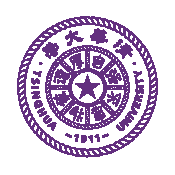
\includegraphics[height=3cm]{thu-fig-logo}}%
  \hspace{4em}%
  \subcaptionbox{第二个小图形,注意这个图略矮些。如果标题很长的话,它会自动换行\label{fig:subfig2}}
      {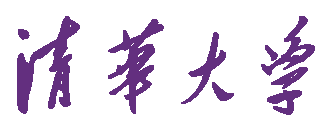
\includegraphics[height=2cm]{thu-text-logo}}
  \caption{包含子图形的大图形(subcaptionbox示例)}
  \label{fig:big1-subcaptionbox}
\end{figure}
\begin{figure}[h]
  \centering%
  \begin{subfigure}{3cm}
    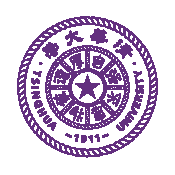
\includegraphics[height=3cm]{thu-fig-logo}
    \caption{第一个小图形}
  \end{subfigure}%
  \hspace{4em}%
  \begin{subfigure}{0.5\textwidth}
    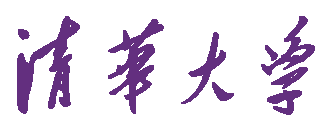
\includegraphics[height=2cm]{thu-text-logo}
    \caption{第二个小图形,注意这个图略矮些。subfigure中同一行的子图在顶端对齐。}
  \end{subfigure}
  \caption{包含子图形的大图形(subfigure示例)}
  \label{fig:big1-subfigure}
\end{figure}

古之学者必有师。师者,所以传道受业解惑也。人非生而知之者,孰能无惑?惑而不从师,
其为惑也,终不解矣。生乎吾前,其闻道也固先乎吾,吾从而师之;生乎吾後,其闻道也亦
先乎吾,吾从而师之。吾师道也,夫庸知其年之先後生於吾乎!是故无贵无贱无长无少,道
之所存,师之所存也。

嗟乎!师道之不传也久矣,欲人之无惑也难矣。古之圣人,其出人也远矣,犹且从师而问焉;
今之众人,其下圣人也亦远矣,而耻学於师。是故圣益圣,愚益愚。圣人之所以为圣,愚
人之所以为愚,其皆出於此乎?爱其子,择师而教之,於其身也,则耻师焉,惑焉。彼童子
之师,授之书而习其句读者,非吾所谓传其道、解其惑者也。句读之不知,惑之不解,或师
焉,或不焉,小学而大遗,吾未见其明也。巫医、乐师、百工之人不耻相师,  士大夫之族
曰“师”曰“弟子”之云者,则群聚而笑之。问之,则曰:彼与彼年相若也,道相似也,位
卑则足羞,官盛则近谀。呜呼!师道之不复,可知矣。巫医、乐师、百工之人。吾子不齿,
今其智乃反不能及,其可怪也欤!圣人无常师。孔子师郯子、苌子、师襄、老聃。郯子之徒,
其贤不及孔子。孔子曰:“三人行,必有我师。”是故弟子不必不如师,师不必贤於弟子。
闻道有先後,术业有专攻,如是而已。

如果要把编号的两个图形并排,那么小页就非常有用了:
\begin{figure}
\begin{minipage}{0.48\textwidth}
  \centering
  
\includegraphics[height=2cm]{thu-whole-logo}
  \caption{并排第一个图}
  \label{fig:parallel1}
\end{minipage}\hfill
\begin{minipage}{0.48\textwidth}
  \centering
  
\includegraphics[height=2cm]{thu-whole-logo}
  \caption{并排第二个图}
  \label{fig:parallel2}
\end{minipage}
\end{figure}

李氏子蟠,年十七,好古文、六艺,经传皆通习之,不拘於时,学於余。余嘉其能行古
道,作师说以贻之。

\hfill —— 韩愈(唐)

\chapter{绪论}
\label{cha:intro}

\section{课题研究背景}
根据中国互联网络信息中心(CNNIC)统计,截至2017年12月,网络直播用户规模达到4.22亿;其中,游戏直播用户规模达到2.24亿,较2016年底增加7756万,占网民总体的29\%,真人秀直播用户规模达到2.2亿,较去年底增加7522万
,占网民总体的28.5\%~\cite{CNNIC}。而据思科公司的数据预测,2016年到2021年的5年间网络直播会增长15倍,到2021年底网络直播会占总视频流量的13\%~\cite{Cisco2017}。目前工业界出现了许多大型的直播平台,比如,国内有斗鱼~\cite{Douyu},熊猫tv~\cite{Panda},国外以Twitch为首的游戏直播平台,具有社交性质的Facebook Live~\cite{Facebook}、Periscope~\cite{Periscope}等,如图~\ref{fig:platform}所示。 而移动网民数量的快速增长,推动直播行业的发展转移到移动端,从2016年下半年开始,移动直播用户赶超PC端用户。大量的统计数据表明,网络直播会成为互联网中越来越重要的存在,而移动直播作为其中占比较大的部分,研究如何优化移动直播的用户体验质量有着重要意义。

\begin{figure}[t]% use float package if you want it here
  \centering
  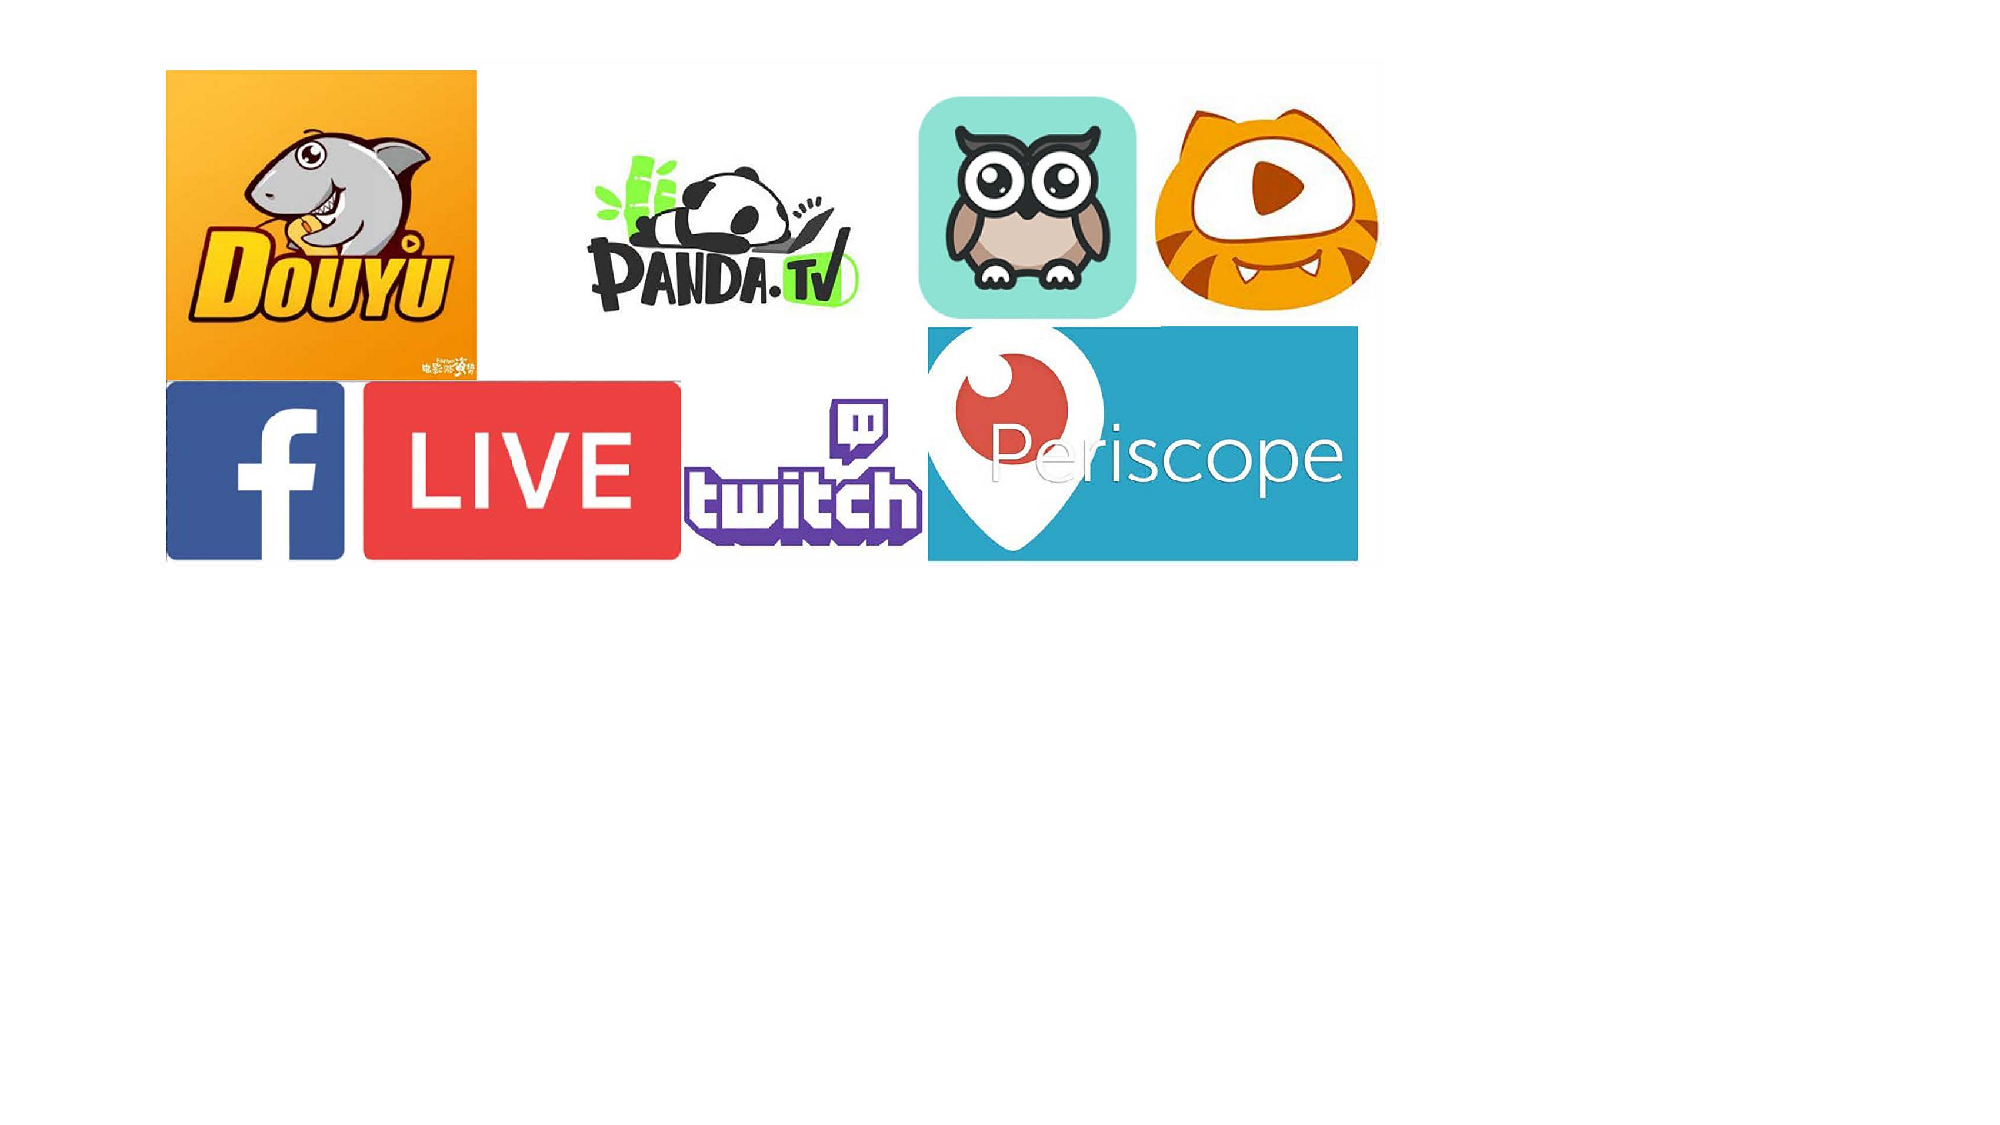
\includegraphics[width=0.7\textwidth]{platform}
  \caption{流行的直播商业平台}
  \label{fig:platform}
\end{figure}

现在火爆的交互直播是由最开始的传统直播演变而来。传统的直播一般只针对“重大事件”,比如ESPN的篮球比赛,奥运会直播等等。传统直播一般预先知道直播的具体时间,运营商会提前为直播源分配好优质充足的链路资源,供直播源上传视频至直播源服务器;源服务器接收到直播视频流后,可能会对接收到的视频流进行一定的转码操作,将RTMP流转码为HTTP流,也可能会将原先单一码率的视频分别编码为多种码率,储存在源服务器上;之后源服务器将编码完的视频,选择合适的码率通过CDN网络,IP组播和P2P~\cite{zhang2005coolstreaming}等分发技术分发到每个CDN边缘节点;观看直播的用户从CDN边缘节点处获取视频。传统直播一般全程使用HTTP协议,为了应对可能出现的网络状况变化,保证用户观看的连续性,传统直播一般会把发送和接收缓存都设置得比较大,导致端到端的时延也较大,为几十秒左右。但随着移动设备的普及,用户已经不再满足于单纯的观看直播,用户开始逐渐成为直播内容的贡献者,传统直播技术此时不再能够满足用户的需求。同时由于LTE等通信技术的发展,低延迟的个人交互直播应运而生,繁荣发展。

RTMP(Real Time Message Protocol),即实时消息传送协议,用于传递音频信息以及视频信息。RTMP协议因其较低的端到端时延在交互直播中得到了广泛应用。RTMP是一种面向连接的实时流式传输协议,在传输开始前RTMP层首先要握手先建立连接,面向连接的传输协议保证了传输的安全性。消息是RTMP传输协议的基本数据单元,消息包含音频信息和视频信息,一般将一个视频帧封装成一个视频消息。而HTTP协议的基本传输数据单元是一个视频块,视频块时长一般为4-10s,只有当完整接收到一个视频块之后,用户端才能正常播放。以视频帧作为RTMP协议的基本传输单元,RTMP协议对应的端到端延时较小。RTMP协议低延时的特性使得它被应用在许多商业直播平台上面,包括Facebook Live, Periscope,熊猫TV,斗鱼等国内外大型直播平台。

尽管学术界目前有很多研究都关注于提升直播平台的用户体验质量,但很少有人研究在直播应用中,如何通过优化主播端的上传质量,从而去优化用户的观看质量。实际上,对于直播应用来说,主播端的视频传输质量非常重要。如图~\ref{fig:architecture}所示,主播端在直播架构中占据着源头的地位,所以主播端的任何延迟或者上传失败都会随着分发网络传递到用户端,影响着全部用户的观看体验质量。除此之外,主播端为用户观看到的视频传输质量设置了一个最高的限制,下游用户的质量不可能超过主播端的质量。因此,主播端需要在可能的情况下上传尽量高清的视频。

\section{主要研究目标和贡献}
个人直播应用虽然由传统直播演变而来,但也不同于传统的直播应用。传统的直播应用的源服务器处上传带宽相对充足稳定,端到端的传输时延一般会在几十秒的量级。但在个人交互直播中,大多数的主播端可能会使用无线网络进行直播,同时由于移动直播中主播端不固定的特性,网络抖动会比较剧烈,网络带宽不稳定。另外,交互直播要求端到端的时延必须在几秒以下,才能满足主播和观众互动的要求。比如,有观众给主播提问或者送礼物,主播需要及时的回应,否则可能会打击观众的积极性。交互直播的这些特性为主播端传输优化带来了新的挑战,可以总结为一句话:在抖动的带宽环境下尽量提供较高的传输质量和用户体验,包括视频质量和端到端的延时等要求。

对于个人交互直播来说,无线网络环境可能会带来新的质量问题。为了验证是否现有的直播平台能否有效的应对无线网络环境,我们首先进行了一定的测量实验。我们选择了两个流行的直播应用,斗鱼和Twitch,通过在主播端控制带宽变化,监控主播的出口吞吐量,发现这些直播平台都普遍存在着两个质量问题:
\begin{enumerate}[1)]
  \item 短暂的网络带宽抖动在应用层会产生放大效应,从而导致长时间的视频质量下降。测量过程中,我们发现如果主播端发生了1s的网络抖动,那么应用层观测到的结果是主播端会有数秒的上传暂停的情况出现。因为交互直播要求端到端的时延尽量小,所以系统各个部分的缓存都很小,暂停数秒上传反映到观众端,则是几秒的黑屏或者暂停。
  \item 现有的直播平台都无法有效应对带宽长时间降低的状况。由于设备移动的原因,可能导致小区间切换,WiFi和蜂窝网切换等问题,主播端经常会出现长时间的带宽波动。但经过我们的测量发现,目前的商业实现都不能有效的解决这个问题。目前的商业平台在带宽降低的状况下,依然维持着初始的码率,视频产生速率远远高于网络容量,从而引起严重的视频质量下降。
\end{enumerate}

通过对开源直播应用源码的分析发现,应用层的放大效应是由于RTMP协议的丢包行为导致。当视频帧的队列溢出时,主播端会主动丢包,丢包导致剩下的一些视频帧无法解码,从而用户端会观测到长时间的视频卡顿。而且,一些简单直接的方案,例如,增大视频帧队列的长度,或者换用其他的丢包方式,都会带来一定的质量损失,或者增大端到端的时延,或者降低视频的质量。比如,增大主播端的视频队列长度,可以很好的解决短暂的带宽下降,但端到端的最高时延也会相应的增大。

另外,对于长时间的网络带宽降低,一个可能的解决方案是码率自适应带宽。但现有的方法都集中在研究点播场景下的自适应码率,这些在点播领域效果比较好的自适应码率方案,在主播端表现不好,因为点播情况下视频的队列长度一般维持在10s左右。而主播端的视频队列通常只有1s左右。由于更小的视频队列长度,主播端准确的码率自适应更加具有挑战性。

本文中,我们提出了一整套的解决方案,简称为GVBR(Greedy Variable Bitrate Solution),大大提高了交互直播中主播端的视频质量。我们的主要出发点是主播端的质量问题可以通过跨层协同设计来解决。GVBR主要包括三层,RTMP层,GoP级别,以及帧级别,三个级别的优化目标都是保证视频的质量和及时性。 RTMP层的配置调整主要是去选择最优的关键帧间隔,因为过小的关键帧间隔会导致视频压缩比过高,视频质量损失,而过大的关键帧间隔会导致放大效应带来的丢帧过多;GOP层面根据预测的带宽和视频帧队列数据量去自适应选择每个GOP的码率;帧级别的解决方案主要是一个智能丢帧策略,尽可能多的减少放大效应。虽然我们的整套解决方案修改了视频流协议的两层,但所有的改动都不用修改内部逻辑,或者是更改可调的参数(例如,关键帧间隔),或者是改变软件中的控制逻辑(丢帧的逻辑和码率自适应策略)。

通过仿真,我们说明好的RTMP层协议可以大大的提高视频质量。通过改变关键帧间隔,我们测量不同关键帧间隔对应的视频质量和丢帧数,给出关键帧的最优选择范围;智能丢帧策略与离线最优算法和默认丢帧策略做对比,相比于默认策略减少了15\%的丢帧,和最优策略有5\%的差距。本文选择了动态码率在点播领域最新的两个算法作为对比算法,与我们提出的算法GVBR作对比。通过在不同网络环境下的大规模仿真,我们发现GVBR同目前现先进的算法比,可以减少至少50\%的丢帧;而相比原始默认的算法,在保证同样视频码率的情况下,视频卡顿的概率减少90\%。

总而言之,本文有两个主要的贡献点:
\begin{enumerate}[1)]
  \item 我们是第一个把目光着眼于提升主播端视频质量的。通过对于流行视频直播平台的测量,我们发现主播端普遍存在两个质量问题,网络层短暂的带宽波动会在应用层导致长时间的视频卡顿,并且现在的直播应用都无法有效解决长时间的带宽波动。
  \item 我们提出了一整套解决方案,去协同解决观测到的视频质量问题,包括帧编码参数和智能丢帧策略,以及GOP级别的比特率自适应策略。
\end{enumerate}

\section{文章组织架构}
本文的内容共有六章,按照如下方式展开:

第一章是绪论部分,主要介绍交互直播的发展过程,简要概率了我们的研究目标。

第二章介绍了直播相关的一些背景知识,主要包括个人直播的架构、特点、以及性能要求。

第三章从我们搭建的平台出发,给出测量中发现的问题,目前的直播平台并不能很好的满足性能要求;并给出在商业平台中的测量,实验发现商业平台也不能很好的解决上述问题。

第四章,剖析直播软件的源码,发现上述问题出现的原因,主要是由于视频编码输出的码率不能实时的按照带宽变化,最后我们给出了一些优化设计的原则。

第五章根据设计准则,我们设计了一整套的解决方案,涵盖帧级到GoP级。

第六章与之前的算法进行比较,进行充分的实验仿真。

第七章总结现有的工作,并展望未来的研究方向。


\chapter{研究现状概述}
随着移动通信技术和个人设备的迅速发展,移动直播的应用呈现井喷式发展。据思科公司的数据预测,未来3年网络直播会占据总视频流量的13\%。移动直播用户数量大幅度增长的同时,用户对于直播服务质量的要求也随之提高。

传统直播能够将视频通过网络分发给大量的用户,为广大用户提供视频服务。但传统直播的不足之处在于要求为主播端预留专线带宽,且端到端的时延较大。在大量用户渴望成为直播内容贡献者的今天,要求每个主播都拥有专线带宽并不可行;而且传统直播的高时延无法满足观众对于直播互动性的要求。


\section{直播传输优化研究现状}
\subsection{直播发展现状}
传统直播的系统架构和交互直播基本相同,传统直播也由三部分组成,视频源端到源服务器,源服务器到CDN边缘服务器,CDN边缘服务器到观众。但传统直播的视频源端到源服务器的链路一般为预先分配的专有链路,所以传统直播研究的重点集中在源服务器到观众端的部分。从源服务器到观众端主要有两种分发架构,CDN网络~\cite{mukerjee2015practical}和P2P网络~\cite{liao2006anysee}~\cite{hei2007inferring}~\cite{magharei2007mesh}。CDN网络分发和P2P网络分发各有优缺点,CDN网络分发时会根据网络负载去选择负载轻的服务器,根据用户的带宽去选择合适的码率。当网络中服务器负载不高时,CDN网络分发能给终端用户提供较高的体验质量。但为了保证用户的体验质量,CDN网络需要保证网络各服务节点负载不高,因此需要配置相当数量的服务器,运营成本较高。相比较而言,P2P网络具有高度可扩展性,对服务器的负载要求较少,然而P2P这种去中心化的合作方式大规模应用的话会有一些缺点,比如,用户接收到的视频质量低,节点之间负载不均衡,无法进行网络监管等问题。

\begin{figure}[h]% use float package if you want it here
  \centering
  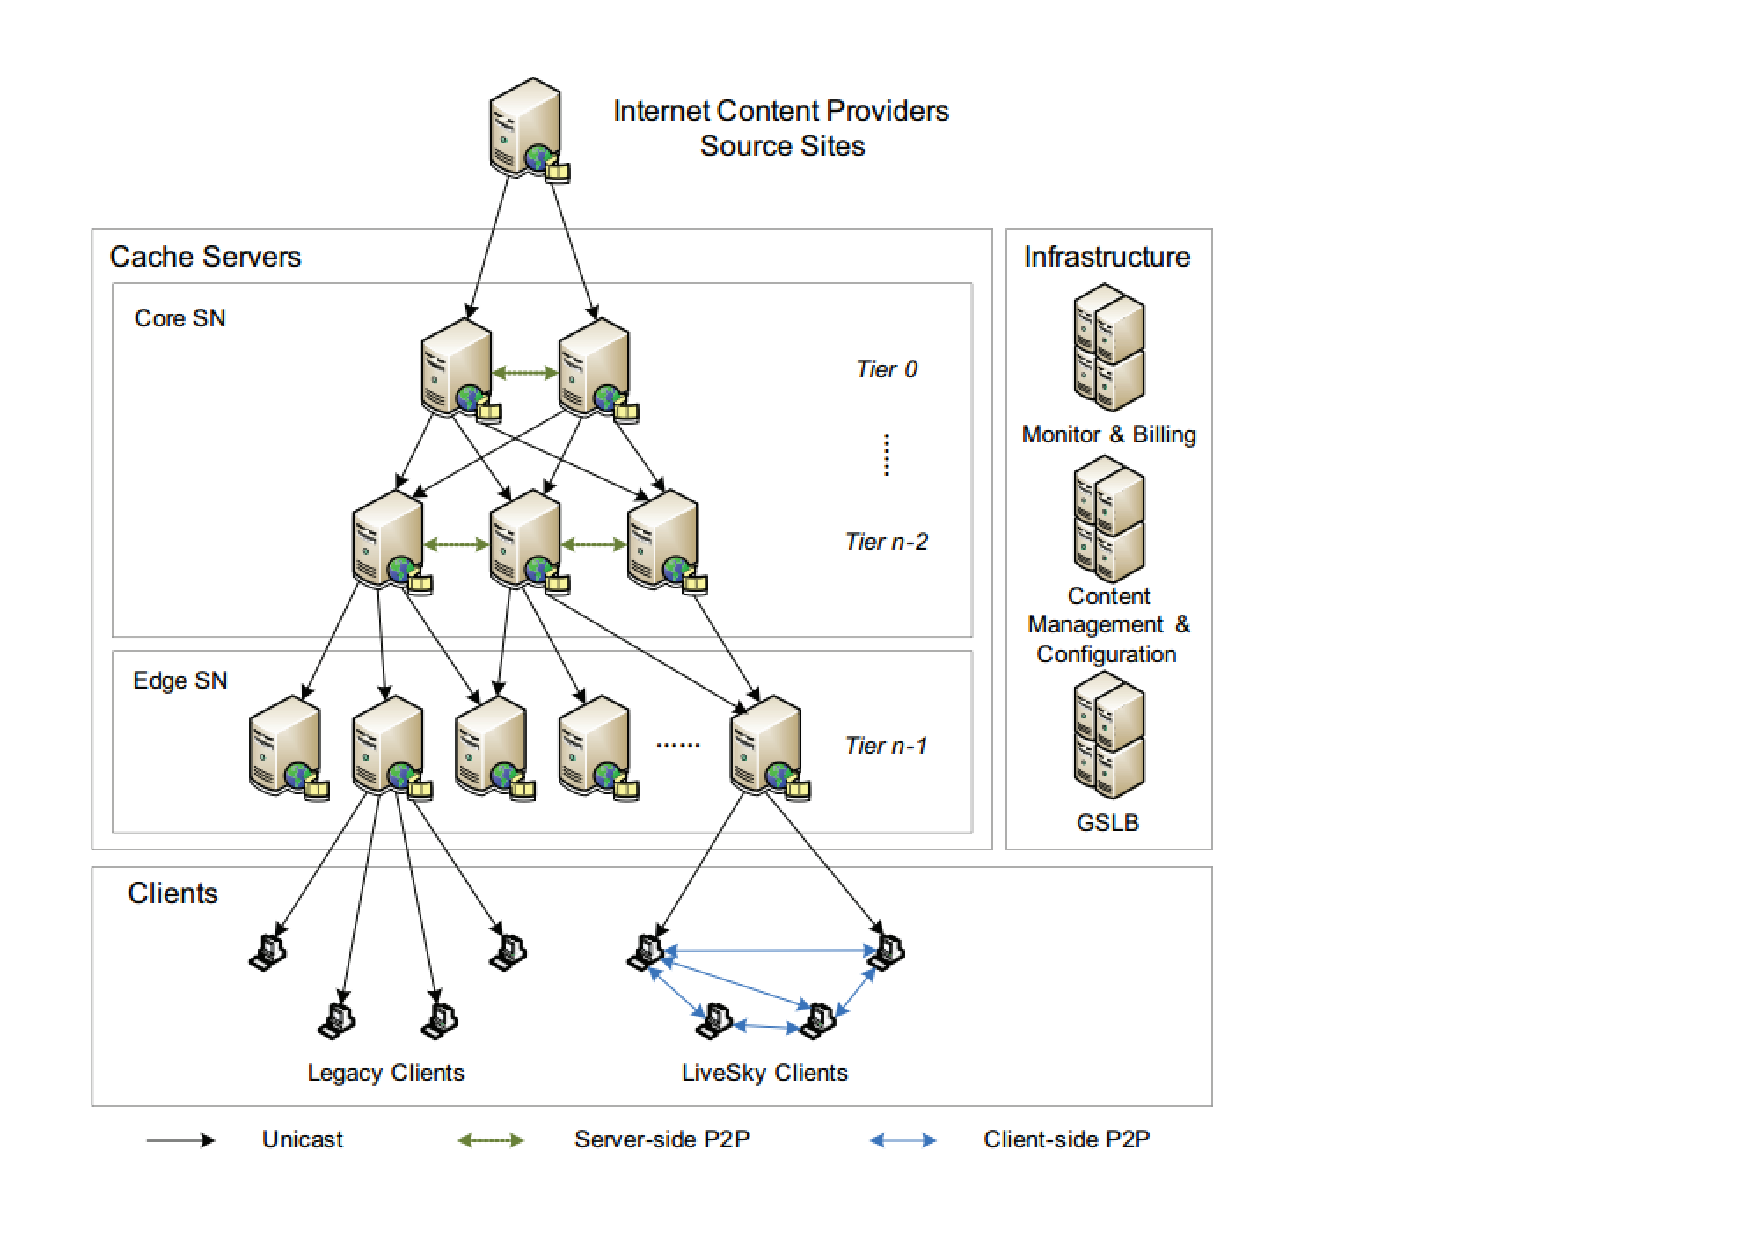
\includegraphics[width=0.9\textwidth]{livesky}
  \caption{LiveSky系统架构图~\cite{yin2009design}}
  \label{fig:livesky}
\end{figure}

Yin等学者~\cite{yin2009design}提出了P2P网络和CDN网络混合分发的LiveSky架构,并在实际中部署,LiveSky的系统图如图~\ref{fig:livesky}所示。针对P2P和CDN的联合架构,Yin等人设计了一个分段阈值式的资源动态分配机制,在用户规模增大的情况下依然能提供良好的视频观看体验。同时他们利用CDN的边缘服务器和重定向机制去解决P2P系统的不足,使得采用NAT地址转换的用户也可以完成上传,保证对现有网络而言的公平性。

学术界目前关于个人交互直播的研究多数还只是着眼于分析直播用户的行为,以及对交互直播系统框架的解剖。Zhang等学者~\cite{zhang2015crowdsourced}通过爬取Twitch网站~\cite{Twitch}提供的数据,抓取本地主播端的流量勾勒出了交互直播的内部架构;另外,通过对Twitch网站数据两个月的抓取,Zhang等发现用户的观看行为基本由重大事件和主播决定。另外,观众端感受到的时延会严重影响观看的交互体验。Twitch将直播视频分发和信息发送分开来实现,因此直播消息的时延很短,视频时延很长,两者之间差别很大。另外,Zhang等学者改变主播端的带宽容量发现,主播端的带宽容量会明显影响直播视频播放的流畅性。

Meerkat和Periscope是另外两个国外主流的移动直播应用,主要部署在移动端。Matti等作者重点研究了Periscope应用的用户体验质量~\cite{siekkinen2016first},主要是播放流畅性,延迟和能量消耗等相关因素。Periscope的接口信息是通过HTTPS加密的方式传播的,Matti等人通过建立透明代理的方式去截取Periscope应用接口的信息。并且Periscope的接口并不直接给出平台的总用户数信息,只提供邻近地区的用户数,Matti等人通过深度挖掘每个地区用户量的方法去组合获取实时的总用户量。另外,Periscope主播用户的粉丝数呈现长尾分布,主播用户的粉丝数会影响主播用户的积极性,粉丝数少的主播直播时长会相应的变短。

直播应用一般会给每个主播分配一个独一无二的ID,Wang等作者利用这个特性~\cite{wang2016anatomy},以高频率的轮询算法随机观看直播,去计算Meerkat~\cite{Meerkat}和Periscope的用户数和主播数。另外,Wang等人发现Periscope直播平台为了增加系统的可拓展性,在用户数小于100时,直接使用RTMP协议进行分发,当用户数超过100时,多出来的用户通过HTTP协议进行直播视频分发。Wang等人对两种协议情况下主播端到用户端的每一段引入的时延进行了分析,发现使用HTTP协议分发视频,相比于使用RTMP协议直接获取视频,引入了切块时延和用户请求延时。 另外,使用HTTP协议进行视频分发时,用户端的缓存策略一般比较保守,缓存时间较长,从而导致较大的缓存时延。

关于优化直播传输质量的研究很少,但通过优化主播端的传输质量来优化用户体验质量的研究更加稀少。

\subsection{直播协议研究现状}
在众多视频传输协议中,HTTP协议凭借广泛部署的CDN网络以及易穿透防火墙,服务器代码开源等特性,逐渐成为视频点播领域的主流协议~\cite{li2013two}。现在的HTTP协议在视频方面主要有APPLE的HLS(HTTP Live Streaming)协议~\cite{Apple}和DASH(Dynamic Adaptive Streaming over HTTP)协议~\cite{stockhammer2011dynamic}~\cite{sodagar2011mpeg},两者的原理基本相同。HTTP协议都会对视频进行切块操作,将一个完整视频切为许多4-10s的视频块,视频块是传输和处理的基本单元。HTTP协议的延时较高,主要是因为只有当一个视频块完整的产生后,CDN端才开始分发,用户端才能开始播放,所以不可避免的至少有一个视频块的延时,称为切片时延。由于切片时延的存在,且切片时延一般为数秒的量级,HTTP协议的延时一般都较大,因此HTTP协议在直播领域的应用较少。

针对HTTP协议的切块时延,一个比较直接的解决方案是减少视频块的时长,减到直播情景可以接受的时间长度,减小由于视频切块带来的时延。但是若直接减少视频块的时长,会导致HTTP请求数的倍速增长,使得HTTP服务器的负载过大。客户端发起的HTTP请求数和视频块的时长成反比,比如,对于一个60秒的直播视频,如果每个视频块是4秒,总的请求响应数目为15;但当我们把视频块的时长缩短为1秒时,总的请求响应数目会增长为60。因为每个HTTP请求和响应都会有头部报文,倍数增长的请求响应给服务器和网络设备带来了额外的处理开销,这对HTTP视频流的可扩展性造成了极大的影响。

\begin{figure}[htb]
  \centering%
  \begin{subfigure}{0.45\textwidth}
    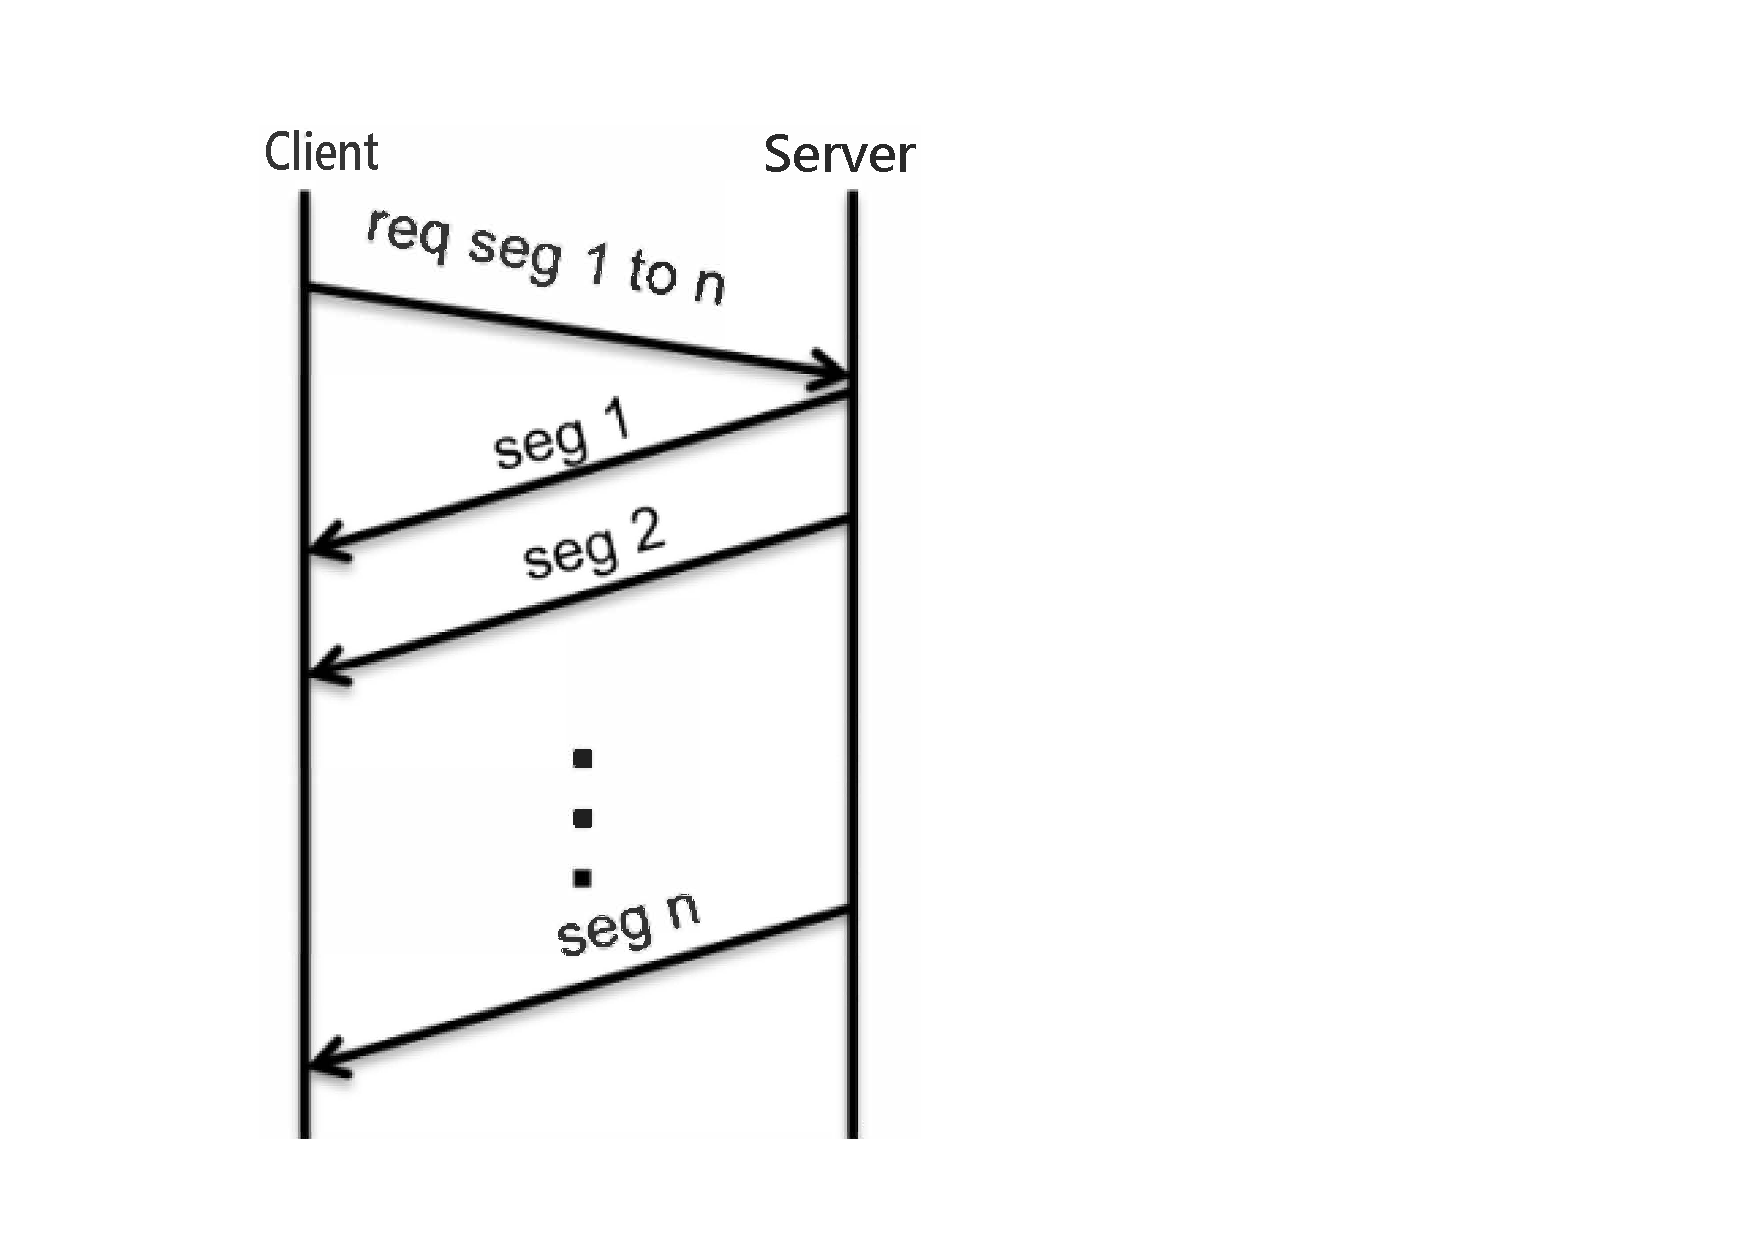
\includegraphics[width=\textwidth]{all-push}
    \caption{一次推送全部内容}
    \label{fig:all_push}
  \end{subfigure}%
  \hfill
  \begin{subfigure}{0.45\textwidth}
    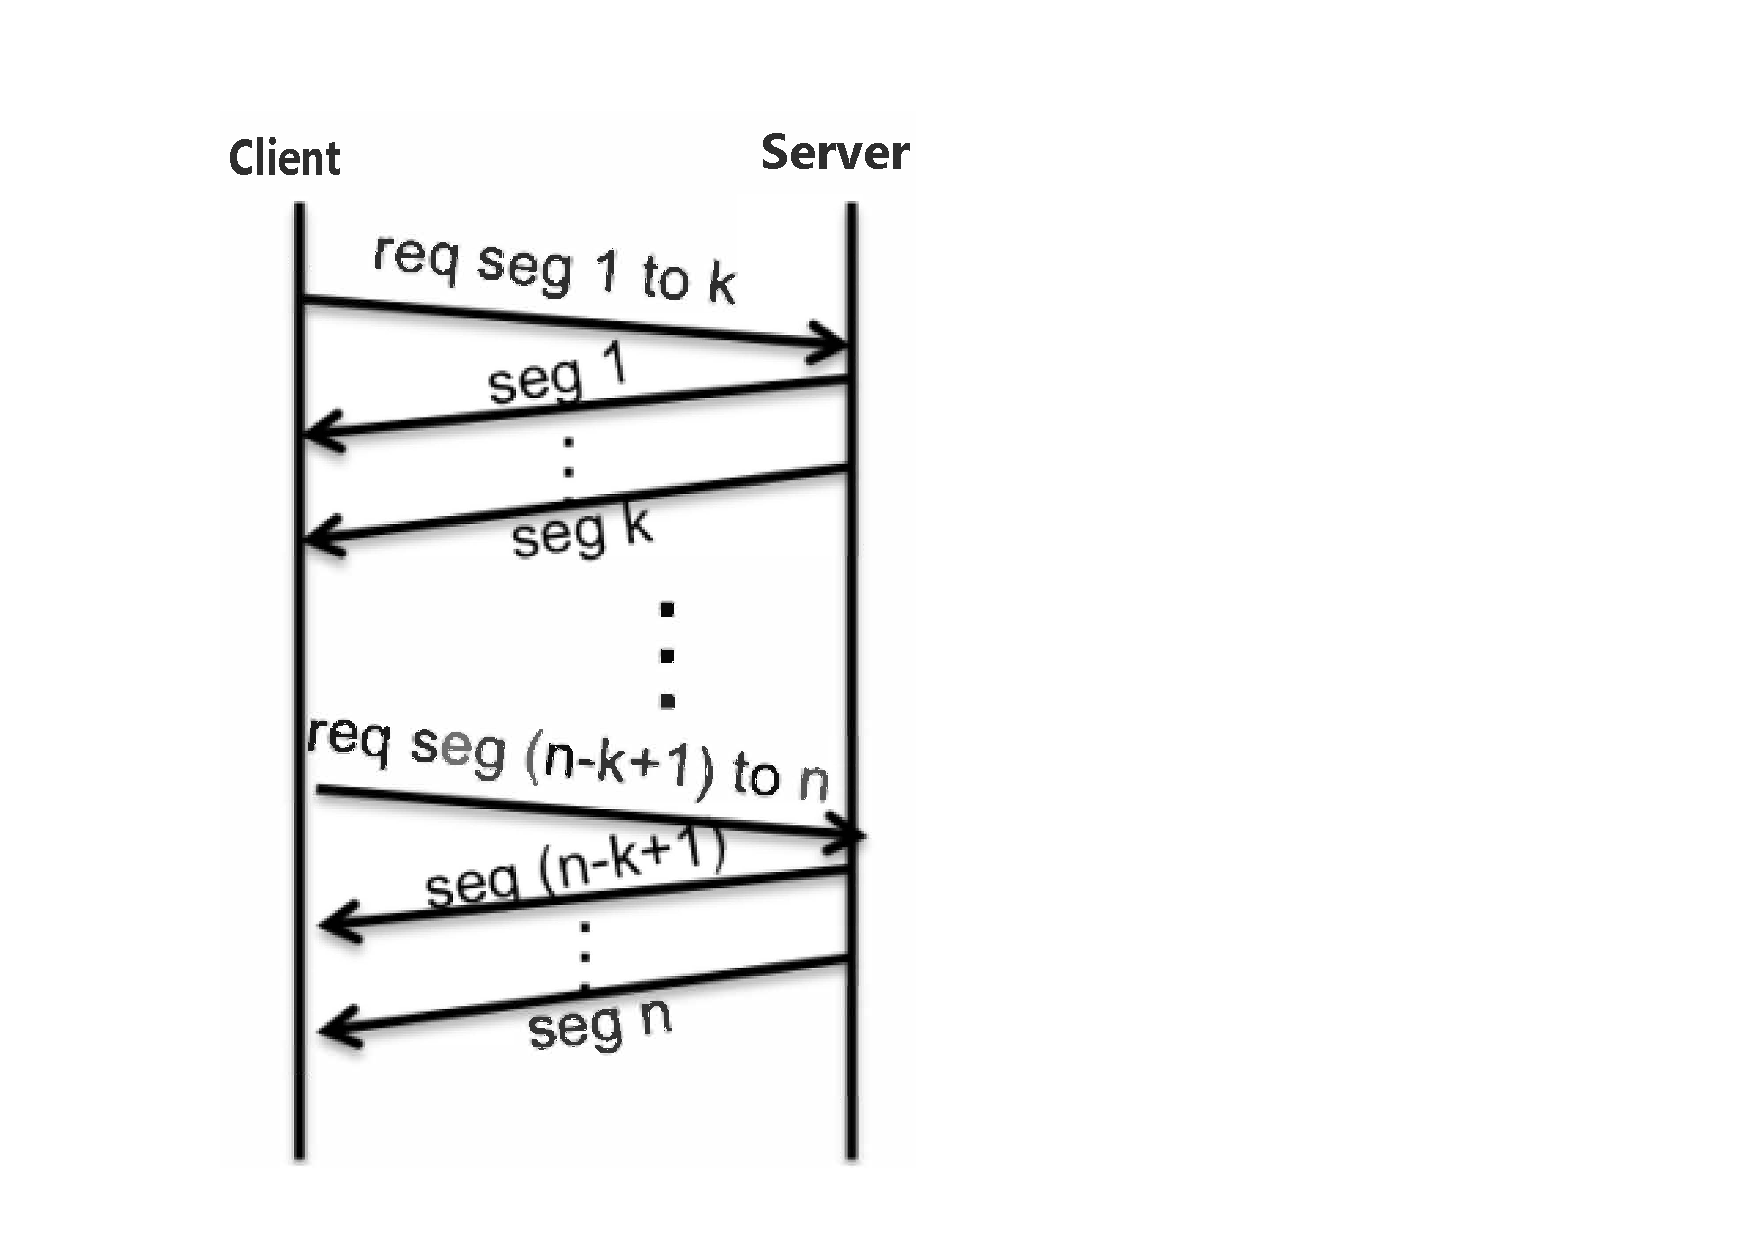
\includegraphics[width=\textwidth]{k-push}
    \caption{一次推送多个内容}
    \label{fig:k_push}
  \end{subfigure}
  \caption{HTTP协议2.0版本的新特性~\cite{wei2014low}}
  \label{fig:push}
\end{figure}

学术界有一些研究尝试将HTTP技术应用到直播中来,研究如何解决HTTP协议的切块延时过长问题。HTTP协议2.0版本引入的服务器推流特性允许服务器直接将资源推流到客户端,不需要客户端去明示的请求资源,这个特性极有可能打破视频块大小和请求数之间的反比关系。Wei等学者便尝试利用HTTP协议2.0的推流特性去减少切块时延~\cite{wei2014low},因为HTTP协议2.0并不是专门的视频传输协议,因此Wei等人提出了一个定制的视频推流策略。利用HTTP服务器推流减少时延的主要思路是尽可能减少视频块的时长直到满足时延要求。推流策略需要解决的问题有两个方面:推哪些内容和什么时候推。文章给出了两种策略,一次请求推送全部内容和一次请求推送多个内容,如图~\ref{fig:push}。文章通过大量的实验说明,使用服务端推流的特性,直播的时延可以大大的降低。

HTTP协议的分块传输编码机制也被用来减少HTTP协议中端到端的时延~\cite{swaminathan2011low}。Swaminathan等学者在文章中提供了两种减少端到端时延的方案,分别是服务器等待策略和分块编码策略。服务器等待的策略和原来的视频块策略相比,只做了些微的修改。最根本的改变是客户端请求正在生成的新视频块,而不是已经生成的视频块。为了达到这一目的,客户端请求描述文件中最新视频块的后面一个视频块。因为请求的视频块尚未生成,所以服务器在收到请求后一直处于等待状态,直到视频块生成为止。服务器等待的策略减少了将近一个视频块的时延,但这个优化的程度还远远不够。为了进一步优化端到端时延,Swaminathan等人进一步提出了分块编码策略。和服务器等待策略相同,分块编码策略也总是请求后面一个视频块。分块编码策略中,服务器端将视频块切分为均匀的多个视频片段,收到客户端的请求后,将编码完成的视频片段先发送出去,之后陆续将剩余的视频片段发送出去。不同于最简单的HTTP协议,HTTP分块编码允许在服务器端维护一个HTTP长连接,客户端只需要一次请求,就可以接收数次响应消息。利用分块编码,同时将每个视频块的时长增大,分块编码达到了减少时延的效果,将时延降低为1~2个视频片段的时长。

Bouzakaria等人利用GDR(Gradual Decoding Refresh)~\cite{hannuksela2003random}技术去编码,将直播视频编码成ISO基本媒体文件格式,并在传输层使用分块编码传输策略去减少HTTP协议的时延~\cite{bouzakaria2014overhead}。GDR技术是相对于用完整的一个视频帧来刷新的技术而言的。传统的完整帧刷新编码技术有一定的缺点,关键帧相对于其余的帧体积过大,容易对网络造成冲击,导致网络抖动。而GDR技术将关键帧分散到几个非关键帧中,缓解了对网络带来的冲击。Bouzakaria等人采用和Swanubathan类似的思路,改造了DASH传输协议的MPD文件,在原有MPD文件中添加了一个字段:有效时间偏差。有效时间偏差代表了新的视频块可以请求的时间,即使新的视频块可能只产生了一部分片段。有效时间偏差字段使得客户端提前得知有新的视频块产生,并提前发起请求,有效减少了HTTP协议的延迟。

上述研究都一定程度上解决了HTTP协议的低时延问题,但目前商业化平台应用仍然只在视频分发时使用HTTP协议,因此我们研究的重点依然集中在主播端使用较多的RTMP协议。

\subsection{码率自适应研究现状}
关于码率自适应研究的文章很多,其中大部分都集中在点播领域~\cite{mao2017neural}~\cite{akhshabi2011experimental}~\cite{petrangeli2016qoe}。点播领域的码率自适应算法可以分为三类:基于带宽的,基于缓存的,以及两者的结合。

FESTIVE~\cite{jiang2014improving}就是典型的基于带宽的码率自适应算法。FESTIVE通过测量现有的商业级播放器,包括Netflix,Adobe OSMF等,发现当多个动态码率播放器共享同一链路时,会出现带宽分配不均匀的问题。另外,高码率和码率的稳定性在动态码率情况下也是应该考虑的重点。针对这三个性能指标,FESTIVE提出了一整套的解决方案。FESTIVE采用随机调度视频块的方式去减缓其他播放器下载视频占用带宽带来的带宽探测误差,从而尽量避免带宽分配的不均匀;用状态转移的方式去选择码率,拟合码率和预估带宽之间的偏差;码率延迟更新策略,以达到高码率和码率稳定性之间的平衡。

大多数码率自适应算法都是基于带宽去选择码率~\cite{li2014probe}~\cite{akhshabi2012happens},但是对于无线网络环境,尤其是在移动设备的情况下,带宽变化剧烈,很难去精确的预测带宽。Huang等人~\cite{huang2015buffer}首次创新性的提出了基于缓存的数据量去选择码率的算法。视频播放一般可以划分为两个阶段:启动阶段和稳定阶段。视频开始播放时,缓存的数据先从零开始积累到一个阈值,之后边下边播,缓存进入稳定阶段。基于缓存选择码率的算法基于一个想法:当缓存数据量较大时,用户端可以选择较高点的码率,提高码率的收益;如果缓存数据量较小,那用户端应该保守一些,选择较低点的码率,以保证不卡顿流畅播放。在开始阶段,缓存相关信息量较少,此时利用带宽预测的信息选择码率是很有必要的;但一旦进入稳定阶段,缓存数据量相关的信息充足时,只根据缓存去选择码率也可以性能很好。

Yin等学者~\cite{yin2015control}利用模型预测控制理论(MPC)来优化码率选择。MPC尝试预测未来一段时间的网络环境,模拟未来一段时间的系统状态,遍历求得一段时间的最优解决方案,然后只采用下一时隙的解决方案,循环往复。MPC将之前基于码率和基于缓存的方案结合起来,在优化时将码率和缓存同时纳入了优化空间,MPC的优化空间如图所示。另外,求一段时间内的最优方案有更大可能会优于某一时刻的最优。码率遍历选择的算法由于其高时间复杂度在实际运行中会面临问题,Yin等人提出了基于查询缓存结果的FastMPC算法,相对现有的所有算法提高了10\%-15\%的平均用户体验质量。

点播和直播领域的码率自适应主要有两点不同。第一个不同点是时间粒度,点播动态码率的粒度为一个视频块,而一个视频块持续4-10s秒时间;直播码率变化的粒度为一个GoP或者更小,一个GoP通常为2秒左右。第二个不同点是缓存队列的大小,点播时通常会缓存数十秒以防止播放的卡顿;而直播时缓存最少不超过1秒,否则会增加端到端的时延。

学术界也有一些关于直播如何使用码率自适应技术的研究。Pires等人~\cite{pires2014dash}通过对Twitch平台用户规模以及用户行为的研究,提出可以应用码率自适应技术分发直播流。直播的流程如图~\ref{fig:architecture}所示,如果想要应用码率自适应技术进行视频分发,需要在源服务器处进行转码,将主播端上传的单一码率视频转码为多个码率,之后用户选择自己适合的码率。Twitch平台上并发的主播数量很多,对所有主播直播的视频进行转码会需要消耗大量的计算资源。文章考虑主播的观众数,转码带来总的用户体验质量的提升以及资源消耗等因素的折中,选择部分主播进行转码操作。

Bouzakaria等学者~\cite{bouzakaria2014overhead}尝试用动态码率自适应技术去实现超低时延的直播。动态码率自适应技术的时延主要有几个部分构成:切块时延,下载视频块的时间,以及用户端的缓存时长。如果将视频块切成更小的数据块在网络中传输,切块时延也会减小为小视频块的时长。之前的CDN和播放器都是在接收到一个完整的视频块之后,才开始转发以及播放。为了进一步减少时延,Bouzakaria等学者修改了视频信息描述文件,并且使用HTTP协议的分块传输编码,一旦接收到一个视频块的一段,就可以开始分发和播放,将原有的一个视频块的时延减少为一段的时延。

\begin{figure}[h]% use float package if you want it here
  \centering
  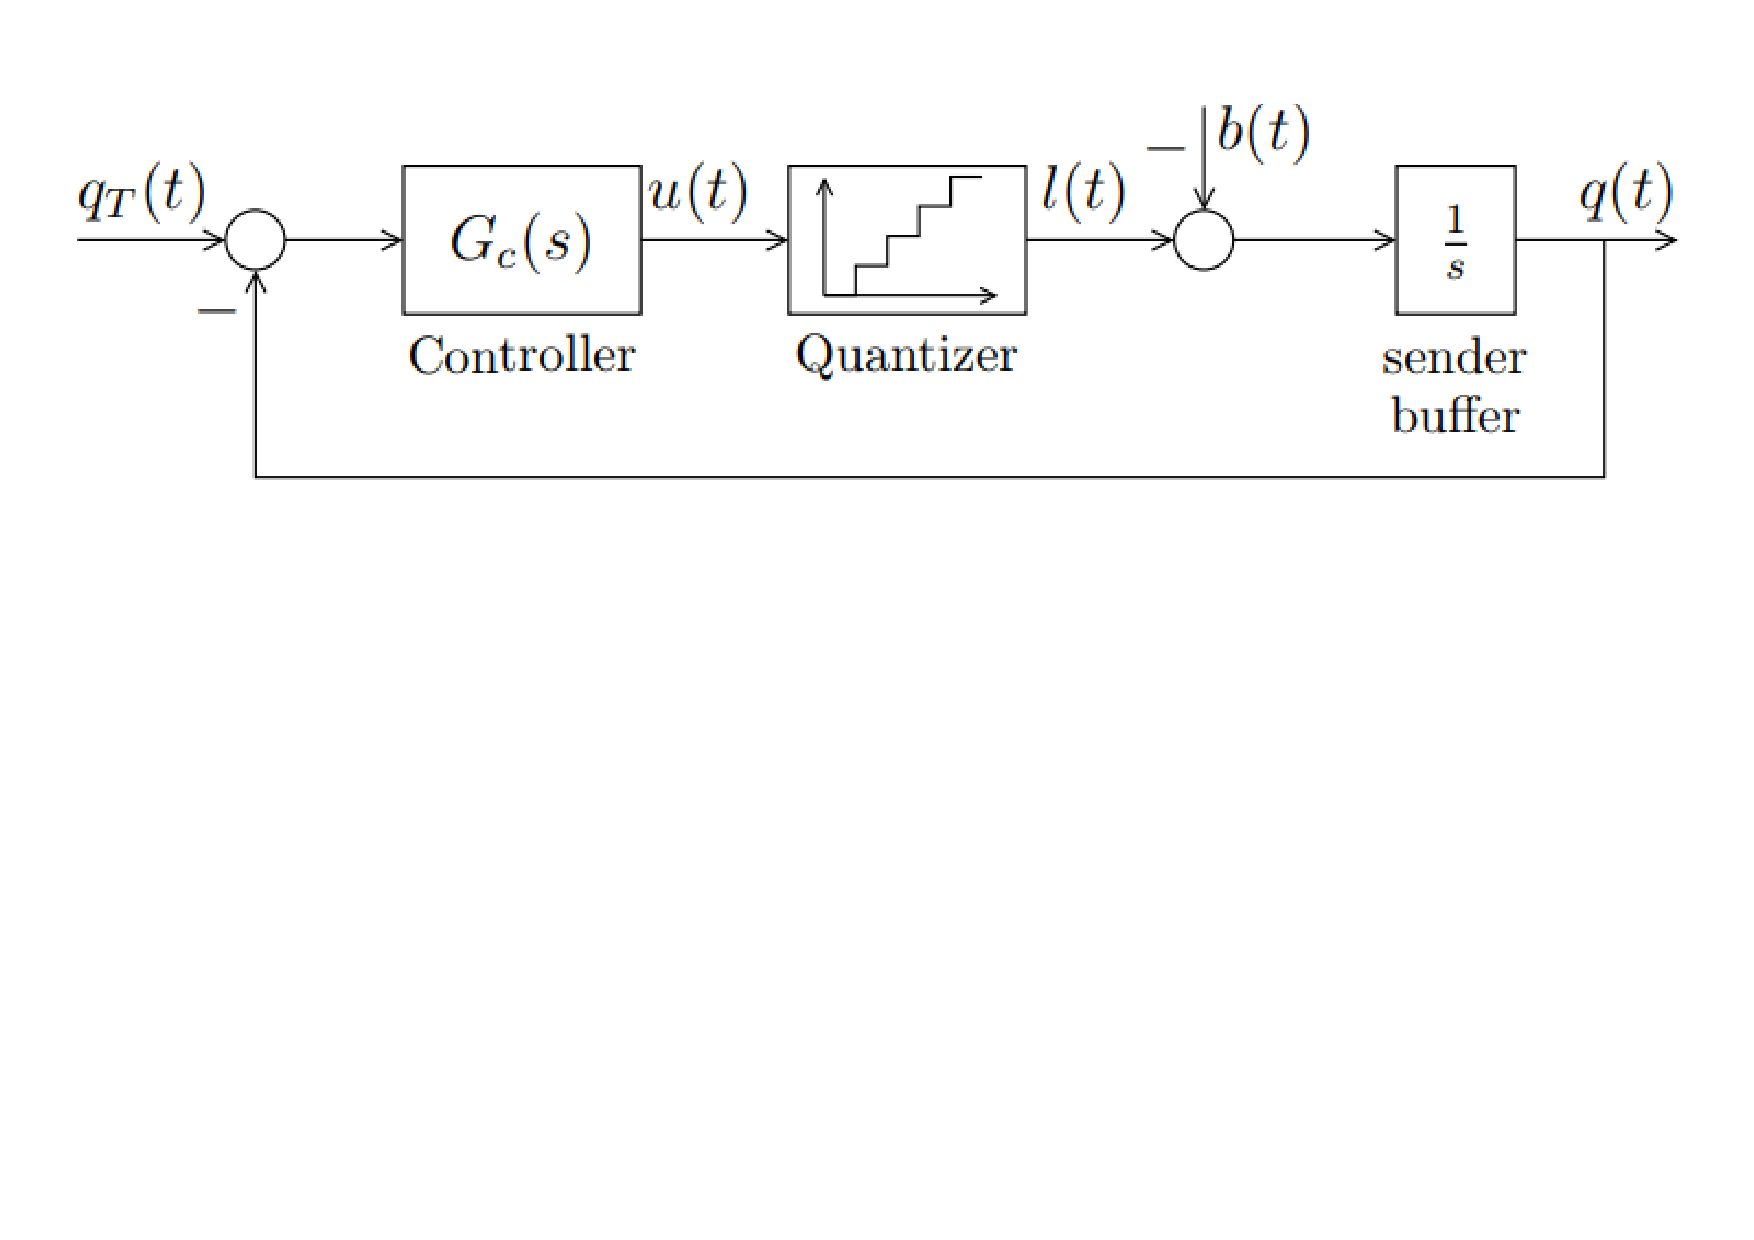
\includegraphics[width=0.9\textwidth]{feedback_control}
  \caption{反馈控制理论~\cite{de2011feedback}}
  \label{fig:feedback_control}
\end{figure}

De等人~\cite{de2011feedback}用反馈控制理论去选择最优码率。不同于之前的启发式算法,反馈控制理论可以得到一个可预测的系统状况,更方便下一时隙的码率选择。控制器工作流程如下图~\ref{fig:feedback_control}:发送端的缓存大小作为输入,$q_T$是发送端缓存的阈值。控制器的激活部分,以发送端现在的缓存大小和阈值$q_T$的差作为输入,输出控制信号。输出的控制信号经过量化,选择最大的小于量化后的值的码率,即为最后所选择的码率。

上述关于在直播中使用码率自适应技术的研究多数关注于如何大规模部署码率自适应技术,以及超低时延的码率自适应技术,De等人的研究虽然关注于如何选择码率最优,但是研究的是点对点的直播,且端到端的延时较大。总体来说关于如何优化直播应用主播端的传输质量的研究很少,所以我们的研究也具有一定的挑战性。

\subsection{交互直播的性能要求}
点播情景下对于系统的性能要求一般是三点:高码率,敏捷平滑的码率切换以及低卡顿率。但主播端不同于点播客户端的根本一点在于,点播的客户端是被动接收请求的视频,而主播端负责将摄像头编码产生的视频推送出去。网络状况不好时,点播的客户端接收视频会受影响,导致视频播放出现卡顿;但对于主播端来说,网络状况不好,视频的上传会受到影响,从而导致视频帧从产生到到达用户端的时延过长,用户观看直播的过程中出现黑屏。经过上述分析,移动网络带宽不稳定的状况下,观众和主播间的高交互性要求对直播的主播端提出了如下的性能要求。
\begin{itemize}
  \item 尽可能高的视频质量。视频质量的优劣,和视频的码率,每秒的帧率,以及分辨率都息息相关。在帧率和分辨率固定的情况下,主播端应上传尽可能高的码率到源服务器。源头的码率高,下游的用户才有可能接收到清晰的视频,得到满意的用户体验质量。
  \item 敏捷平滑的码率自适应。交互直播一般都处于移动网络环境下,网络带宽十分不稳定。主播端的码率变化必须足够灵活敏捷,能够快速响应无线网络中的带宽波动。同时,如果应用码率自适应技术,码率的平滑切换也是一个重要的指标。码率的平滑切换要求码率的切换幅度尽量小,切换次数尽量少。
  \item 直播的及时性。为了保证直播的高交互性和用户的高参与度,必须最小化主播端和用户之间的时延,或者限制住最大的时延。端到端的时延要求反映在主播端,则对应于帧发送的时间和帧产生的时间差要满足一定的约束。
\end{itemize}

RTMP协议将视频帧作为基本的传输单位,码率的转换和调整都足够灵活,因此有可能能够满足上述三个性能要求。比如,它在主播端提供了大量可供调节的参数接口,可以调整视频质量,包括每秒的帧率,视频队列的大小,还有丢帧策略的相关参数。理论上来说,合适的丢帧策略需要在视频质量和及时性两者之间维持一个动态均衡~\cite{krasic2003quality}~\cite{singh2004dynamic}~\cite{huang2003adaptive}~\cite{fouladi2018salsify}。直播情境下RTMP协议依然是主旋律。然而,在下章我们会给出,现在开源的RTMP实现以及商业级应用都存在严重的质量问题。

\section{本章小结}
本章首先以传统直播和交互直播的两大关键不同点作为切入点,个人直播相对于传统直播而言个人直播对传输技术提出了更高的挑战,因为个人直播的网络环境一般为无线网络,且用户和主播的强交互性对端到端的时延的要求较高。之后我们给出了现在的较为主流的直播传输框架,在主播端上传时使用RTMP协议,分发时使用HTTP协议借助CDN网络完成。

本章从三个角度来介绍直播传输协议的演变过程,直播框架,直播协议和自适应码率技术。传统直播一般使用P2P网络或者CDN网络来进行分发,还有用两种网络混合的架构来进行分发,交互直播架构的研究目前还只是停留在通过测量去发现现有直播的架构的地步。直播协议方面,RTMP协议因其较低的端到端时延而在直播应用中使用较多。HTTP协议因为至少一个视频块时长的时延而较少应用在直播中,但目前也有一些研究集中在减少HTTP协议的时延方面。码率自适应技术目前较多的研究集中在点播领域,直播方面目前的研究只涵盖了点对点的直播,多用户情景的研究较少。

另外,本章给出了交互直播的三点性能要求,高码率,少切换以及端到端的时延。后续的几章内容主要通过测量发现直播系统中的问题,并尝试设计出一套相应的解决方案。

\chapter{主播端的视频质量问题}
我们用开源的直播应用和服务器搭建了一个实验平台,测量在无线网络环境下,直播应用能否有效的应对复杂的网络状况。通过测量,我们发现开源主播端的实现在运行过程中会遇到传输质量不好的问题,尤其是当网络带宽发生抖动时。为了验证目前直播平台的商业实现是否也存在类似的问题,本章我们测量了一些流行的个人直播应用,如斗鱼和Twitch。大量的测量表明商业级的实现也存在一样的问题。之后我们通过跟踪开源直播应用的源码实现,找出了问题发生的原因。

\section{直播系统架构}
为了解决传统直播面临的这些问题,交互直播应运而生。个人交互直播与传统直播相比,有两大关键不同点:
\begin{itemize}
\item 个人移动设备作为主播端。传统的直播,比如ESPN,都是使用预留的专线连接将摄像机捕捉的高清原始视频传输到特定的源内容服务器,内容服务器将原始的视频转码切分为视频块,分发给每个观看的用户。个人交互直播的不同点在于,用户借助移动设备通过无线网络上传直播视频到源服务器,源服务器分发的过程和传统直播相同。无线网络环境下,移动主播经常会面临和别人一起竞争带宽的情况,同时由于主播的移动和移动环境中复杂的无线信号,个人交互直播可能遭受更多变的网络环境,面临的传输挑战更加严峻。
\item 移动直播要求主播和用户间的交互性。在传统的体育直播中,用户只是被动的观看直播,没有交互行为,也不需要得到反馈。交互直播由于存在主播和用户间的互动行为,端到端的时延至关重要,端到端的时延决定了主播和用户的交互体验。例如,如果用户给主播送礼物或者点赞,主播应尽快回复表示感谢,如果端到端的时延依然是传统直播的几十秒,用户的体验效果将会非常差。高交互性使得直播的延迟最多为几秒,远远小于传统直播的几十秒左右的端到端时延。
\end{itemize}
移动网络环境和高交互性的要求为优化交互直播的传输质量提出了很大的挑战。

\begin{figure}[h]% use float package if you want it here
  \centering
  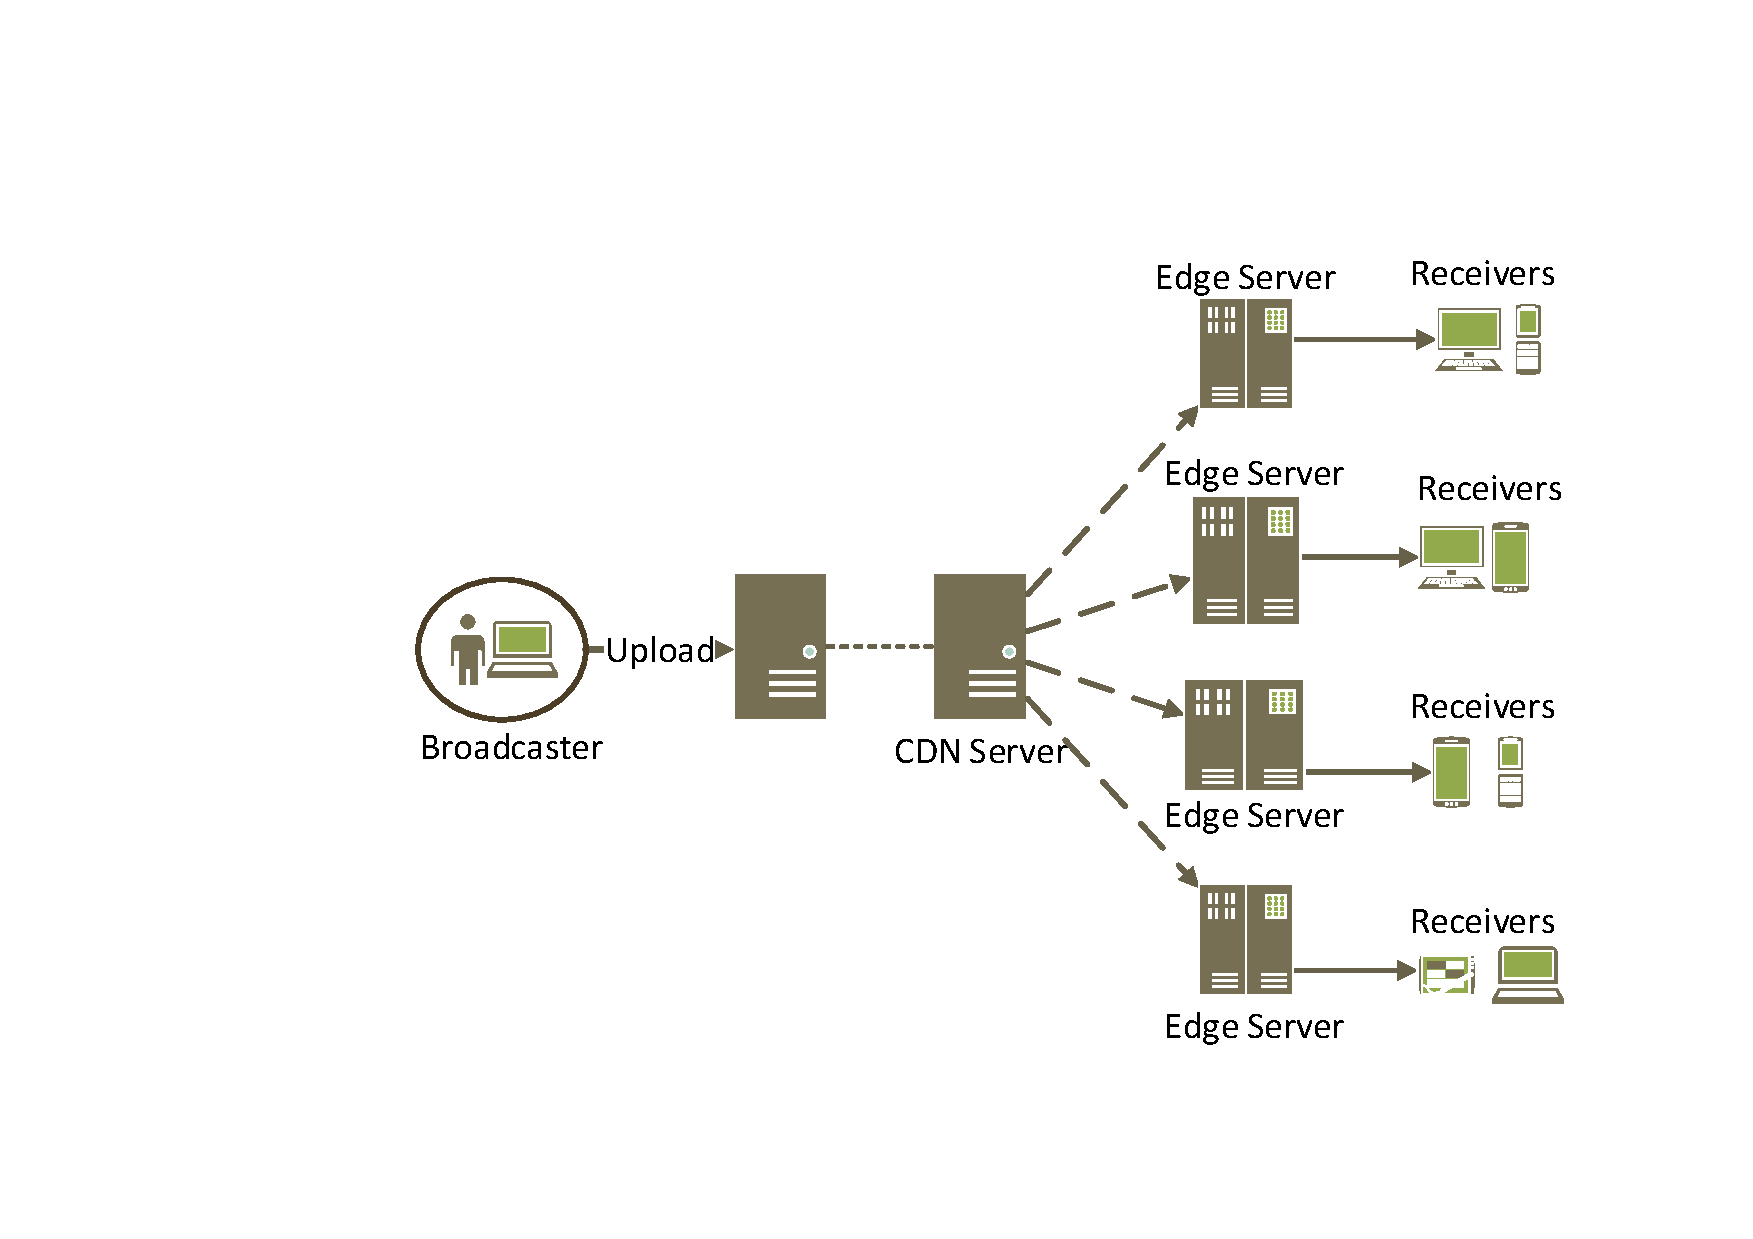
\includegraphics[width=0.8\textwidth]{architecture}
  \caption{交互直播系统架构}
  \label{fig:architecture}
\end{figure}

%可以阐述一下直播协议的事情

图~\ref{fig:architecture}给出了个人交互直播的常用架构。交互直播的过程一般可以分为三个部分,主播端到源服务器,源服务器到CDN边缘服务器,CDN边缘服务器到观众。开始直播时,一般主播端会通过特定的协议将直播的视频流上传到源服务器。主播端到源服务器端的协议多种多样,每个商业平台使用的协议都可能有所不同。多数的商业平台选择采用RTMP协议上传视频,少数的商业平台采用HTTP协议,也有部分平台使用自己定制的UDP协议去完成视频上传。源服务器在接收到主播端上传的直播视频流后,会首先将单一码率的视频流分别编码成多种码率。另外,如果通过CDN网络分发时使用的协议和主播端协议不一致,源服务器处会进行一定的转码操作。之后源服务器将编码后的视频流,选择合适的码率,转发至CDN分发网络;CDN网络将视频通过传统的overlay分发网络分发至CDN边缘服务器。最后,每个用户从最近的边缘服务器获取视频。CDN网络分发时使用的协议多数为HTTP协议,但也有少部分平台使用自己定制的UDP传输协议以减少端到端的时延。

\section{主播端性能测量}
\begin{figure}[h]% use float package if you want it here
  \centering
  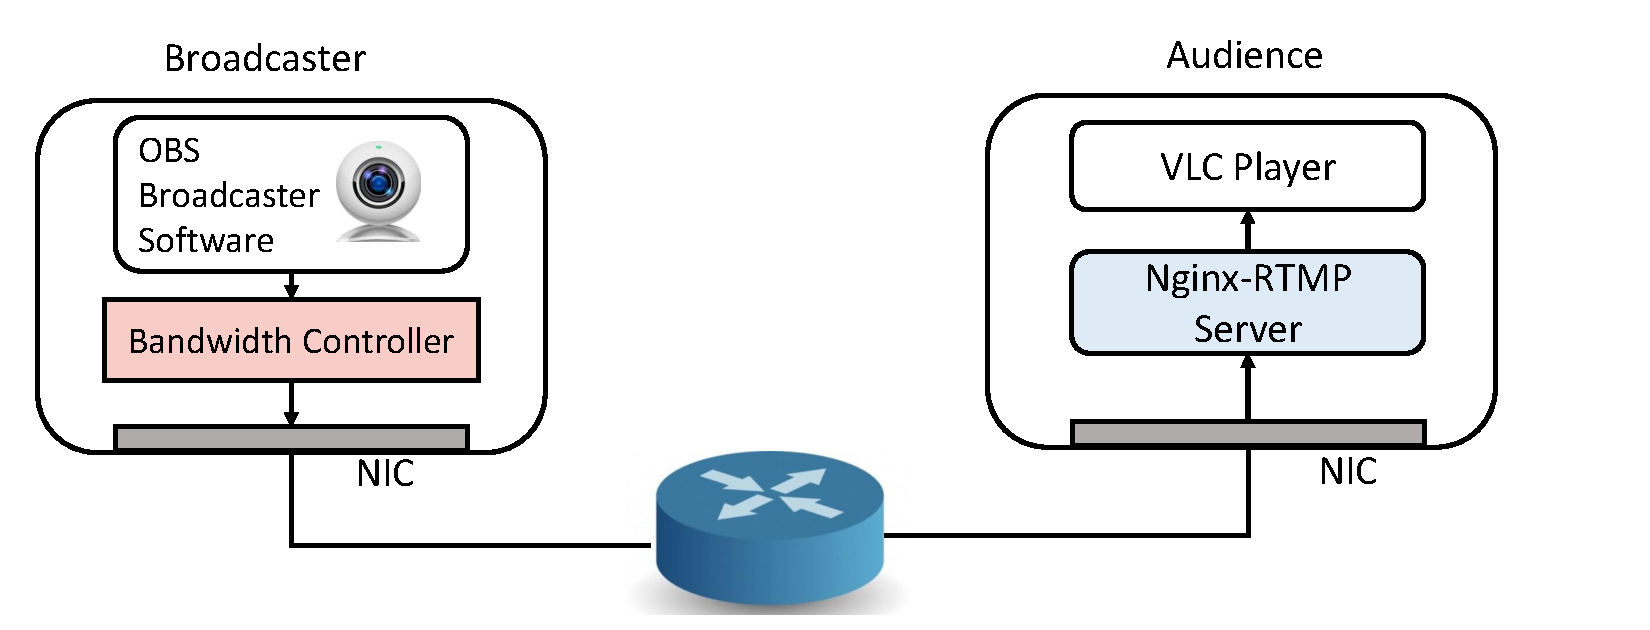
\includegraphics[width=0.8\textwidth]{setup}
  \caption{实验设置}
  \label{fig:setup}
\end{figure}

\textbf{实验设置} 我们搭建的直播传输架构如图~\ref{fig:setup}所示,包含两个主机和一个路由设备。 两端的设备(主播端和观众端)都配备有两个CPU,6G内存,设备的网卡带宽为100Mbps,他们通过中间的交换机连接在一起。主播端配备有摄像头,通过OBS软件将摄像头抓取的内容上传至直播服务器。OBS是一个开源的商业级直播软件~\cite{OBS},斗鱼和Twitch都将OBS作为推荐使用的直播软件。另外,OBS主要是使用RTMP协议来完成视频的上传。我们在主播端实现了一个带宽控制的模块,能够实时模拟无线环境的网络带宽变化。带宽控制模块在Linux系统下用Linux系统自带的tc模块实现,在Windows系统下则用dummynet~\cite{dummynet}来实现。在观众端,我们使用nginx的nginx-rtmp模块搭建了一个RTMP服务器,用来接收主播端上传的视频。另外,我们用VLC播放器去播放RTMP服务器接收到的直播视频流。

\subsection{案例分析:带宽抖动导致传输质量差}
为了尽量真实地模拟无线网络环境,我们使用真实的数据记录去控制实验的带宽变化。当用户通过移动设备浏览亚马逊网站时,每隔5秒给服务器发送探测到的实时带宽信息,我们以这种方式获取数据记录。我们将整个直播过程切分为多个5秒的时间段,将每个时间段内发送的所有数据报文聚合在一起,然后计算每个时间段内的总数据量,之后根据带宽的实际数值去控制主播端的网络带宽。我们选取其中260秒的记录作为具体案例,这一段数据的平均带宽在3300kbps以上。 实验一开始我们把直播的码率设为3300kbps,低于平均码率,这是为了防止整个过程码率始终低于平均值,无法判断出直播平台应对网络抖动的能力。启动OBS,上传摄像头抓取到的视频;与此同时,在观众端启用tcpdump去实时抓取报文。整个过程实时的吞吐量结果如图~\ref{fig:case_study}所示,为了更清晰的展示实验结果,我们把数据记录分为两个部分,0-140秒以及120-260秒。

\begin{figure}[h]
  \centering%
  \begin{subfigure}{0.49\textwidth}
    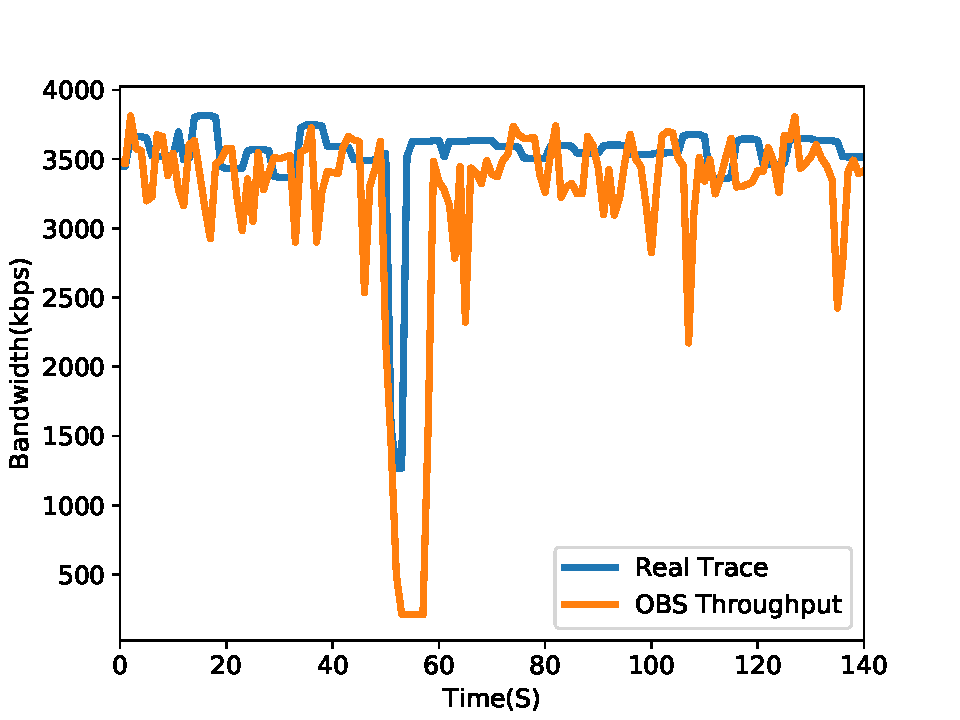
\includegraphics[width=\textwidth]{case_study_throughput_a}
    \caption{0-140s的吞吐量}
    \label{fig:case_study_a}
  \end{subfigure}%
  \hfill
  \begin{subfigure}{0.49\textwidth}
    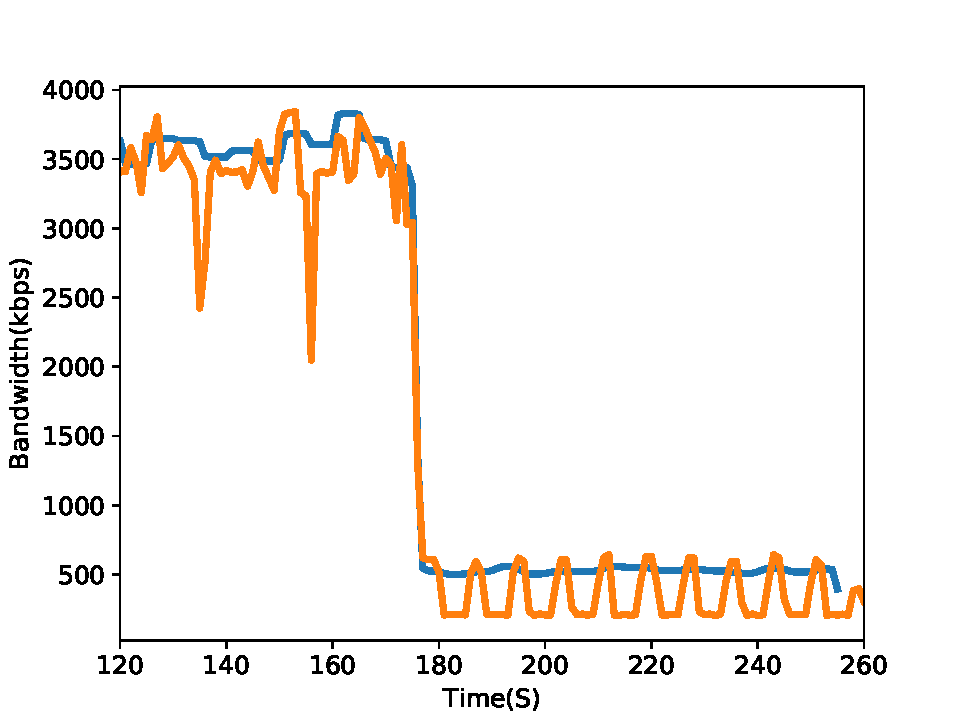
\includegraphics[width=\textwidth]{case_study_throughput_b}
    \caption{120-260s的吞吐量}
    \label{fig:case_study_b}
  \end{subfigure}
  \vspace{0.1in}
  \caption{无线网络环境下直播应用的吞吐量}
  \label{fig:case_study}
\end{figure}

仔细观察上述实验图,我们可以得出以下两个结论。(1)从图~\ref{fig:case_study_a}我们可以看出,大部分时间里,主播端的实际带宽一直紧紧跟随控制带宽发生变化。然而,在50秒附近,带宽大幅度衰减,低于初始的码率,维持在1500kbps左右,这种情况维持了2秒钟。此时,真实的数据吞吐量基本降为0,这一现象维持了8秒钟,从50秒到58秒。这是一种不正常的现象,2秒的网络抖动导致了直播流8秒的吞吐量下降。(2)从图~\ref{fig:case_study_b}可以看出码率固定的策略并不能有效的应对长时间的带宽变化。0-180秒期间带宽始终是充足的,高于实时的码率3300kbps,但是180秒之后带宽急剧变化,下降到500kbps左右,这个过程持续了80秒的时间。在这期间主播端显示,发生了大量的丢帧。在网络很差的环境下,OBS主播端依然维持在默认的码率值,但实时带宽远远小于码率值,网络无法将产生的视频流推送出去,这个策略显然不能达到很好的效果。

\subsection{带宽抖动的普遍性}
\begin{figure}[h]
  \centering%
  \begin{subfigure}{0.49\textwidth}
    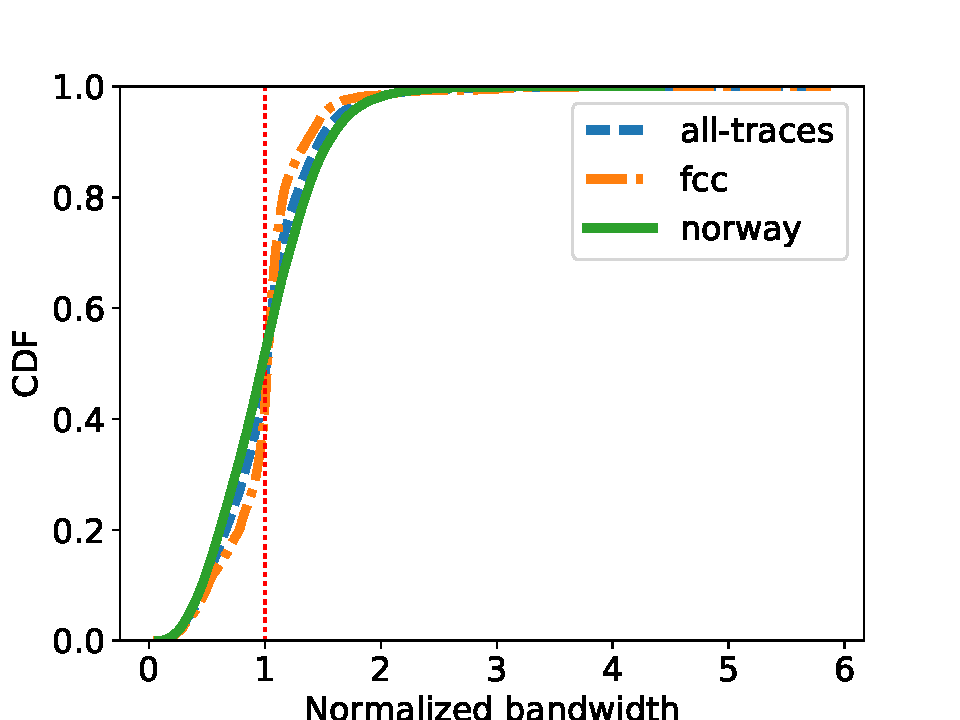
\includegraphics[width=\textwidth]{trace}
    \caption{归一化带宽累计分布函数}
    \label{fig:trace}
  \end{subfigure}%
  \hfill
  \begin{subfigure}{0.49\textwidth}
    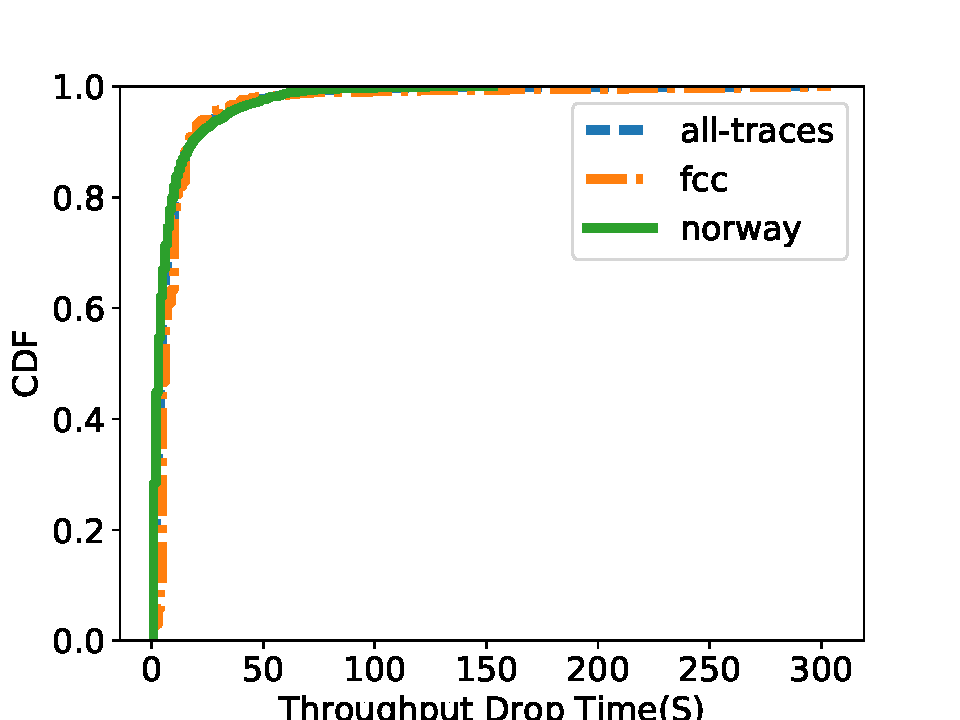
\includegraphics[width=\textwidth]{trace-down}
    \caption{带宽抖动时长分布}
    \label{fig:trace_down}
  \end{subfigure}
  \vspace{0.1in}
  \caption{无线网络环境的带宽分布}
  \label{fig:case_study}
\end{figure}

为了评估无线网络环境下带宽抖动发生的频率,我们将两个真实的大规模公开数据集组合起来,以便数据分析。两个公开的数据集分别是Wifi网络环境下的FCC数据集~\cite{FCC}和移动网络环境下的HSDPA数据集~\cite{riiser2013commute},其中每个数据记录的持续时长为320秒,两个数据集的总共持续时间为30多个小时。针对每一条数据记录,我们把平均带宽作为单位数,去归一化每个数据记录的所有数据点,总的cdf图如图~\ref{fig:trace}所示。有50\%左右的时间,记录的数值小于平均带宽,这意味着对于一个10秒的带宽记录来说,有5秒的时间,实时带宽会低于平均值。20\%的情况下记录的数值只有平均值的一半。总的CDF分布图表明在真实网络世界中,带宽波动出现的很频繁。

为了进一步说明每次带宽抖动持续的时间,我们画了一张带宽抖动时长分布的CDF图~\ref{fig:trace_down}。带宽抖动时长是通过计算带宽在平均值以下的持续时间。大约20\%的网络抖动其持续时长多于10秒,有些甚至持续数百秒。另外,我们在上面的两张图中还分别画出了FCC数据集和HSDPA数据集的带宽分布和抖动时间分布,两个数据集单独的分布和整体分布相同,差别不大。

\subsection{商业平台验证}

\begin{figure*}[htb]
  \centering%
  \begin{subfigure}[b]{\textwidth}
    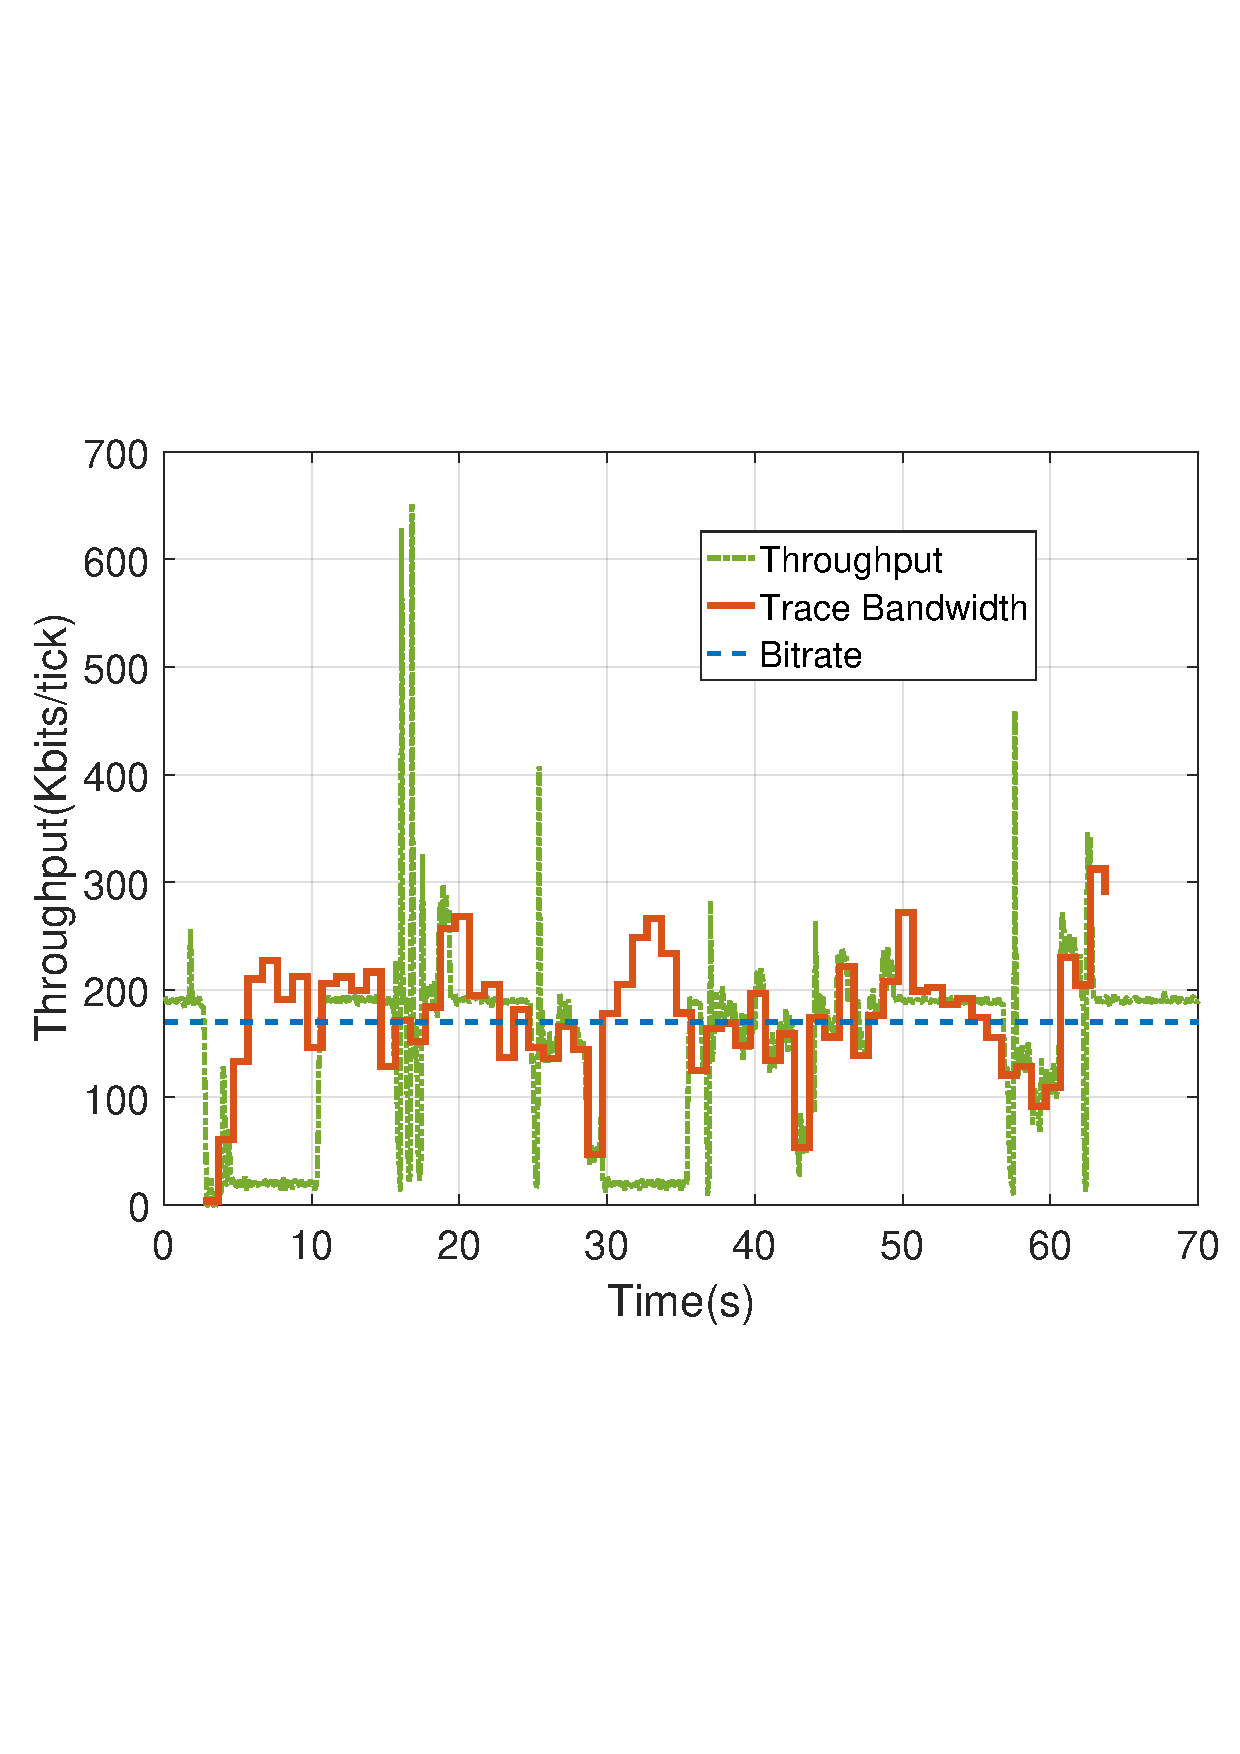
\includegraphics[width=0.46\textwidth]{obs_douyu}
    \hfill
    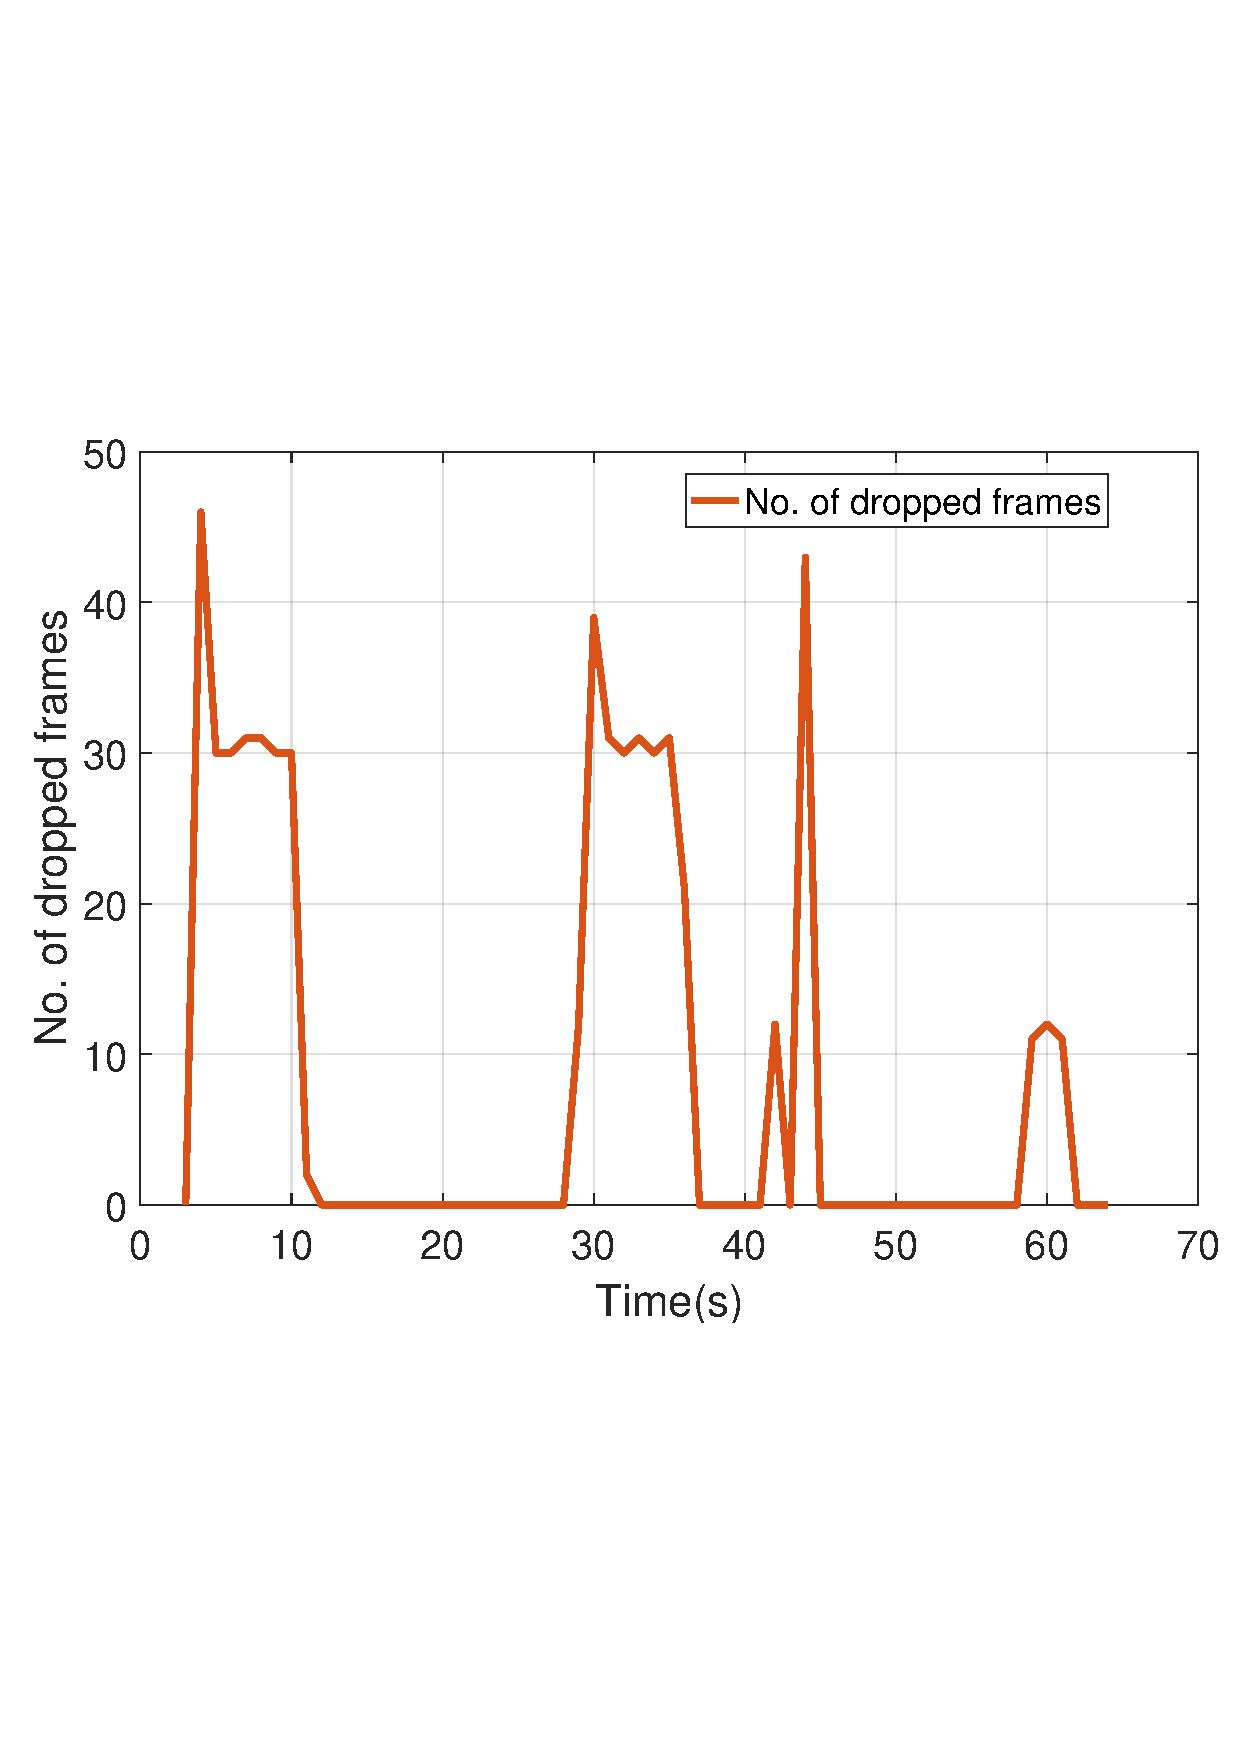
\includegraphics[width=0.46\textwidth]{obs_douyu_drop}
    \caption{OBS推流至斗鱼服务器的吞吐量和丢帧}
    \label{fig:obs_douyu}
  \end{subfigure}
  \vfill
  \vspace{0.2in}
  \begin{subfigure}[b]{\textwidth}
    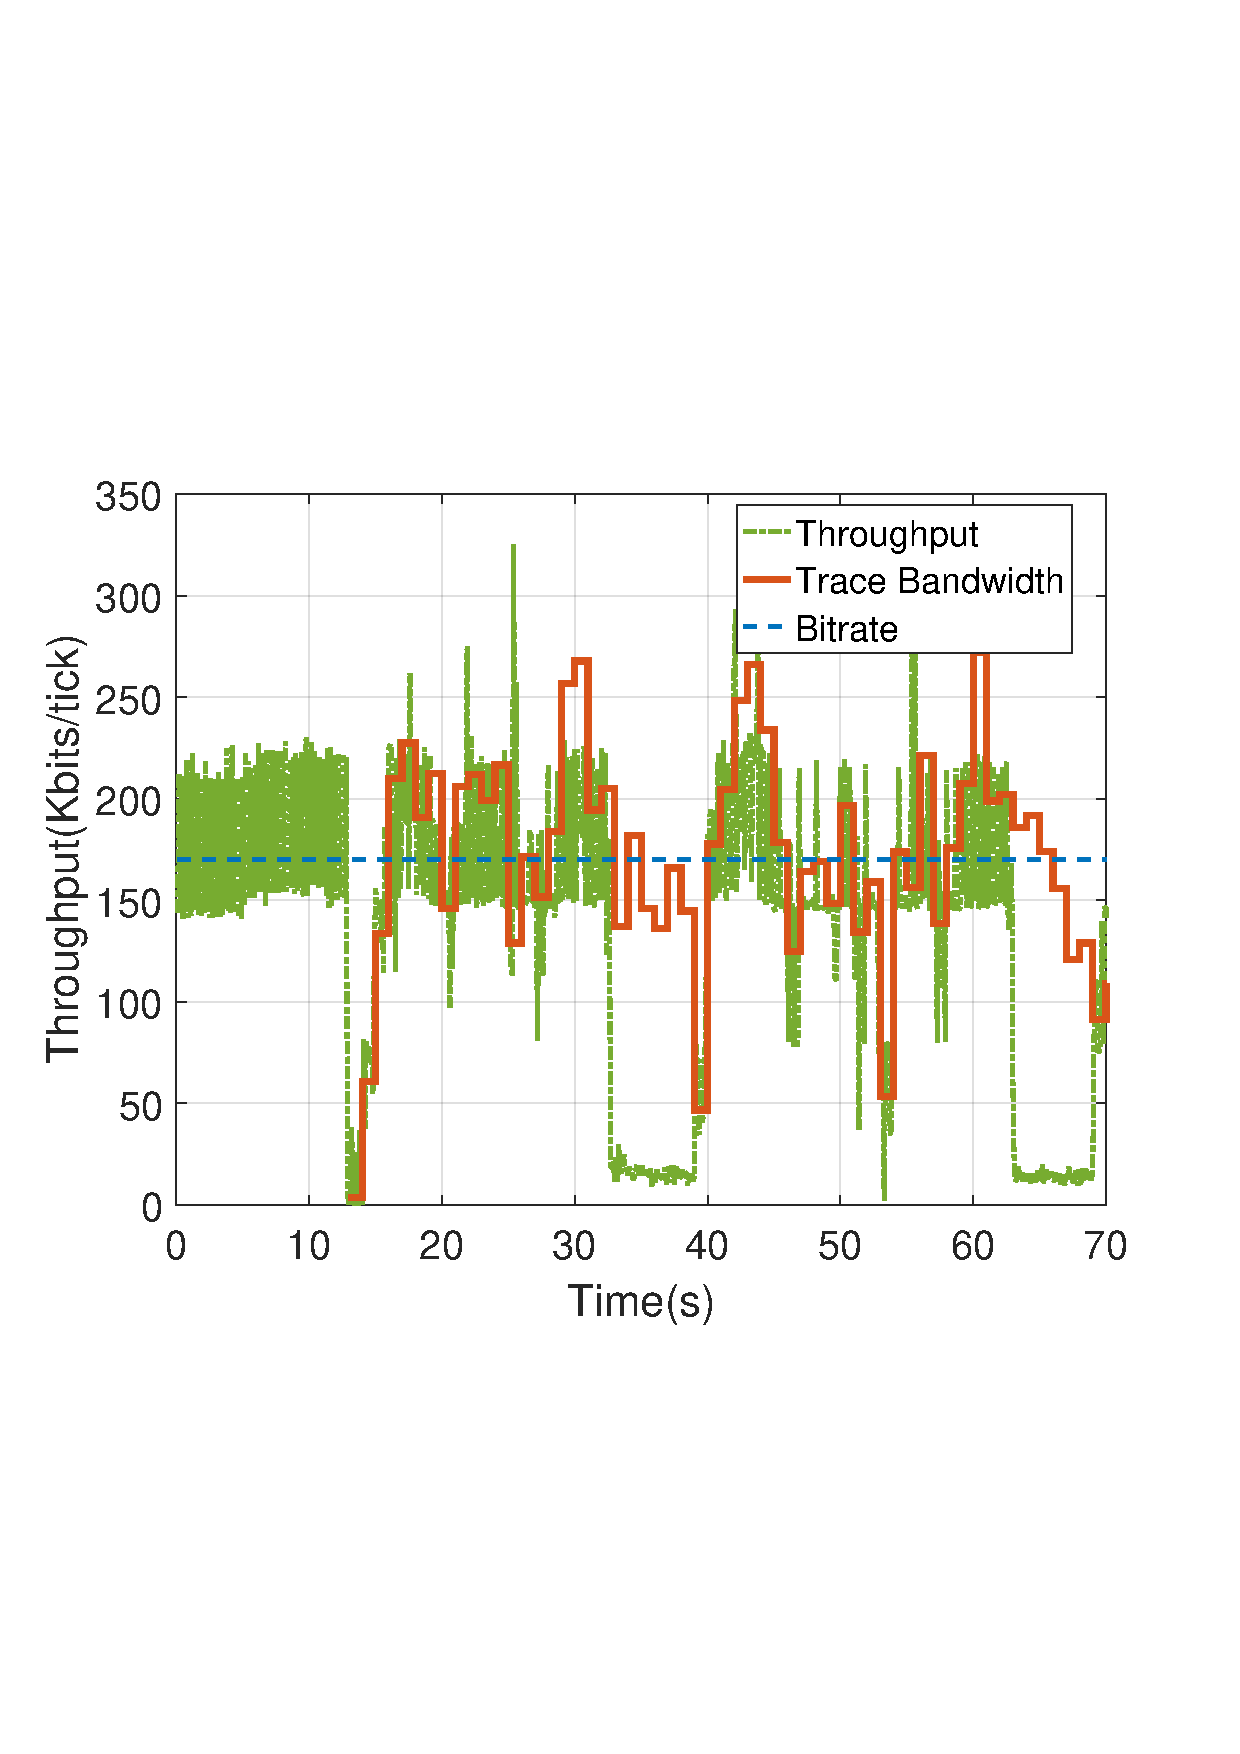
\includegraphics[width=0.46\textwidth]{douyu}
    \hfill
    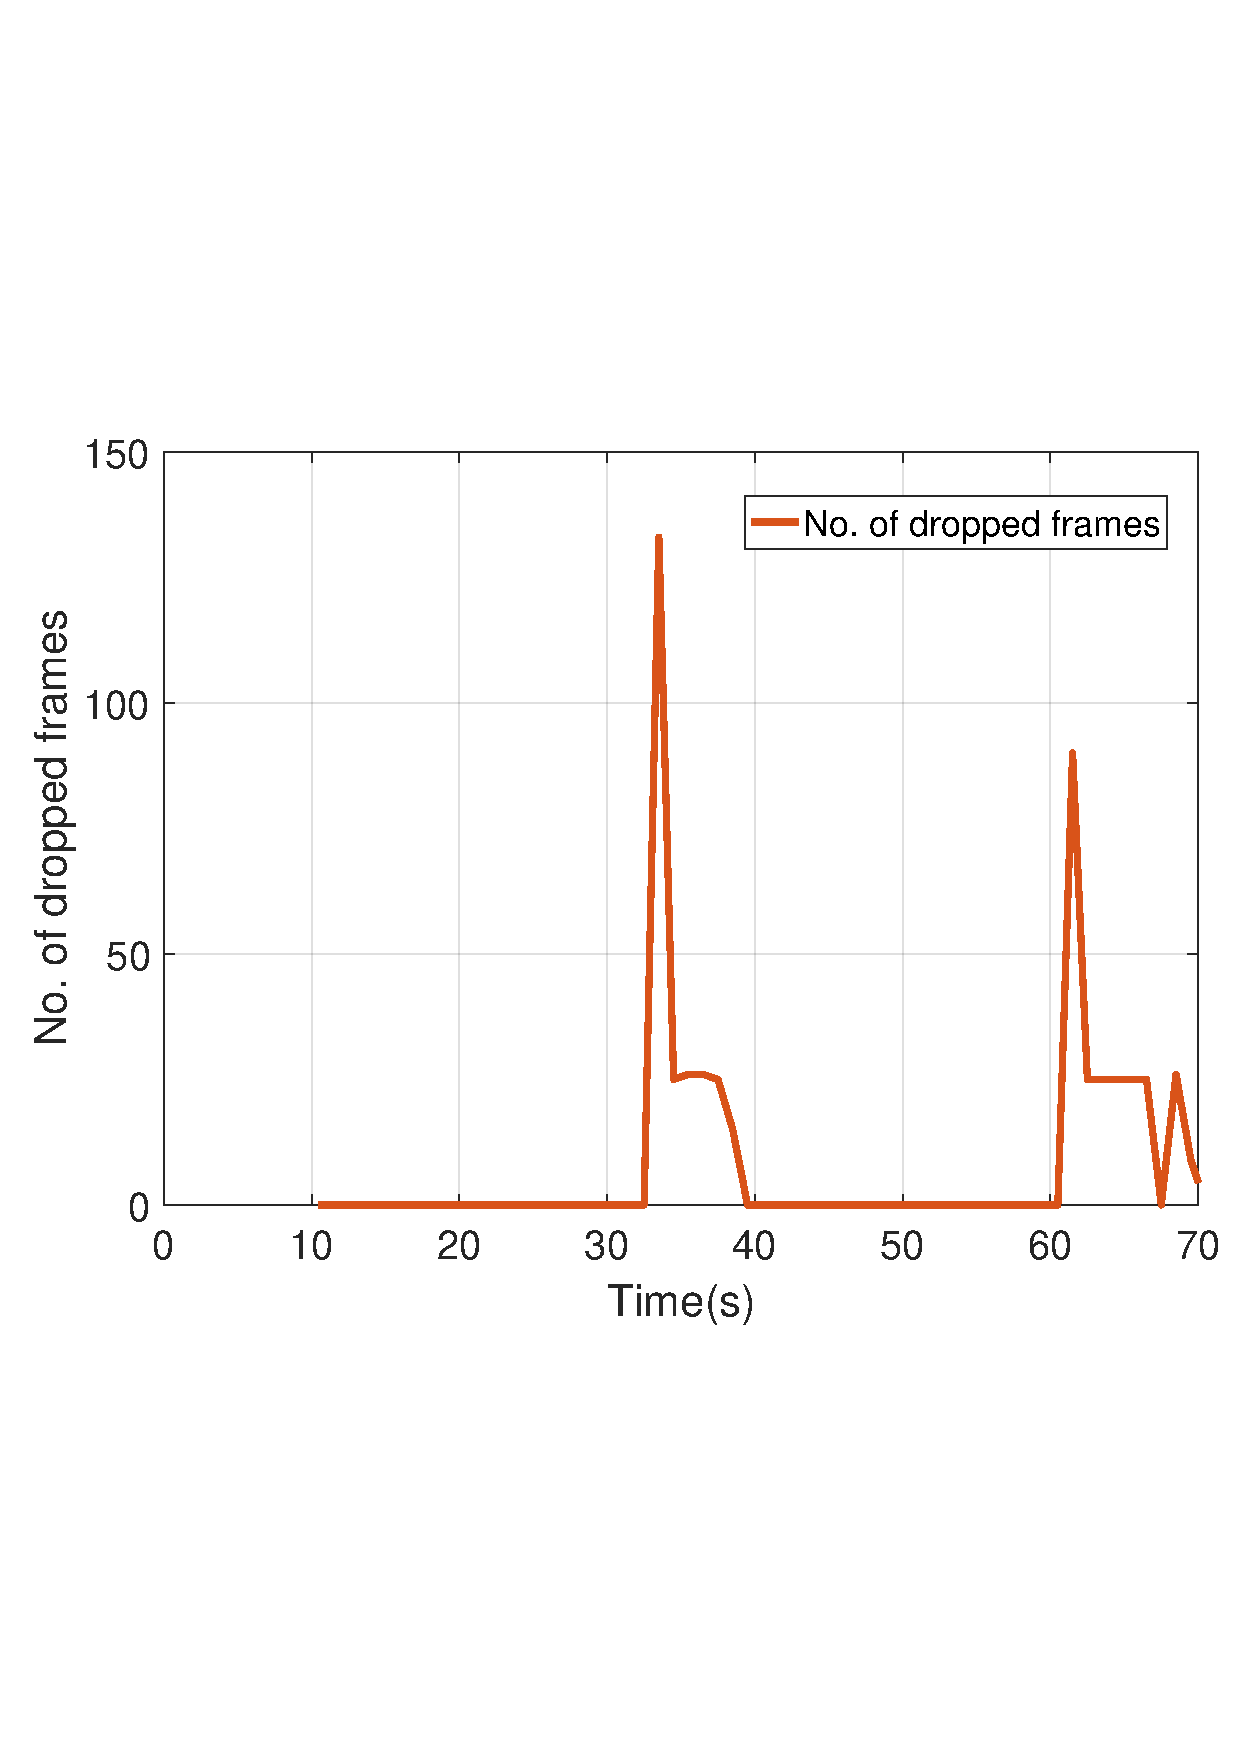
\includegraphics[width=0.46\textwidth]{douyu_drop}
    \caption{斗鱼主播工具推流至斗鱼服务器的吞吐量和丢帧}
    \label{fig:douyu}
  \end{subfigure}
  \vfill
  \vspace{0.2in}
  \begin{subfigure}[b]{\textwidth}
    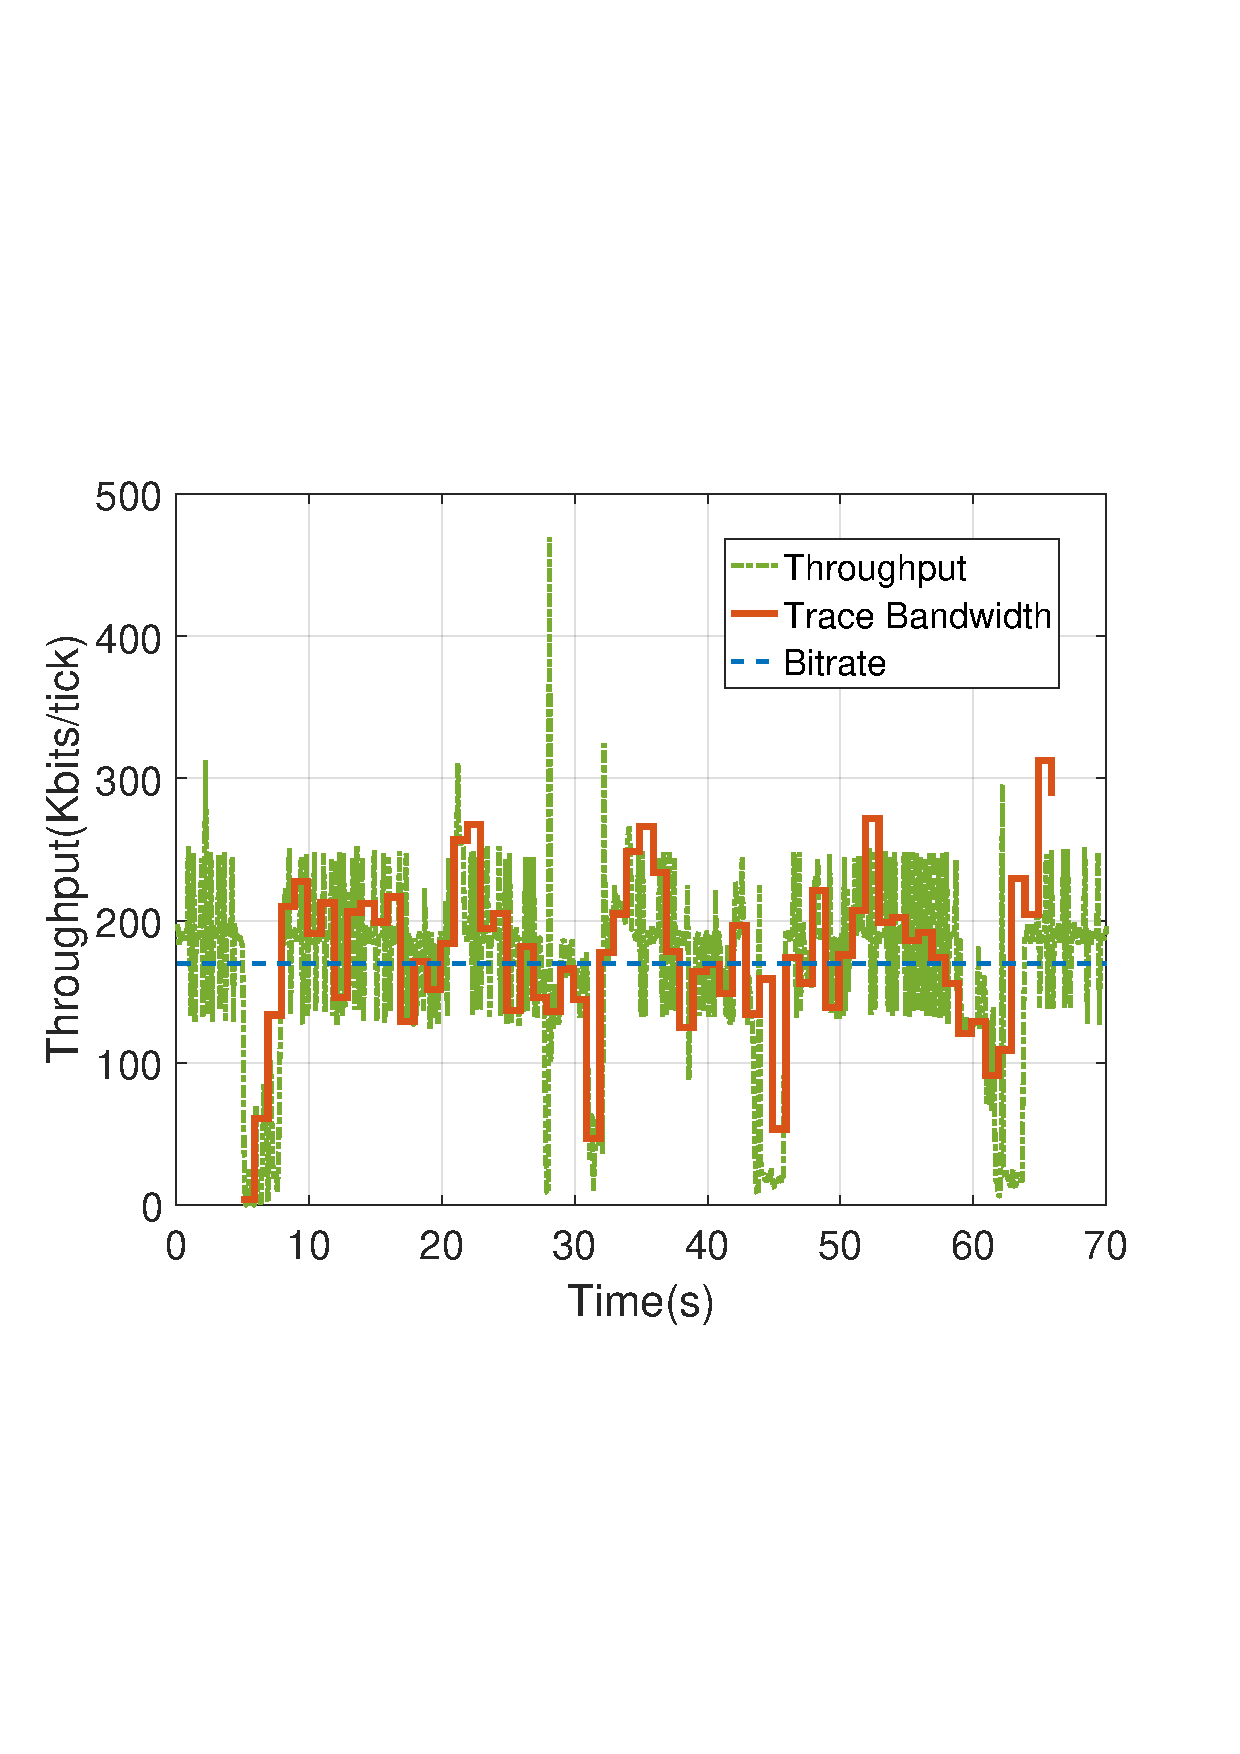
\includegraphics[width=0.46\textwidth]{obs_twitch}
    \hfill
    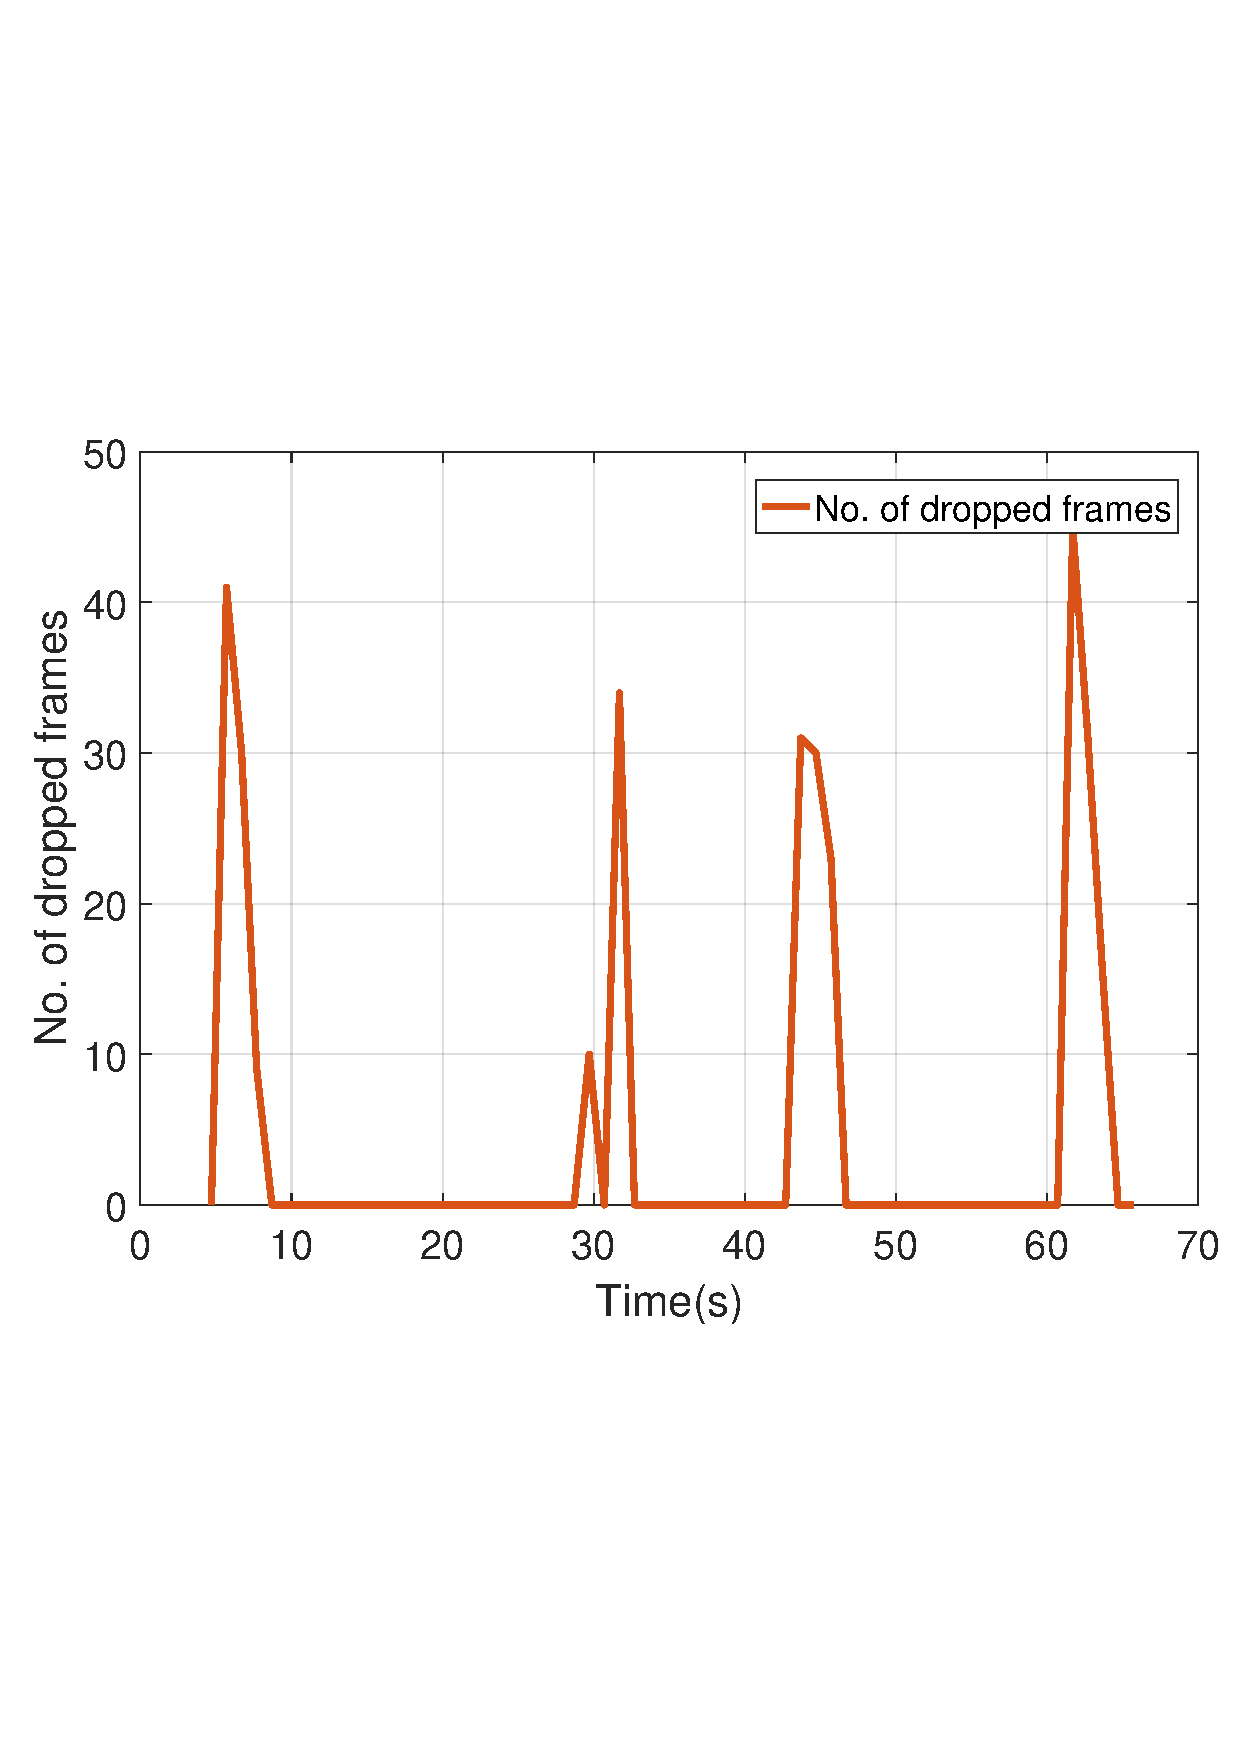
\includegraphics[width=0.46\textwidth]{obs_twitch_drop}
    \caption{OBS推流至Twitch服务器的吞吐量和丢帧}
    \label{fig:twitch}
  \end{subfigure}
  \caption{商业平台验证实验}
  \label{fig:commerical_application}
\end{figure*}


经过对真实网络环境的分析,我们发现在无线网络状况下,带宽抖动发生的次数较为频繁,且每次带宽抖动都会持续一定的时长。通过对开源直播软件OBS的测量实验发现,带宽抖动情况下OBS会遇到视频质量下降的问题。为了验证流行的商业平台上是否存在相同的问题,我们选择了几个交互直播的商业平台去重复上述的实验。分别是OBS作为主播端推流到斗鱼服务器,斗鱼主播工具推流到斗鱼源服务器,OBS推流到Twitch的服务器。三组实验所用的带宽数据相同,初始的码率选择也相同,为1700kbps,数据记录的平均可用带宽高于初始码率。在实验过程中实时带宽偶尔会低于初始码率,我们用tcpdump去实时抓取真实的带宽。图~\ref{fig:commerical_application}分别表示了三种实验环境下实际吞吐量的时序图,以及总丢帧数图。另外,表~\ref{tb:drop}的前三行记录了每组实验的总丢帧数。

\begin{table}[h]
\centering
\caption{不同实验配置下的丢帧数}
\label{tb:drop}
{\setlength{\tabcolsep}{4pt}
\begin{tabular}{|c|c|c|l|}
\hline
\textbf{实验组} & \textbf{实验配置} & \textbf{上传失败时长(秒)} & \textbf{上传失败比例(\%)}   \\ \hline
\multirow{3}{*}{Figure ~\ref{fig:commerical_application}}&  Obs主播端推流到斗鱼服务器               & 18.1         & 30.2\%                           \\ \cline{2-4}
& Obs主播端推流到twitch服务器              & 9.9        & 16.3\%    \\ \cline{2-4}
& 斗鱼主播工具推流到斗鱼服务器            & 16.6      & 27.2\% \\ \hline
\multirow{4}{*}{Figure 3.7} & Obs主播端推流到斗鱼服务器            & 93.1      & 37.2\%     \\ \cline{2-4}
& Obs主播端推流到twitch服务器             & 79.3      & 31.7\%  \\ \cline{2-4}
& 斗鱼主播工具推流到斗鱼服务器              & 66.67         & 26.7\%  \\ \hline
\end{tabular}}
\end{table}

对比不同商业平台的测量结果,我们发现之前在OBS平台观察到的应用层上传暂停现象普遍存在,所有的商业平台都出现了类似的现象。大部分情况下,实际带宽紧跟着数据记录变化。OBS推流至斗鱼服务器时现象出现在30-36秒,斗鱼主播工具推流到斗鱼服务器的情况下发生在32-39秒,OBS推流端推流至Twitch服务器时现象发生在43-45秒。我们观察三个时间段内的丢帧数,发现丢帧数一直维持在一个很高的数值。另外,我们从图中发现应用层放大现象的出现和带宽降低的幅度没有必然联系。例如,图~\ref{fig:obs_douyu}中,带宽在30秒时剧烈下降,降低为原来带宽的17\%,此时出现了应用层放大效应。但在图~\ref{fig:douyu}中,32秒时带宽轻微地下降,降低为原来的85\%左右,轻微的带宽降低也触发了应用层的放大效应。由此可以得出结论,应用层放大效应的出现并不取决于带宽降低的幅度。另外一个发现是,放大现象导致的丢帧持续时间在不同商业平台上也各不相同:斗鱼平台上有多于5秒的丢帧,而Twitch平台上只出现了2-3秒的丢帧。表~\ref{tb:drop}中显示,斗鱼作为RTMP服务器时,上传失败的比例在30\%附近,Twitch作为服务器时,上传失败的百分比只在16\%附近,进一步验证了不同商业平台的丢帧时间不同。总之,上述的实验结果表明商业平台的直播端也不能够有效的解决短时间的带宽下降。

\begin{figure}[htb]% use float package if you want it here
  \centering
  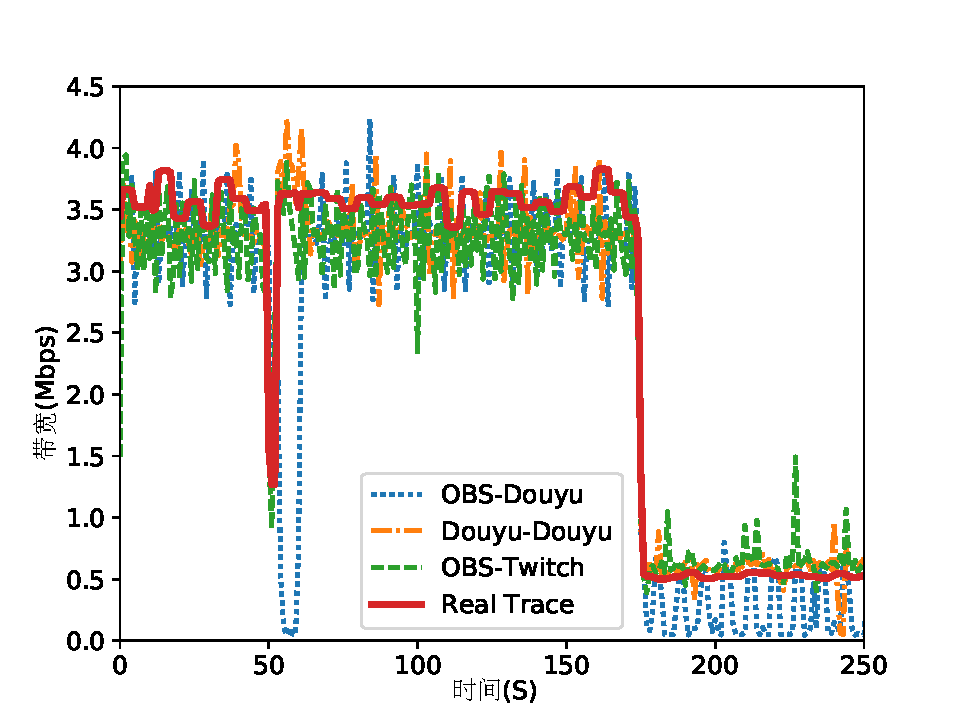
\includegraphics[width=0.7\textwidth]{vary-bandwidth}
  \caption{长时间带宽抖动状况下的吞吐量}
  \label{fig:vary-bandwidth}
\end{figure}

除了短时间带宽下降的实验之外,我们还验证了长时间带宽下降时商业平台的性能表现,如图~\ref{fig:vary-bandwidth}所示。与上面的实验相同,我们选取的初始码率3300kbps小于平均带宽,实验开始的一段时间里,实时带宽一直高于初始码率,主播端上传的视频很流畅。但在180秒之后带宽开始急剧的下降,降低到500kbps附近,实验期间我们持续观察码率变化,发现所有三组实验环境的码率依然保持不变,均维持在初始码率。但180秒之后,实时的码率大于带宽,视频数据产生的速度远远大于网络容量,观测到了大量的丢帧现象。OBS推流至斗鱼服务器的这组实验表现最差,甚至都没有充分利用带宽资源。尤其是180秒到250秒期间,这组实验的实时带宽在网络容量和零之间来回振荡。而观察其他两组实验,虽然整个过程中真实带宽紧跟网络容量变化,但180秒之后主播端一直在持续不断的丢帧。表~\ref{tb:drop}的后面三行记录了总共的丢帧数据,三组实验的上传失败百分比都很高,进一步说明了现有的商业平台处理长时间带宽下降的能力非常的有限。总的来说,现有的商业平台不能有效解决长时间带宽下降的情境下丢帧的问题。

\section{本质原因追溯}

\begin{figure}[htb]% use float package if you want it here
  \centering
  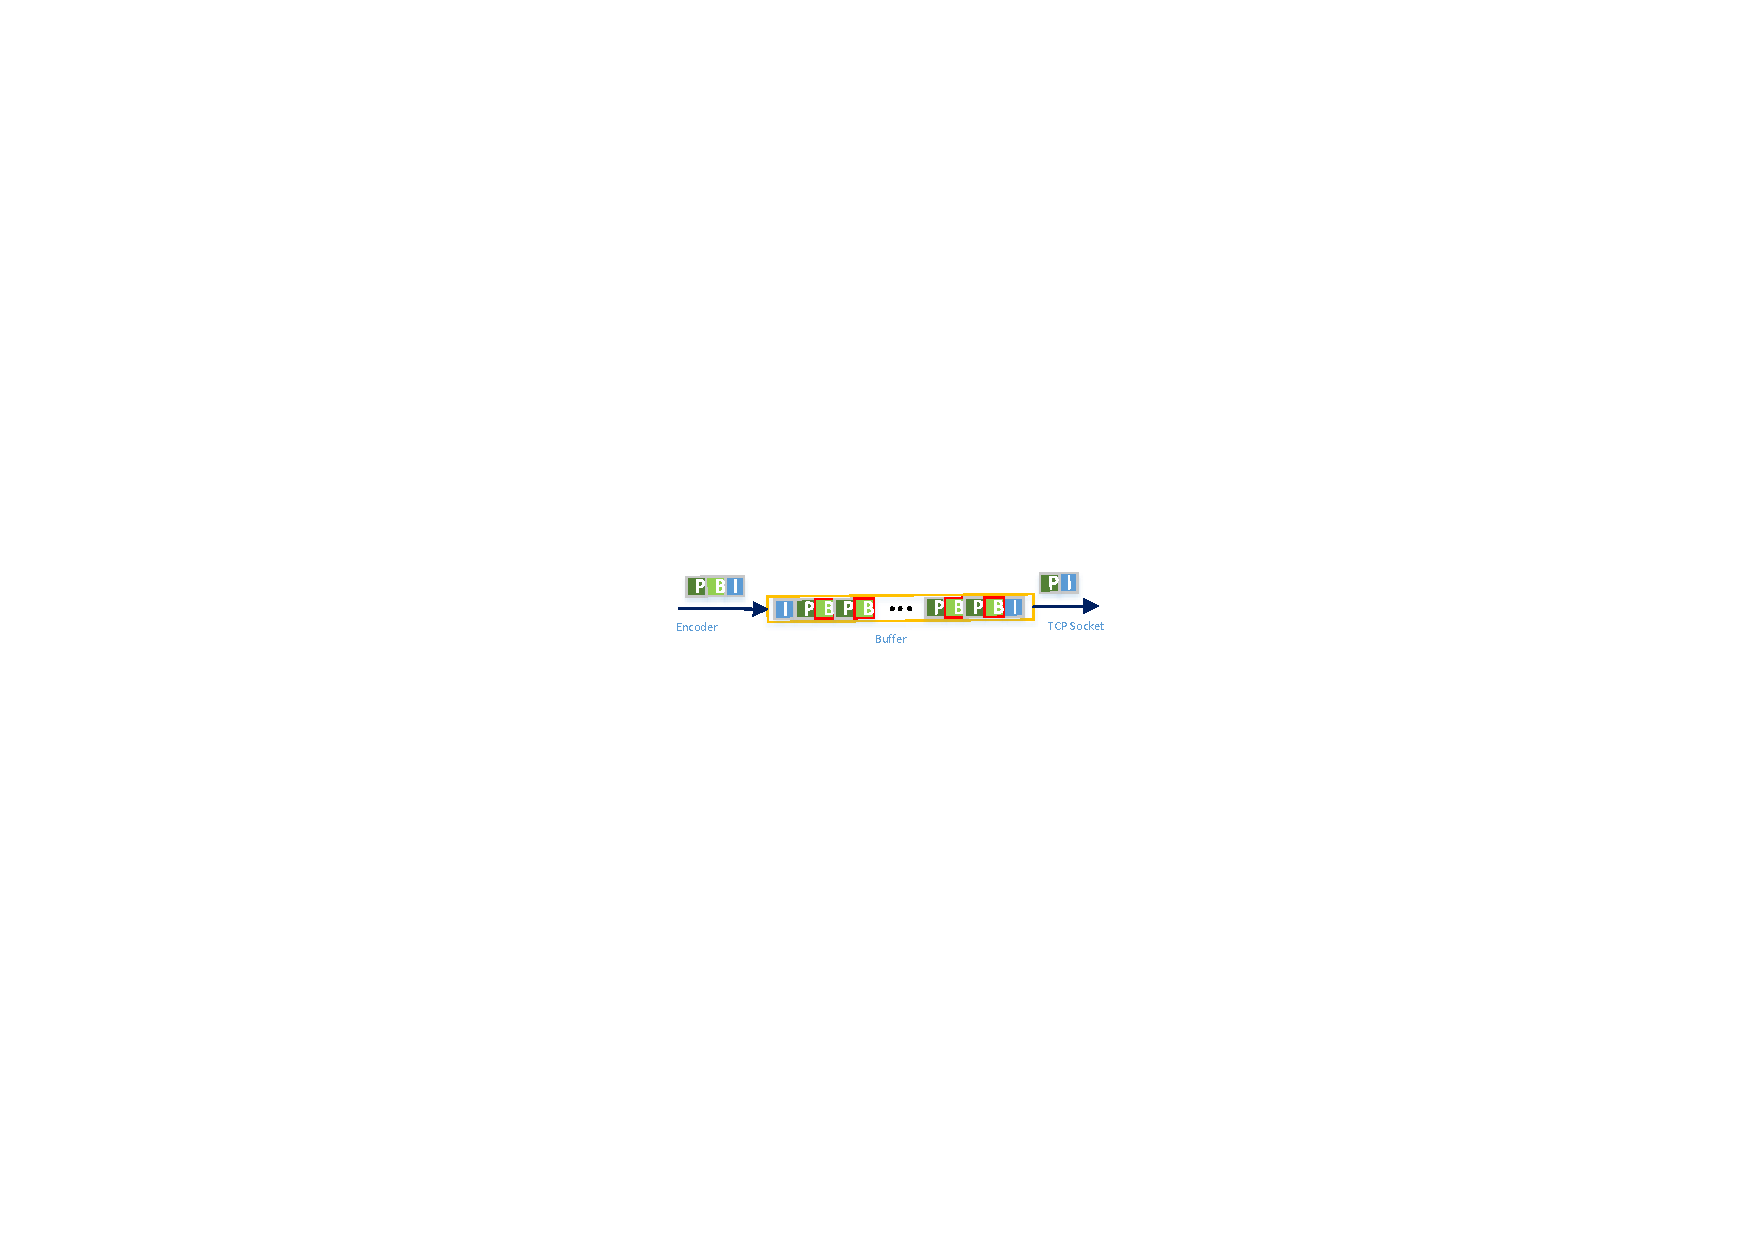
\includegraphics[width=0.8\textwidth]{drop}
  \caption{视频帧队列示意图}
  \label{fig:drop}
\end{figure}

无论是有线网络环境还是无线网络环境,网络带宽抖动都时有发生。为了应对可能出现的带宽抖动,主播端应该会维护一个队列来存储等待发送的视频帧数据。主播端的视频帧队列的示意图如图~\ref{fig:drop}所示。主播端通过摄像头实时抓取画面,之后将抓取的画面送入编码器,编码成H264格式的视频帧;编码完成后的视频帧被编码器释放出来,进入视频帧队列排队等待被发送。同时发送数据的进程从队列中顺序取出一个视频帧,将它通过TCP蹭的socket端口发送到网络中去,整个视频编码发送的过程便是这样。如果网络状况不好,网络容量低于视频数据产生的速率,数据发送的进程会被堵塞住,视频帧队列累积到一定程度会超出最大空间容量的限制,之后新产生的视频帧直接被丢弃,不再纳入帧队列,于是发生了丢帧现象。另外,视频帧队列里的数据帧也会因为超出最大容量的限制,而有可能会丢弃。

\begin{figure}
\centering
%\small
{\setlength{\tabcolsep}{4pt}
\begin{tabular}{|r||ccccccccc|cc|}
\hline
帧类型       & I & B & B & P & B & B & P & B & B  & I  & ... \\ \hline
播放顺序   & 1 & 2 & 3 & 4 & 5 & 6 & 7 & 8 & 9  & 10 & ... \\ \hline
编码顺序 & 1 & 3 & 4 & 2 & 6 & 7 & 5 & 9 & 10 & 8  & ... \\
\hline
\end{tabular}}
\caption{H.264帧的编码顺序和播放顺序}
\label{fig:frame-order}
\end{figure}

丢帧现象产生的主要原因是网络堵塞。但大量的测量实验发现,丢帧可能还会在应用层造成放大效应。为了找到问题发生的根本原因,我们通过追溯开源直播软件OBS的源码,发现短时间的带宽抖动导致的丢帧放大效应主要是由于视频帧之间存在依赖关系。按照H264的编码标准,一段视频最后会被编码成一个图片组,称之为一个GoP(Group of Pictures)。编码协议规定,每个图片组的第一帧应保持原图不变,这一帧称为I帧,也称之为关键帧。P帧是利用前面已经编码的图像作为参考图像进行预测生成的,已经编码的图像包含前面的I帧和P帧;B帧则是一种双向预测,根据邻近的I帧和P帧产生。表~\ref{fig:frame-order}给出了一系列连续的视频帧的示意图,按照播放顺序展示。表中可以看出,视频帧的编解码的顺序和最后实际播放的顺序并不一定一致。考虑到一个GoP里视频帧之间的依赖关系,当一组GoP中间的P帧被丢弃的话,这个P帧之后所有的P帧和B帧都不能够正常解码。因此,如果网络带宽发生一次小抖动,导致一组GoP的中间或者开头出现丢帧现象,这个GoP剩余的帧都会被主播端丢弃,因此即使传输成功,也无法正常解码。这个原因导致我们在应用层观测到了放大效应,2秒的带宽抖动带来5-6秒的主播上传暂停。

\begin{algorithm}[htb]
\caption{OBS默认丢帧算法}
\label{alg:obs-drop}
{\bf Require:} timespan:队列时间长度;dropPFrame:和P帧相关的丢帧优先级;dropBFrame:和B帧相关的丢帧优先级;bandwidth:每个时隙的带宽
\begin{algorithmic}[1]
\State T1 := 0.9秒,T2:=0.7秒,timespan :=0
\If{新产生的帧是I帧}
\State dropPFrame := False, dropBFrame :=False
\State \Call{入队}{视频帧队列, 新产生的帧}
\State timespan:= timespan + 1
\EndIf
\If{新产生的帧是P帧}
\If{dropPFrame or timespan $>$ T1}
\State \Call{丢弃}{新产生的帧},丢弃所有的I帧和P帧
\State timespane := timespan - 丢弃的时长
\Else
\State \Call{入队}{视频帧队列, 新产生的帧}
\State timespan := timespan + 1
\EndIf
\EndIf
\If{新产生的帧是B帧}
\If{dropBFrame or timespan $>$ T2}
\State \Call{丢弃}{新产生的帧},丢弃所有的B帧
\State timespan := timespan - 丢弃的时长
\Else
\State \Call{入队}{视频帧队列,新产生的帧}
\State timespan := timespan + 1
\EndIf
\EndIf
\State timespan := timespan - \Call{发送的时长}{bandwidth}
\end{algorithmic}
\end{algorithm}


通过分析OBS主播软件的源码,我们破解了它的帧队列管理算法,如算法~\ref{alg:obs-drop}所示。OBS默认的丢帧算法引入了三个变量,P帧和B帧相关的丢帧优先级以及队列时间长度。丢帧优先级的设置是为了避免无效传输一些无法解码的视频帧,增加对网络带宽的利用率;队列时间长度表示队列中最旧的帧和当前时间刻度之间的差值。当主播端发生丢帧时,丢帧优先级被置为True,视频队列停止接收GoP中剩余的其他帧。一开始,所有的丢帧优先级都会被初始化为False。当一个新的视频帧产生时,先判断该帧是否是I帧,如果是,加入视频帧队列,并将所有的丢帧优先级赋值为False。因为I帧标志着一个新的GoP的开始,所以所有的丢帧优先级都被赋为初始值,同时,将队列的时间长度增加一个视频帧的时长。如果新产生的视频帧是P帧,判断队列时间长度是否小于0.9秒,以及P帧对应的丢帧优先级是否为True。如果队列时间长度大于0.9秒,或者P帧对应的丢帧优先级为True,则丢弃当前帧,B帧和P帧的丢帧优先级都被设为True。而且如果时间长度多余0.9秒,丢弃队列里所有的P帧和B帧,时间长度减去队列中丢弃帧的时间长度。上述两个条件均不满足的话,将新产生的P帧加入视频队列,和I帧操作相同。如果新产生的帧是B帧,队列时间长度的阈值变为0.7s,其余的逻辑和P帧类似。

大量的测量表明,当直播过程中发生带宽抖动的情况时,主播端的码率依然维持在初始的码率,视频数据产生的码率远远大于可用的无线带宽容量,便会发生丢帧现象。如果丢帧时丢弃了一个GoP中位置靠前的P帧,那么为了避免传输无效视频帧,该GoP剩余的其他视频帧都将会丢弃,映射到应用层面的表现为一段时间的上传暂停,我们称之为应用层的放大效应。通过对于开源直播软件的分析,我们可以确定地说问题发生的根本原因就是由于H264编码标准使得帧与帧之间存在依赖性。

\section{本章小结}
本章通过在实验室搭建的demo平台上的测量发现,开源的直播软件OBS目前并不能有效的应对移动网络的带宽抖动。当短时的带宽抖动发生时,在OBS平台上观测到短时的抖动会在应用层引起丢帧的放大效应;而当长时间带宽下降出现时,OBS直播平台并不能有效的应对,视频帧产生的速度一直保持不变,远远超于网络容量,造成长时间的上传视频质量不高。

为了验证在现行的商业平台上是否存在相同的问题,我们选取了OBS和斗鱼主播工具作为主播端,斗鱼服务器和Twitch服务器作为接收端,去重复我们上述的实验。在商业平台上的测量结果和demo平台的结果基本一致,表明目前的商业平台也尚未能有效地应对移动网络的带宽抖动。 通过解析OBS开源软件的源码,我们发现,应用层丢帧放大效应的主要原因是由于H264的编码标准导致帧与帧之间存在依赖性,长时间的带宽降低导致视频上传受到严重影响主要是由于视频的产生速率远远高于网络带宽容量。

为了解决上述问题,我们初步提出了两个方案,增加视频队列长度以及减少关键帧间隔。初步的仿真实验结果说明,两种方案都可以减少丢帧现象的发生,但是增加视频队列长度违反了帧传输及时性的要求。这为我们之后的优化空间提供了思路,视频队列长度应该严格控制在一个合理的阈值,将帧传输的时延控制在要求的范围内。
\chapter{移动网络中主播端传输优化方案设计}

基于第三章大量的测量实验以及对于应用层丢帧放大效应的本质原因分析,我们重新思考将RTMP协议作为主播端协议时的方案设计,尝试从视频帧和GoP等三个不同的层面来定制化主播端的传输协议。首先,我们需要选择出一个合适的关键帧间隔,以减少视频帧之间的依赖性,从而缓解应用层放大效应的发生。然后,我们尝试最优化GoP内部的丢帧策略,去尽可能多地避免不必要的丢帧。前面提出的这两个解决方案协同作用,以应对短时间的带宽降低。最后,我们设计了一个GoP粒度的码率自适应算法,来缓解长期的带宽衰落所带来视频质量的下降。

\section{优化空间}
\label{sec:design_space}

丢帧问题的发生明显地降低了观众的用户体验质量,应用层的丢帧放大效应加剧了上述问题。为了缓解丢帧问题,我们首先尝试了一些较为简单直接的方案,比如增加视频队列的长度,或者缩小视频的关键帧间隔。从理论上来说,这两个方案都可以减少丢帧现象的发生。因为我们知道帧之间的依赖性由于H264的视频压缩算法导致,非关键帧都是由关键帧计算得来。关键帧之间是相互独立的,依赖性只存在在一个GoP内部。通过减少关键帧间隔,我们可以减少视频帧之间的依赖性,从而减少丢帧。举个最极端的例子,如果关键帧间隔为1帧,那么帧之间完全不存在依赖性。另外,假设在关键帧为8秒的情况下,如果在一个GoP开始时,发生了一个2秒的网络抖动,那么整个GoP都会被丢弃;但是如果8秒的关键帧间隔被修改为2秒,就只会丢弃一个2秒的GoP。丢帧现象发生的另外一个原因是待发送的视频帧数据量超出队列最大容量的限制导致溢出,那么如果我们增加视频帧队列的长度,队列溢出的阈值被相应的提高,一定程度上可以减少一些视频丢帧。

为了验证上述提出的两种方案是否切实有效,并为我们的解决方案提供优化方向,我们对两种方案做一个初步的验证。

\begin{figure}[h]% use float package if you want it here
  \centering
  \begin{subfigure}{0.49\textwidth}
      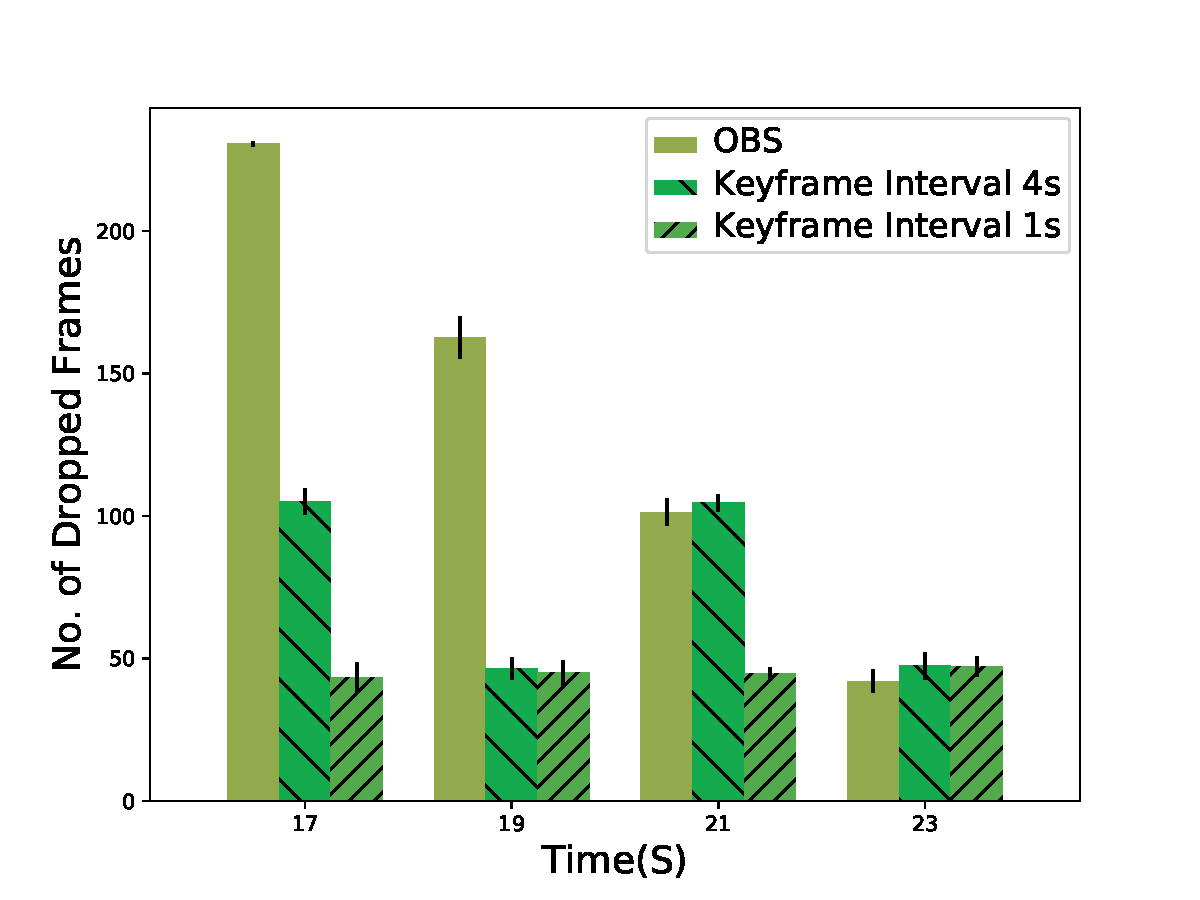
\includegraphics[width=\textwidth]{eval_IframeInterval_drop}
      \caption{不同关键帧间隔下的丢帧数}
      \label{fig:keyframe_drop}
  \end{subfigure}
  \hfill
  \begin{subfigure}{0.49\textwidth}
      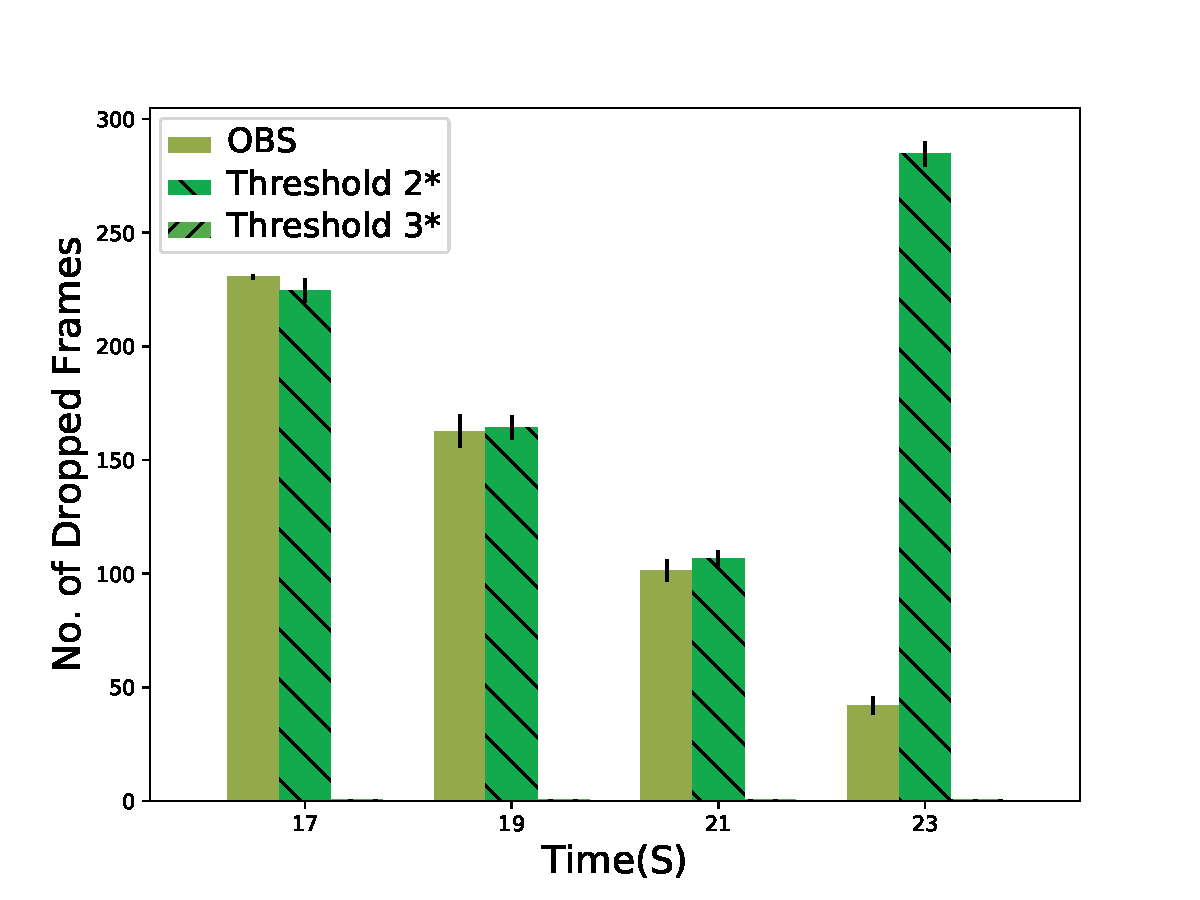
\includegraphics[width=\textwidth]{eval_threshold_drop}
      \caption{不同视频帧队列长度时的丢帧数}
      \label{fig:threshold_drop}
  \end{subfigure}
  \vspace{0.1in}
  \caption{不同编码参数下的丢帧数}
  \label{fig:prelimary_drop}
\end{figure}

\textbf{减少关键帧间隔} OBS直播软件关键帧间隔的默认值是8秒,实验中我们把关键帧间隔分别改为4秒和1秒。每次实验,我们均用OBS主播端去推流,同时为了控制变量,防止引入不必要的参数,OBS主播端推流时上传的是同一段视频。我们把OBS启动的时间定义为时间零点,为了观察关键帧对于丢帧的影响,我们分别在时间为17秒,19秒,21秒和23秒的时候断开网络连接,断开时长为2秒。丢帧的结果图展示在图~\ref{fig:keyframe_drop}中。我们可以看到,对于关键帧间隔相同的实验组来说,网络断开的时间位于一组GOP越早的时间处,丢弃的帧数则会越多。因为如果是GOP组中较早的帧,会有更多依赖于它的帧。对于默认为8秒的关键帧间隔,当断开时间分别是17秒,19秒,21秒和23秒时,丢帧数分别为238,164,105和48。因为对于关键帧间隔为8秒的情况,一个GoP的时间为16到24秒之间,17秒位于一个GoP的第1秒处,23秒的帧位于一个GoP的结尾1秒处,观察到的丢帧数也依次递增,验证了之前的理论猜想。

另外,对比在17秒时网络断开的实验组,我们发现关键帧间隔越小丢帧数减少地越明显,比如,当关键帧从8秒变到4秒再变到1秒时,丢帧数从238减到102,最后减少到46。但对于在23秒断开网络连接的实验组来说,丢帧数减少的效果并不明显。这是因为23秒处的帧在三组实验中均接近于GOP的尾部,都只有1秒时间的帧依赖于23秒处的帧。

\textbf{增加视频队列长度} OBS直播软件中默认的队列长度为,P帧0.9秒,B帧0.7秒。控制实验中我们尝试把队列长度分别改变为原来数值的2倍或3倍。原来的队列长度组合为(0.7,0.9)秒,变为2倍和3倍之后,队列阈值组合分别为(1.4,1.8)秒以及(2.1,2.7)秒。和减少关键帧间隔的实验类似,我们重复上面两组推流过程,同时记录下来每次实验的丢帧数,最后的统计结果展示在图~\ref{fig:threshold_drop}中。当队列长度增加为原来的2倍时,丢帧数并没有减少,在17秒,19秒和21秒的情况下,丢帧数基本保持不变。另外,图中可以看出在23秒时断开网络连接,丢帧数反而呈现增加的趋势。这是因为网络断开时间为2秒钟,在23秒时断开网络,队列里会缓存着一个GoP的最后一秒视频帧以及下一个GoP的开始1秒视频帧。而且OBS的丢帧策略是一旦发生丢帧,丢弃视频队列里的所有P帧和B帧,则丢帧行为会丢弃一整组GoP加一秒的视频。但当我们把队列长度增加为3倍时,丢帧数基本减少为零,这是因为队列长度的丢帧阈值为2.9秒,远远大于网络断开的时间2秒,丢帧数因此均为0。

\begin{figure}[h]% use float package if you want it here
  \centering
  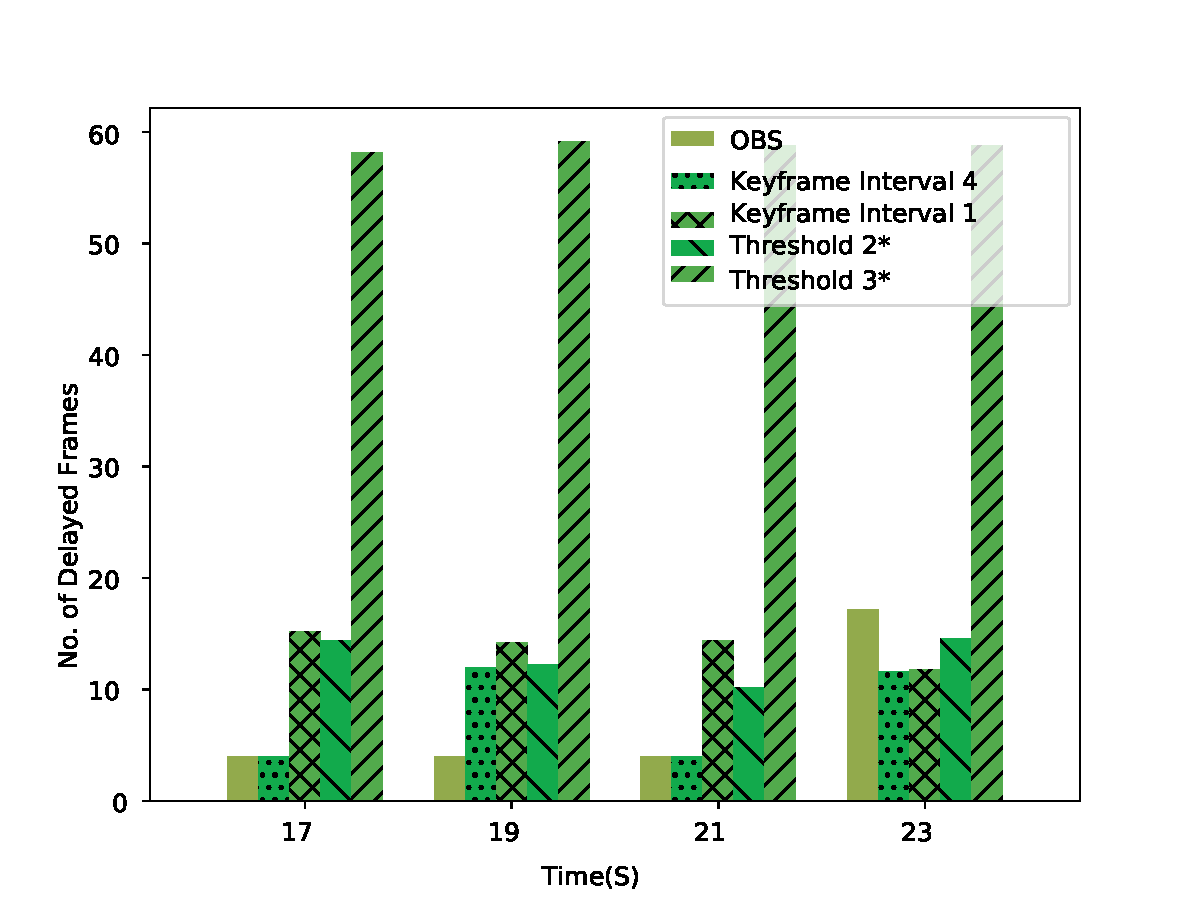
\includegraphics[width=0.7\textwidth]{timeliness}
  \caption{延迟帧的总数}
  \label{fig:timeliness}
\end{figure}

\textbf{及时性} 除了将总丢帧数作为我们的衡量指标之外,每个视频帧是否被及时的发送出去也是我们的一个重要衡量指标。为了衡量上述几组实验的及时性,我们在RTMP接收服务器处设置记录点,记录下每个视频帧的编码时间和到达时间。我们把第一个视频帧的到达时间和编码时间的差设置为0,为初始时间,记录其余视频帧和上一视频帧的编码时间和到达时间的差值,若到达时间晚于编码时间,则该视频帧被延迟了。统计总共延迟的视频帧数,并记录在图~\ref{fig:timeliness}中。从图中可以看出,当关键帧间隔变为4秒和1秒时,延迟的帧数目变化不大,维持在10帧以内,改变关键帧间隔对于及时性的影响很小。但将视频帧队列的长度增加为原来的3倍时,延迟的帧总数变为60帧左右,增加视频帧队列的长度会严重影响视频帧发送的及时性。

实验结果表明,当减少视频的关键帧间隔之后,短时间的网络带宽抖动只能引发一个相对较短时间的丢帧效应,并没有在应用层引发进一步的放大效应。增加视频帧队列的长度也可以减少丢帧的数量。这是因为增加视频队列的长度相当于提高了丢帧现象发生的阈值,从而可以减少丢帧现象的发生,因此减少一部分的丢帧。

及时性指标在直播的用户体验中也占据着重要的地位,但是上面两种方案中,增加视频队列的长度违反了及时性的要求。因此,为了满足及时性的要求,我们在之后提出的解决方案中,将视频队列长度限制在足够小的数值。之后的实验中,我们将视频队列的空间大小限制为0.9秒。另外,前面的初步验证给了我们改善视频传输质量的一些方向,比如,减少关键帧间隔。结合对于丢帧根本原因的分析,我们提出通过优化视频帧产生和传输的机制去适应变化的无线网络环境,改善用户体验质量,主要包括下面几点:

\begin{enumerate}[1)]
\item \textbf{减小视频帧之间的依赖性} 帧之间的依赖性是由于H264的视频压缩算法导致的,通过减少关键帧间隔,帧和帧之间的依赖被弱化了。然而,减少关键帧间隔会损失一定的视频质量,这个方法需要在丢帧数量和视频质量之间达到一个平衡。因为一组GoP中,一个I帧所占用的字节数很多,远远大于P帧和B帧,减少关键帧间隔,意味着同样数量的视频帧中I帧的数量增多。在同样码率的情况下,I帧数量的增多意味着每一帧分配到的数据量减少,编码器加强每一帧画面的压缩,画面的质量将会有所降低,甚至出现大的像素块;
\item \textbf{智能的丢帧策略} OBS现在的默认策略是当队列时间长度超出规定的阈值后丢弃视频帧队列里所有的P帧和B帧。目前的丢帧策略存在一定的合理性,因为如果丢弃视频帧队列中位于队列头部的视频帧,和它属于同一个GoP中剩余的其他帧也就无法解码。但是反之,如果丢弃最新的视频帧,时间较为久远的视频帧依然存在在队列中,及时性就无法保证。但是,对于队列中同时存在2个或者多个GoP的情况,一个直接的可以优化的点就是,丢弃旧的GoP的帧。这样的方法相对于OBS的默认策略会有一定的提升。设计出一个接近最优解决方案的在线的丢帧策略很重要,唯一的挑战在于帧之间存在依赖性。暴力搜索方式虽然可以找出最优解,但是由于时间复杂度太高,所以实际中并不可用;
\item \textbf{自适应码率} 图~\ref{fig:trace_distribution}说明了网络带宽抖动频繁发生,第三章的测量结果显示商业平台只使用固定码率或者平均码率的方式去编码视频。平均码率的方式是指实际的带宽可以在目标码率附近波动。这两种编码方式都不能动态跟随带宽变化,当带宽下降时,会发生大量的丢帧。如果带宽降低持续时长较长的话,这种现象尤其明显。一个可能的解决方案是类似于点播情况下的DASH,在主播端动态改变码率。我们的选择是以GoP的级别去改变码率,为每一个GoP选择一个码率。引入码率自适应的方式可能会大幅度的减少丢帧。
\end{enumerate}


\section{GoP的最优选择}
如果关键帧间隔过大,当网络带宽有瞬时的降低时,会在应用层产生放大效应,丢帧数较多。但如果关键帧间隔设置的过小也会导致过高的视频压缩比,视频的清晰度会受到损害。因此,最优的GoP选择需要权衡丢帧数和视频质量两个因素。

关键帧间隔的大小对于丢帧数的影响可以通过精确的控制实验去衡量,如图~\ref{fig:keyframe_drop}所示。视频质量方面,我们用SSIM作为指标去衡量视频的清晰度~\cite{hore2010image}~\cite{shea2013cloud},SSIM通过对比两幅画面的相似度去衡量视频质量。在H264编码中,SSIM旨在计算一副图片编码前后的相似性。我们重复进行多次试验,每次实验均使用同一视频,改变关键帧间隔的大小,找出SSIM在最高值$[95\%-100\%]$范围内的最小关键帧间隔。

\section{智能丢帧策略}
除了选择最优的关键帧间隔,针对短时间的网络带宽下降,一个好的丢帧策略也可以达到不错的效果。好的丢帧策略可以在丢帧数量和视频质量之间达到一个动态的平衡~\cite{fouladi2018salsify}。我们先假设已知全程的网络带宽,通过数学建模分析尝试找出理论上最优的丢帧策略。理论最优的算法时间复杂度较高,我们设计了一个低时间复杂度的在线算法,低时间复杂度的算法对移动设备计算能力的要求没那么高,且在实际中可以真实部署。

\subsection{丢帧策略建模}

\begin{table}[tb]
\footnotesize
\centering
\caption{丢帧策略模型所用符号表}
\label{ip_var}
    \begin{tabularx}{\linewidth}{ccX}
        \toprule[1.5pt]
        \textbf{符号} & \textbf{类型} & \textbf{含义}                      \\ \midrule[1pt]
        $i$               & 编号         & 帧编号                           \\
        $j$               & 编号         & 时间戳编号                            \\
        $x_{ij}$             & 变量      & 第j个时刻,第i帧是否在视频帧队列中\\
        $y_{ij}$             & 变量      & 第j个时刻,第i帧是否已经被发送     \\
        $z_{ij}$             & 变量      & 第j个时刻,第i帧是否已经被丢掉  \\
        $T$               & 常量         &  总的决策时长                        \\
        $T_1$             & 常量       & 一个帧能够在视频帧队列中留存的最大时长 \\
        $C_j$              & 常量         & 第j个时刻的网络带宽  \\
        $N$               & 常量         & 两个关键帧间的帧间隔                      \\
        $S$            & 常量         & 每一帧的数据量大小                       \\
        $M_{j}$       & 常量         & 第j个时刻可以发送的最大帧编号 \\
        \bottomrule[1.5pt]
    \end{tabularx}
\end{table}

首先,我们为了从理论上给出最优的丢帧策略可以达到的最好用户体验质量,对丢帧问题进行了建模。假设每组GoP的视频帧格式已经确定,整个过程的网络带宽状况已知,一定存在一个最优的丢帧策略,在满足带宽和队列时间长度限制的情况下能够最大化观众端的体验质量。每组GoP图片组包含三种类型的帧:I帧,P帧和B帧。为了简便,建模时我们暂时忽略B帧,去研究丢帧策略的本质。所有的符号都定义在表~\ref{ip_var}中,我们将整个决策过程均匀地分为T个时隙,第i个时隙产生的帧标号为i。$x_{ij}$,$y_{ij}$,$z_{ij}$都是01变量,分别表示在第j个时刻第i个帧是否在队列中,还是已经被发送出去或者丢弃。

\textbf{帧留存性约束} 主播端每个时刻均会产生一个视频帧,第i个时刻新产生的视频帧标号为i。第i个时刻之后,第i个帧有三种去向,要么保留在视频帧队列中,要么被发送到网络中,或者被主播端丢弃。视频帧的去向可以用如下的表达式(4-1)(4-2)描述:
%\vspace{-0.13in}
\begin{align}
% \nonumber % Remove numbering (before each equation)
  & x_{ij}+y_{ij}+z_{ij} = 0, \forall j<i \\
  & x_{ij}+y_{ij}+z_{ij} = 1, \forall j\geq i
\end{align}
%\vspace{-0.13in}

如果一个视频帧已经从视频帧队列中移除,那么之后永远都不会再进入队列。同样的,一个帧被发送到网络中或者被丢弃之后,它的状态就永远变成了已发送或者被丢弃。如式(4-3)(4-4)(4-5)所示:
%\vspace{-0.13in}
\begin{align}
% \nonumber % Remove numbering (before each equation)
  & x_{ij} \geq x_{i,j+1}, \forall j\geq i \\
  & y_{ij} \leq y_{i,j+1}, \forall j\geq i \\
  & z_{ij} \leq z_{i,j+1}, \forall j\geq i
\end{align}
%\vspace{-0.13in}

\textbf{带宽约束} 每个时刻应该发送哪些视频帧也是减少丢帧的一个决策空间,即最优的发送策略$y_{ij}$,也是一个重要且有趣的问题。然而,我们关注于求解最优的丢帧策略,这里我们先假设主播端在满足网络容量约束的条件下,每次尽可能多的发送内容。假设每个时隙最大可发送的帧编号为$M_j$,那么第i个时刻$y_{ij}$的转移方程(4-6)如下:
%\vspace{-0.13in}
\begin{align}
% \nonumber % Remove numbering (before each equation)
  &   y_{ij} = x_{i,j-1}, \forall j, i \leq M_{j}
\end{align}
%\vspace{-0.13in}

等式除了满足$M_j$的约束外,可以被发送的帧必须在队列里。满足这些约束,每个时隙最大的可发送的帧编号$M_j$可以通过下面的等式(4-7)来计算:
%\vspace{-0.13in}
\begin{align}
% \nonumber % Remove numbering (before each equation)
 & M_j = argmax \Sigma_k x_{k,j-1} \leq C_{j}
\end{align}
%\vspace{-0.13in}

\textbf{及时性约束} 一个帧在产生后的$T1$秒内必须发送出去或者被丢弃,否则就会违反了及时性约束条件。所以说,一个帧在产生的$T1$秒后,要么是被发送出去,要么就是被丢弃,如式(4-8)。
%\vspace{-0.13in}
\begin{align}
% \nonumber % Remove numbering (before each equation)
  & y_{ij}+z_{ij} = 1 ,\forall j>i+T_1
\end{align}
%\vspace{-0.13in}

\textbf{解码约束} 发送到网络中的帧必须要满足解码条件,否则即时视频帧成功发送到接收端也无法解码,这是对带宽资源的一种浪费,并没有充分的利用带宽。根据H264的编码准则,I帧始终可以解码,P帧只有在前面的I帧和P帧都接收到的情况下才能正常解码,如式(4-9)所示。
%\vspace{-0.13in}
\begin{align}
% \nonumber % Remove numbering (before each equation)
  & y_{i+1,T} \geq y_{iT}, \forall i \not\equiv N-1 (\text{mod}N)
\end{align}
%\vspace{-0.13in}

\textbf{优化目标} 智能丢帧问题,其最终的目标函数是去最大化传输成功的可解码视频帧数。与视频点播场景下的传输问题相比,我们建立的模型考虑了帧的传输及时性以及接收端是否能正常解码等约束条件,更加符合个人交互直播的场景。具体的目标函数如式(4-10)下:
%\vspace{-0.13in}
\begin{align}
% \nonumber % Remove numbering (before each equation)
  & \min \Sigma_i {y_{iT}}
%\label{obj}
\end{align}
%\vspace{-0.13in}

\subsection{启发式算法}
分析上述目标函数和所有的约束条件可知,需要求解的变量为$x_{ij}$,$y_{ij}$,$z_{ij}$,分别代表在第i个时隙第j个视频帧的去向,保留在视频帧队列中,发送到网络中,或者被主播端丢弃。这些变量的取值只有0和1两种,因此这是个整数规划问题。如果已知全程的带宽状况,自然可以求得该问题的离线最优解法,然而实际情况中我们并不能提前已知全部的带宽状况。另外,离线最优解法一般是通过暴力搜索所有的取值可能性去求得,该算法的时间复杂度较高,占用设备资源也较多,对于移动设备来说难以承受。因此,直接求解整数规划的解法在实际情况中不可用,急需一个在线的丢帧策略。

\begin{algorithm}[htb]
\caption{GreedyDrop丢帧算法}
\label{alg:greedy-drop}
{\bf Require:} timespan:队列时间长度;dropPFrame:和P帧相关的丢帧优先级;bandwidth:每个时隙的带宽
\begin{algorithmic}[1]
\State T1 := 0.9秒, timespan :=0
\If{新产生的帧是I帧}
\State dropPFrame := False
\State \Call{入队}{视频帧队列, 新产生的帧}
\State timespan:= timespan + 1
\EndIf
\If{新产生的帧是P帧}
\If{dropPFrame or timespan $>$ T1}
\State \Call{丢弃}{新产生的帧},丢弃队列中较旧的GoP的I帧和P帧
\State timespane := timespan - 丢弃的时长
\Else
\State \Call{入队}{视频帧队列, 新产生的帧}
\State timespan := timespan + 1
\EndIf
\EndIf
\State timespan := timespan - \Call{发送的时长}{bandwidth}
\end{algorithmic}
\end{algorithm}

考虑到两个或者多个GoP同时出现在视频帧队列中的情况,我们提出了改进版的丢帧算法,GreedyDrop,如算法~\ref{alg:greedy-drop}所示。不同于默认算法将视频队列中所有的P帧都丢弃,GreedyDrop仅仅丢掉旧的GoP中的所有P帧,具体见算法的第8行描述。 因此新产生的GoP被保留了下来,在这种情况下,我们的算法至少减少了一个GoP数量的帧丢失。

\section{自适应码率}
上述提出的两个方案旨在解决短时间带宽抖动带来的应用层放大效应。为了进一步解决长时间的带宽抖动所带来的质量下降问题,我们尝试引入动态自适应码率的方式。
\subsection{动态码率建模}
和固定码率的算法相比,动态码率情况下最优的丢帧策略也会有所不同。但因为我们的研究重点是如何平滑高效的动态变化码率,这里我们先采用上一小节提出的智能丢帧策略GreedyDrop。首先,我们还是先尝试计算出通过调整码率能达到的最佳视频质量;之后,为移动设备设计一个在线可用的简单算法。

\begin{table}[tb]
\centering
\caption{动态码率符号表}
\label{vbr_vbr}
    \begin{tabularx}{\linewidth}{ccl}
        \toprule[1.5pt]
        符号 & 类型 & 含义      \\ \midrule[1pt]
        $j$               & 编号         & 帧标号         \\
        $R_j$             & 变量      & 第j帧的码率 \\
        $N_j$             & 变量      & 第j个时刻的GoP组数     \\
        $D_j$             & 变量      & 第j个时刻的丢帧数  \\
        $S_j$             & 变量   & 第j个时刻发送出的GoP组数 \\
        $C_j$              & 变量         & 第j个时刻的网络带宽           \\
        $T_k^j$               & 变量         & 第j时刻第k个GoP的剩余时间  \\
        $R_k^j$            & 变量         & 第j个时刻第k个GoP的码率  \\
        $Rest_j$       & 变量 & 第j个时刻发送剩余的GoP的时长 \\
        $T$               & 变量         & 总决策时长                       \\
        $T_1$               &变量          & 一个帧能够在队列中留存的时间阈值 \\
        \bottomrule[1.5pt]
    \end{tabularx}
\end{table}

建模过程使用都得符号全部包含记录表~\ref{vbr_vbr}中。为了研究最优的动态码率策略,我们引入了一组和码率相关的变量,其中$R_j$表现第j帧所选取的码率。使用GreedyDrop作为我们的丢帧策略,最大化用户端的视频传输质量可以建模成下面的式子(4-11)。
%\vspace{-0.13in}
\begin{align}
  & \max \sum R_j- \alpha\sum|R_{j+1}-R_j|-\beta\sum D_j
%\label{vbr_obj}
\end{align}
%\vspace{-0.13in}
等式中的第一项$R_j$是第$j$帧时选择的视频清晰度所带来的收益,第二项$|R_{j+1}-R_j|$代表由于连续的两个视频帧码率切换带来的效益损失,最后一项$D_j$表示第$j$个时隙由于网络抖动导致丢帧带来的效应损失。变量$\alpha$和$\beta$对应码率切换损失和丢帧损失的系数。

\textbf{码率约束} 因为我们的解决方案中码率调整的粒度为一个GoP组,所以一个GoP内部的码率必须相同,如式(4-12),其中,$mod$是取余函数。
%\vspace{-0.13in}
\begin{align}
% \nonumber % Remove numbering (before each equation)
  & R_{j+1}=R_j, \forall mod(j,M)\not\equiv M-1
\end{align}
%\vspace{-0.13in}

\textbf{带宽约束} 在有限带宽的情况下,每个时隙最多能够发送出的GoP组数定义为$S_j$,其具体的计算公式如式(4-13):
%\vspace{-0.13in}
\begin{align}
% \nonumber % Remove numbering (before each equation)
  & S_j = argmax{\sum_k R_k^j*T_k^j \leq C_j}, \forall j
\end{align}
%\vspace{-0.13in}

\textbf{及时性约束} 视频队列的时间长度应时刻小于规定的时间阈值,否则,执行丢帧操作。第j个时刻在所有能够发送的视频帧被发送出去之后,视频队列里剩余的时间长度记为$Rest_j$。首先需要判断剩余的时间长度$Rest_j$是否大于时间阈值$T1$,如果$Rest_j$大于$T1$,则丢弃队列中时间较为久远的一组GoP。上述行为可以用下面的等式(4-14)(4-15)(4-16)来表示:
%\vspace{-0.13in}
\begin{align}
% \nonumber % Remove numbering (before each equation)
  & Rest_j = (C_j- \sum_{S_j} R_k^j*T_k^j)/R_{S_j+1}^j, \forall j \\
  & F_j = sgn(\sum_{S_j+1} T_k^j - Rest_j-T_1), \forall j \\
  & D_j = F_j*(T_{S_j+1}^j-Rest_j), \forall j
\end{align}
%\vspace{-0.13in}
其中,$sgn$是修正版的符号函数,当变量大于0时,函数值等于1;否则函数值等于0。

\textbf{状态转移方程} 等式(4-17)描述了第j+1个时隙的GoP组数,等式(4-17)的最后两项 $1-sg(mod(j,M))$ 取决于第j个帧是否是关键帧。约束条件组 (4-18) (4-19)(4-20) (4-21) (4-22)是队列中现存的每组GoP的码率和剩余时间的转移方程。码率和剩余时间的转移方程都需要考虑到当前帧是否是关键帧的情况,因为如果当前帧是关键帧,这代表着一个新的GoP的开始。等式(4-19)和(4-22)便是针对第$j$帧是关键帧考虑的特殊情况,约束条件为$mod(j,M)=0$。除此之外,剩余时间的计算还需考虑丢帧行为带来的影响。约束(4-21)则给出了存在丢帧情况时时间最为久远的GoP剩余时间转移方程。
%\vspace{-0.13in}
\begin{align}
% \nonumber % Remove numbering (before each equation)
  & N_{j+1}=N_j-S_j-F_j+1-sgn(mod(j,M)), \forall j \\
  & R_k^{j+1}=R_{k+S_j+F_j}^j, \forall j, k\in \{1,N_j-S_j-F_j\} \\
  & R_{N_j-S_j-F_j+1}^{j+1} = R_{j+1}, \forall mod(j,M) \equiv 0 \\
  & T_k^{j+1} = T_{k+S_j+F_j}^j, \forall j, k\in\{1, N_j-S_j-F_j\} \\
  & T_{N_j-S_j-F_j}^{j+1} = T_{N_j-S_j-F_j}^{j+1} - D_j - Rest_j , \forall j \\
  & T_{N_j-S_j-F_j+1}^{j+1}=1, \forall mod(j,M)\equiv 0
\end{align}
%\vspace{-0.13in}

离线最优的解决方案很难求解。假设对于每个GoP组,主播端可以从M个码率中任意选择,那么对于T个GoP组,码率选择的计算复杂度等于$M^T$,达到了指数级复杂度。

\subsection{启发式动态码率算法}
指数级复杂度的问题很难在有限的时间内求得答案。除此之外,离线最优算法需要已知未来的全部带宽。这种长时间的带宽预测精确度很难保证,一个直接的想法是根据实时带宽改变视频的码率。视频队列中的剩余数据量大小也是选择码率的有效依据。我们提出了启发式的动态码率算法,简称GVBR,算法的伪代码如图~\ref{alg:gvbr_adaptative}所示。根据GVBR算法,在第j个时刻,主播端执行下面两个关键步骤。$\eta$是有关丢帧和码率的系数。

\begin{algorithm}[htb]
\caption{GVBR码率自适应算法}
\label{alg:gvbr_adaptative}
\begin{algorithmic}[1]
\State Rest:=0, Send:=0, Drop:=0, $\eta$
\For {$j=1$ to T}
\State 根据前面$tau$个时隙的历史带宽记录[$C_{j-tau}$,$C_{j-1}$],计算调和平均值来预估第j个时隙的带宽$C_j$
\State 选择一个最大可用码率$R_j$,小于等式$(C_j-rest)/\eta$
\State 在满足带宽约束的条件下,发送队列中的视频帧,发送的帧数为 $Send$
\State 判断是否需要丢弃额外的帧,丢帧数为 $Drop$
\State 计算视频帧队列中剩余的数据量 $Rest=Rest+R_j-Send-Drop$
\EndFor
\end{algorithmic}
\end{algorithm}

\begin{enumerate}[1)]
  \item 带宽估计~在Festive和MPC两篇码率自适应研究论文中,均使用调和平均值来估计未来时隙的带宽。显然码率估计的精确度越高,我们算法的性能会越好。这篇文章中,因为我们的研究重点不是对带宽进行预估,我们暂时采用调和平均的方式去估计未来几个时隙的带宽。
  \item 码率选择~为了避免在直播过程中由于网络抖动而导致频繁的丢包,一个合适的码率选择算法尤为重要。假设已知未来的带宽$C_j$和队列现在剩余的数据量大小$Rest$,我们提出的启发式算法会选择比$(C_j-Rest)/\eta$低的最高码率。这是因为未来可用的带宽减少等待传输的数据才是真实的网络容量。$\eta$参数的设置是为了纠正对于真实网络容量的预估。
\end{enumerate}

GVBR结合了我们提出的三种策略,是一整套改善主播端传输质量的解决方案,包含GoP层面和帧层面。

\section{本章小结}
本章从三个层面提出了针对移动网络状况下主播端的传输质量优化机制,包含GoP层面和GoP内部的机制。

首先,我们通过多次重复控制实验的方法来确定最优的关键帧间隔。最优的关键帧间隔选择要同时考虑丢帧现象的发生以及视频质量的影响。

其次,本章对于移动网络状况下主播端的丢帧策略进行了理论建模,考虑视频GoP内部帧结构以及网络带宽全部已知的情况下,最优的丢帧策略。同时,考虑到移动设备的计算资源以及实际运行的情况,提出了一个在线的启发式丢帧策略,命名为GreedyDrop算法。

最后,在前两步优化的基础上,进一步优化由于长时间的网络带宽抖动带来的视频质量下降的问题。我们对移动网络状况下主播端的码率自适应算法进行了理论建模,丢帧策略和关键帧间隔采用前两步的结论。动态码率的效益函数综合考虑了每个GoP选择的码率,码率间的切换以及丢帧数等因素。为了实际可用,我们根据视频帧队列的剩余空间以及网络带宽去选择当前的码率,命名为GVBR算法。GVBR算法结合了三种算法的优势,是一整套的移动网络下主播端传输优化的解决方案。
\chapter{算法性能评估}
本章节主要评估了前一章节三种策略的性能优化效果,包括减少关键帧间隔,智能丢帧策略GreedyDrop,以及最后的整套方案,GVBR算法。在本章所有的仿真实验中,我们将帧率都设置为30帧每秒。

\section{最佳GOP}
\ref{sec:design_gop}章节的初步实验验证表明减小关键帧间隔可以降低丢帧。但减少关键帧间隔实际上是个很棘手的选择,因为关键帧数目的增加可能会导致视频质量的降低。在本节中,我们尝试去具体评估由于减少关键帧间隔所带来的性能变化。

\textbf{视频质量和关键帧} 关键帧间隔的选择需要在视频质量和丢帧数之间达到一个动态均衡。为了指导关键帧间隔的选择,我们重复进行了多次实验,每次实验改变关键帧间隔大小,将未压缩的视频流压缩成H264格式,测量压缩后的视频画面质量。实验中使用x264编码器~\cite{x264}去编码原始视频,实验中需要进行编码的原始视频为同一视频片段。x264编码器工作在差分编码模式,两个关键帧之间相隔的帧越多越有可能引起累计误差,GoP的推荐值是小于250帧。虽然最大限制值为250帧,但具体的关键帧间隔取值依然很复杂。我们使用的视频数据集包含各种不同类型的视频,超清视频,高清视频,游戏和4k视频~\cite{video}。关键帧间隔大小和归一化SSIM的关系展示在图~\ref{fig:ssim_gop}中,SSIM的单位值为一次实验中最大的SSIM值。我们从众多视频集中挑选出四组视频,代表整体的实验结果。从图中可以看出,当关键帧间隔大于0.5秒后,由于编码器压缩量化导致的视频质量损失很微小,SSIM的数值基本保持不变,在最大SSIM的(97\%-100\%)范围内。结合前面对关键帧间隔和丢帧数的关系的测量,选择小的关键帧间隔会减少丢帧数。总结上面的实验,我们给出了关键帧的建议选择范围,$[0.5,2]$秒。

\begin{figure}[htb]% use float package if you want it here
  \centering
  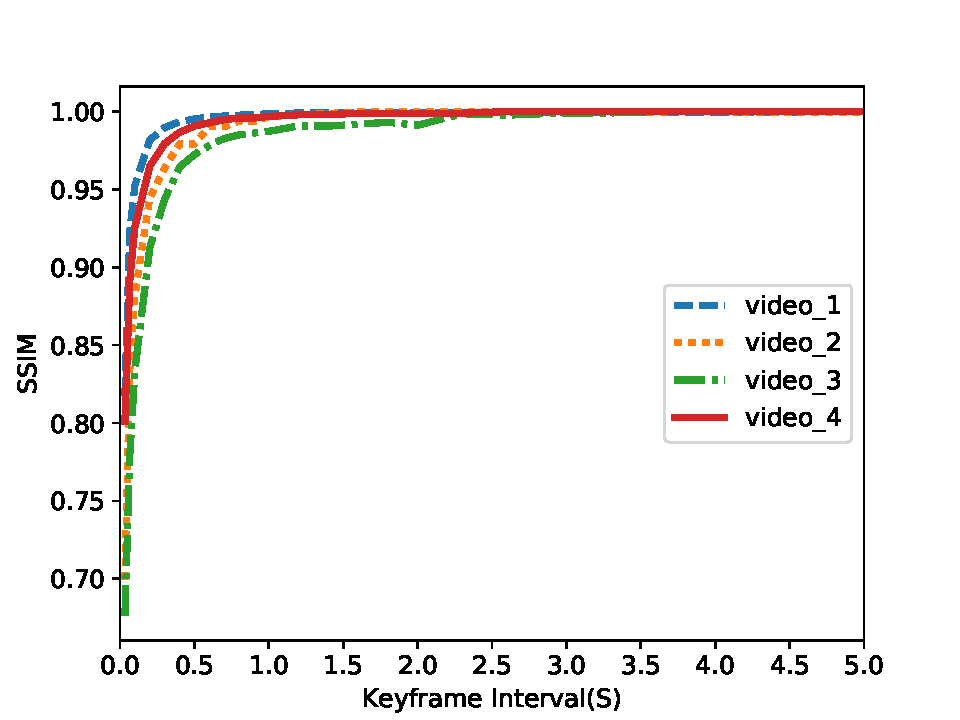
\includegraphics[width=0.7\textwidth]{ssim_gop}
  \caption{不同关键帧间隔时视频编码后的SSIM}
  \label{fig:ssim_gop}
\end{figure}

\section{智能丢帧策略}
为了衡量丢帧算法的性能优化效果,我们选择了两个算法作为对比,离线最优算法Oracle和默认算法OBS。Oracle,通过暴力搜索加剪枝可以达到离线最优,但时间复杂度在指数级别。我们从带宽数据集中任意选择其中一段,时长为30秒附近。利用上一小节的结论,关键帧间隔的选择范围为$[0.5,2]$秒,我们将关键帧间隔设置为1秒。为了研究算法优化丢帧的效果,在三组实验中我们将码率都固定在2850kbps,小于初始带宽值,但远大于衰落之后的带宽值。合理的码率选择使得这段数据既包含长时间的带宽抖动,也包括瞬时的带宽抖动。

\begin{figure}[tb]
  \centering%
  \begin{subfigure}{0.49\textwidth}
    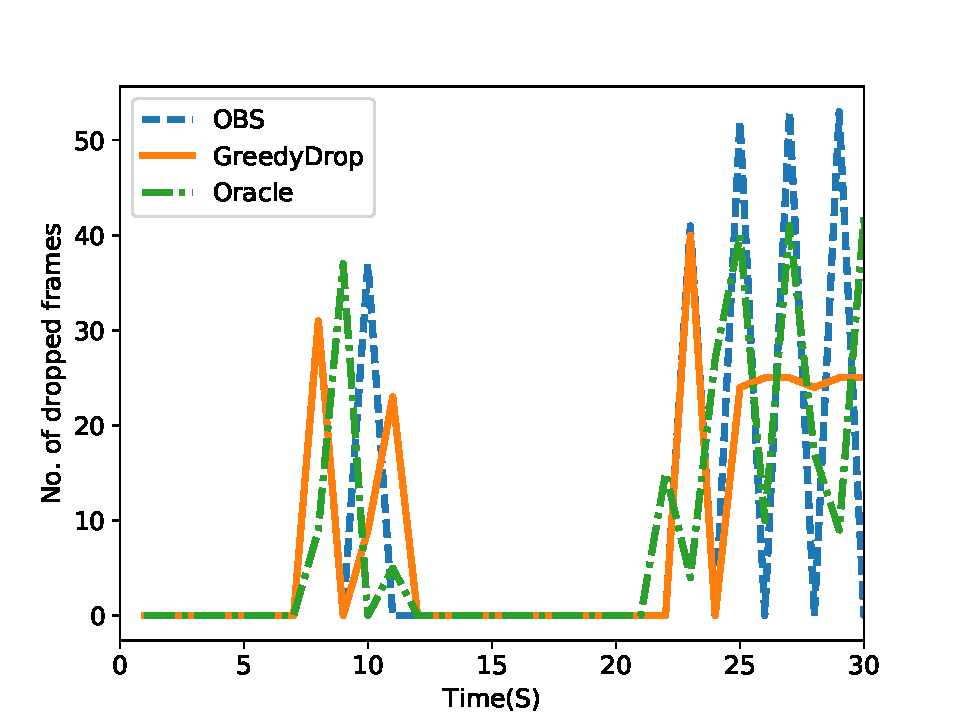
\includegraphics[width=\textwidth]{drop-buffer}
    \caption{实时丢帧数}
    \label{fig:drop-buffer}
  \end{subfigure}%
  \hfill
  \begin{subfigure}{0.49\textwidth}
    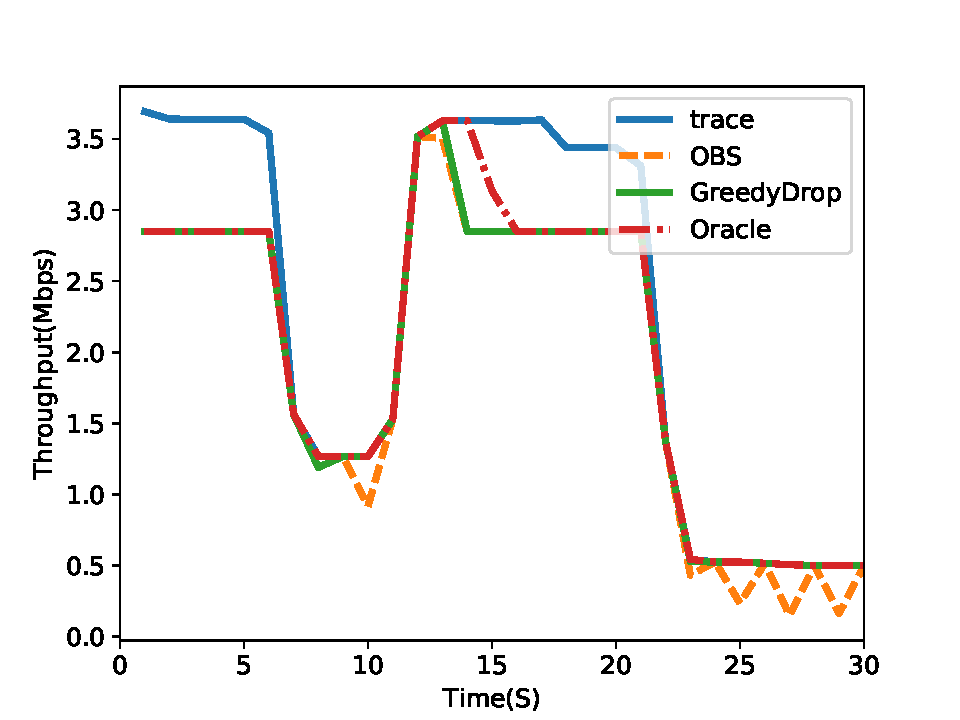
\includegraphics[width=\textwidth]{drop-bandwidth}
    \caption{实时的吞吐量}
    \label{fig:drop-bandwidth}
  \end{subfigure}
  \caption{不同丢帧策略性能比较}
  \label{fig:drop_comparison}
\end{figure}

丢帧的减少程度在表~\ref{tab_drop}中给出。上传失败时长定义为丢帧数对应的播放时长,计算公式为上传失败时长=丢帧数/帧率。

\begin{table}[tb]
\centering
\caption{与默认OBS算法相比丢帧的减少程度}
\label{tab_drop}
{\setlength{\tabcolsep}{2pt}
\begin{tabular}{|c|c|c|l|}
\hline
\textbf{算法} &\textbf{丢帧数} &\textbf{上传失败时长(秒)} & \textbf{与默认OBS算法相比丢帧对应的百分比}    \\ \hline
Oracle    &265  &8.83  &$80\%$           \\ \hline
GreedyDrop  &274 &9.13  &$85.6\%$              \\ \hline
OBS默认算法     &320  &10.67  &无 \\ \hline
\end{tabular}}
\end{table}

三种算法中,默认OBS算法丢帧数最多,上传失败时长最长,GreedyDrop智能丢帧算法减少了15\%的上传失败,改善丢帧的效果较为明显。而且GreedyDrop在线算法和离线最优Oracle算法之间的差距较小,约等于5\%左右。实时丢帧数和真实吞吐量的时序图展示在图~\ref{fig:drop_comparison}中。丢帧主要发生的时间段位于7到12秒和20到30秒期间。7到12秒时三种算法的表现基本相同,实时带宽紧跟控制数据一起变化;因为Oracle算法知道网络恢复的具体时间,相对于其他算法,会在视频队列中保存更多的有效帧,当网络状况恢复后,10到15秒期间时Oracle算法会将队列中的视频帧以burst的形式发送出去,相比于其他两个算法,避免了一部分丢帧。20到30秒期间,网络经历着长时间的带宽抖动,OBS算法的丢帧数呈现周期性的振荡变化,方差很大,而GreedyDrop算法基本每个时刻的丢帧都很稳定。因为GreedyDrop算法只丢弃视频队列中属于旧的GoP的帧,而OBS算法每次丢帧将队列中的帧全部丢弃,因为丢帧行为会呈现一定的周期性。对于GreedyDrop算法,每个GoP开头的帧被发送出去,剩余的帧都被丢弃,规律性的行为使得丢帧数和吞吐量都保持恒定。Oracle算法和OBS算法的性能类似,每个时刻的丢帧数有一定的波动,但是方差变化比较小。同时考虑时间复杂度和算法性能,GreedyDrop是个不错的选择。

\section{自适应码率算法}
我们选取了几个在视频点播方面性能很好的动态码率算法,作为对比算法,来和GVBR算法做比较。为了控制变量,保持对比算法的一致性,和GVBR算法一样,对比算法中我们依然用调和平均值来作为对带宽的预估。
\begin{itemize}
  \item OBS-VBR:简单直接的码率自适应算法,和OBS默认算法基本一致,使用OBS默认的丢帧策略,唯一的不同点在于动态码率,每个时刻都选择比估计带宽低的最高可用码率。
  \item MPC:用队列状态信息(帧数和帧的大小,以及帧的类型)和预测带宽值去计算接下来几个时隙的最优码率选择,但只应用第一个时隙的码率选择,对于之后的时隙重复上述过程。
  \item Robust-MPC:使用和MPC类似的方法,唯一的不同点,在于用过去几个时隙的最大预测误差去矫正未来几个时隙的带宽估计。
\end{itemize}
除了OBS-VBR算法之外,上述的几个对比算法均用GreedyDrop作为丢帧策略。Robust-MPC是视频点播领域最先进的码率自适应算法,MPC算法和Robust-MPC算法均是使用模型预测控制理论去选择未来时隙的码率。模型预测控制理论,简称MPC,主要的思想是预测未来几个时隙的带宽和系统状态,计算几个时隙的最优选择,但在应用时只用第一个时隙的选择,这个理论可以直接应用到直播场景中去,因此我们选择将Robust-MPC和MPC作为我们的直播动态码率对比算法。

\begin{figure}[tb]
  \centering%
  \begin{subfigure}{0.5\textwidth}
    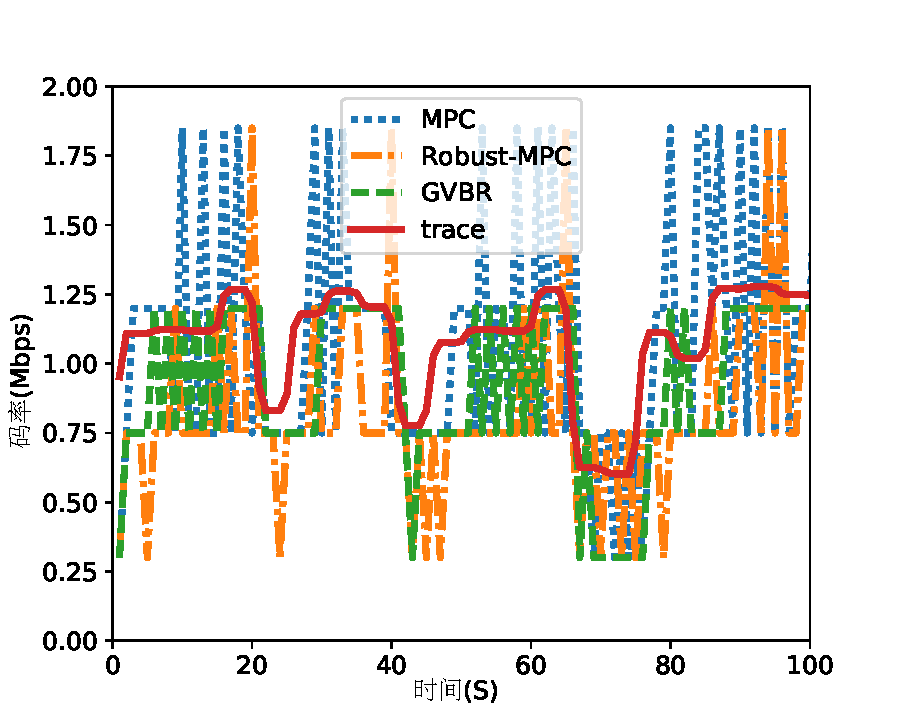
\includegraphics[width=\textwidth]{specific_fcc}
    \caption{FCC数据集的实时吞吐量}
    \label{fig:fcc}
  \end{subfigure}%
  \hfill
  \begin{subfigure}{0.5\textwidth}
    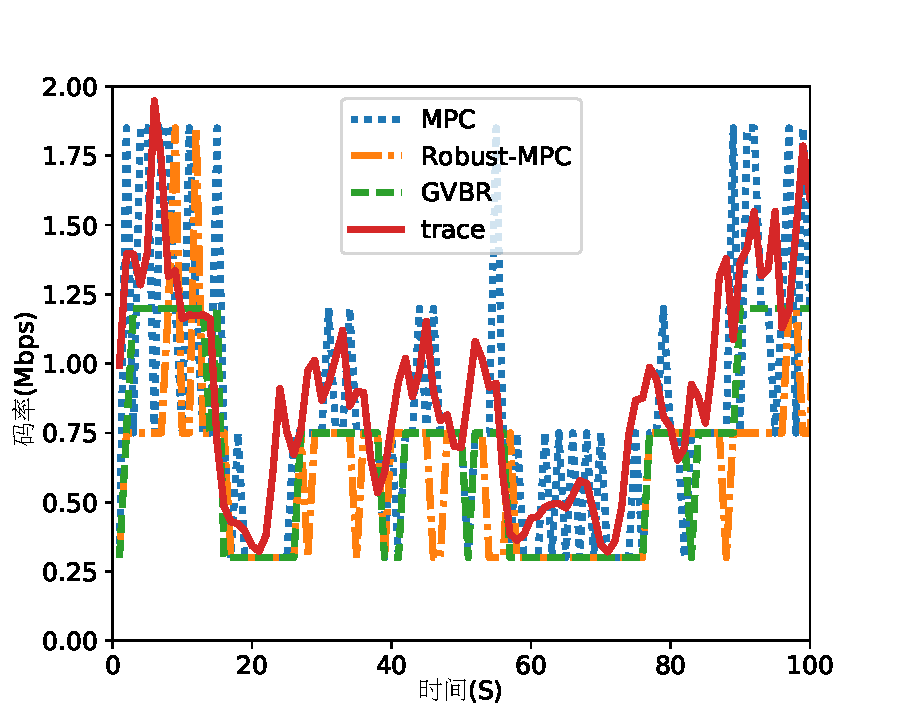
\includegraphics[width=\textwidth]{specific_hsdpa}
    \caption{HSDPA数据集的实时吞吐量}
    \label{fig:hsdpa}
  \end{subfigure}
  \caption{不同码率自适应算法吞吐量比较}
  \label{fig:specific}
\end{figure}

详细的对比算法结果展示在图~\ref{fig:specific}中。图~\ref{fig:fcc}和图~\ref{fig:hsdpa}分别展示了FCC数据集和HSDPA数据集下三种算法的性能。在这两幅图中,实线代表着真实世界的带宽数据记录。相比于Robust-MPC,MPC缺少对预测误差的矫正,容易更激进的选择更高的码率,反映到图中,MPC每个时刻的码率总是高于Robust-MPC的码率。除此之外,两个MPC算法的码率总是在真实带宽附近波动。两种数据集下,MPC和Robust-MPC的码率切换都比GVBR更频繁。这是因为GVBR的策略是选择比带宽低的最高码率,当带宽波动较小时,GVBR很有发生变化。但是MPC的策略是选择一个使用户体验质量最高的码率,当带宽稍微波动一点,MPC会更加倾向于选择一个更高或码率,增大优化目标中的第一项,码率相关的效益。而Robust-MPC虽然增加了对于预测误差的矫正,但依然是求几个时隙的最优选择,和MPC的行为较为类似。

\begin{figure}[tb]% use float package if you want it here
  \centering
  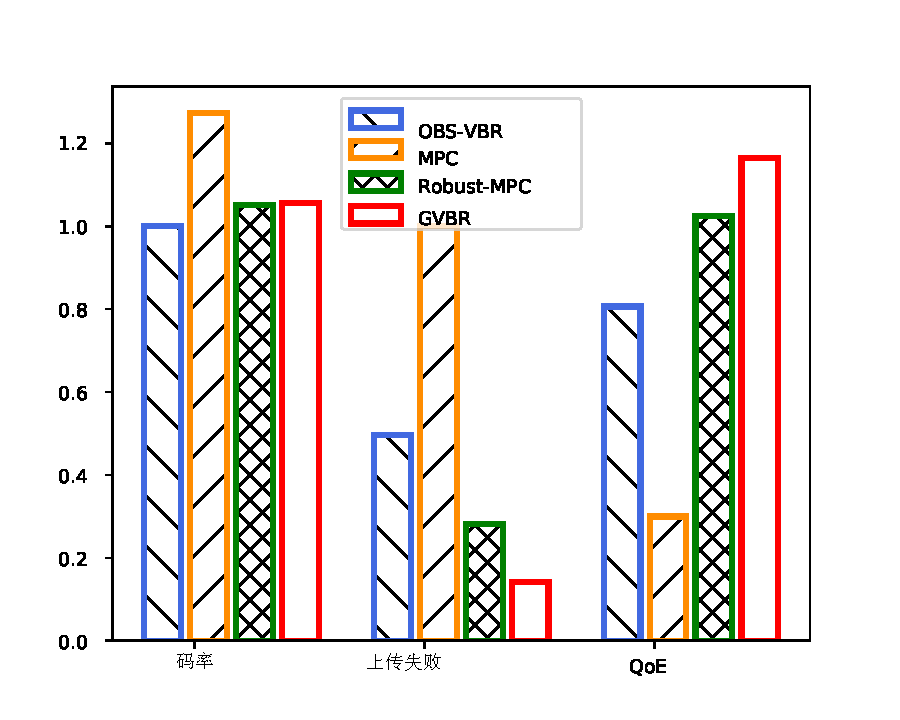
\includegraphics[width=0.7\textwidth]{massive_qoe}
  \caption{归一化平均码率,上传失败时长和用户体验质量}
  \label{fig:massive_qoe}
\end{figure}

大规模的仿真实验结果展示在图~\ref{fig:massive_qoe}中,我们结合两个数据集去评估GVBR算法的性能,分别是FCC数据集和HSDPA数据集。图中展示的三项指标,码率,上传失败时长和用户体验质量都是归一化之后的平均指标。四种算法中,MPC拥最高的码率效益,这是因为MPC的带宽估计算法很激进,会更倾向于选择较高的码率。其他三种算法有着基本相同的平均码率,其中GVBR和Robust-MPC两种算法的平均码率稍微高一点,高于OBS-VBR算法。虽然MPC达到了最高的码率水平,但也带来了最高的丢帧数,对应的平均上传失败的时间也最长。OBS-VBR算法使用的丢帧算法是默认的OBS丢帧策略,所以在剩余三种算法中上传失败的时长最高。Robust-MPC算法相对于MPC算法来说增加了对于预测误差的纠正,将上传失败时间减少到可以忍受的时长。因为考虑了队列中排队等待发送的视频帧的数据量,GVBR将平均上传失败的时长减少到很少的时间,相对于Robust-MPC减少了50\%左右。平均码率略微高于多个对比算法,而且平均上传失败时长很短,GVBR的用户体验质量在所有算法中达到了最高水平。剩余三种算法的用户体验质量排序分别是Robust-MPC,OBS-VBR和MPC。

\begin{figure}[tb]
  \centering%
  \begin{subfigure}{0.48\textwidth}
    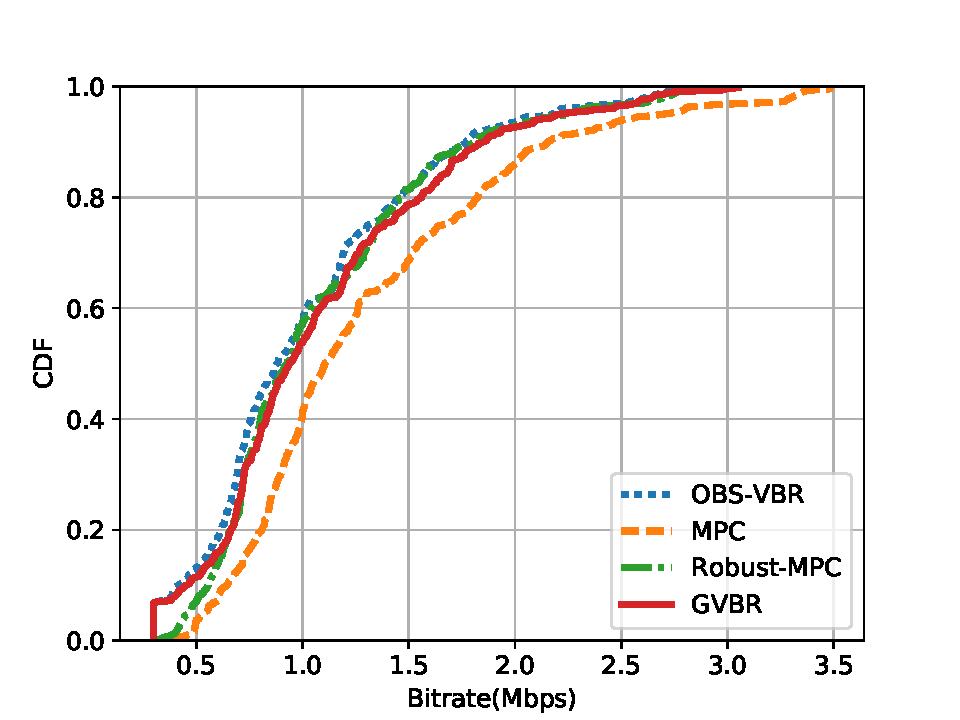
\includegraphics[width=\textwidth]{massive-bitrate-cdf}
    \caption{平均码率累计分布图}
    \label{fig:bitrate_cdf}
  \end{subfigure}%
  \hfill
  \begin{subfigure}{0.48\textwidth}
    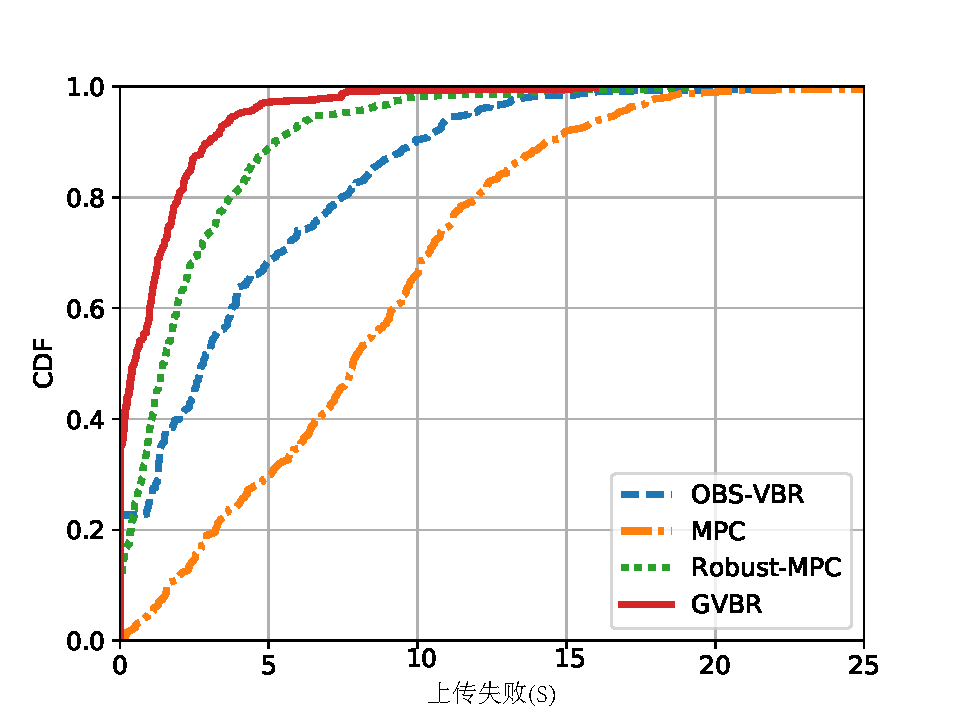
\includegraphics[width=\textwidth]{massive-drop-cdf}
    \caption{上传失败时长累计分布图}
    \label{fig:drop_cdf}
  \end{subfigure}
  \vfill
  \vspace{0.2in}
  \begin{subfigure}{0.48\textwidth}
    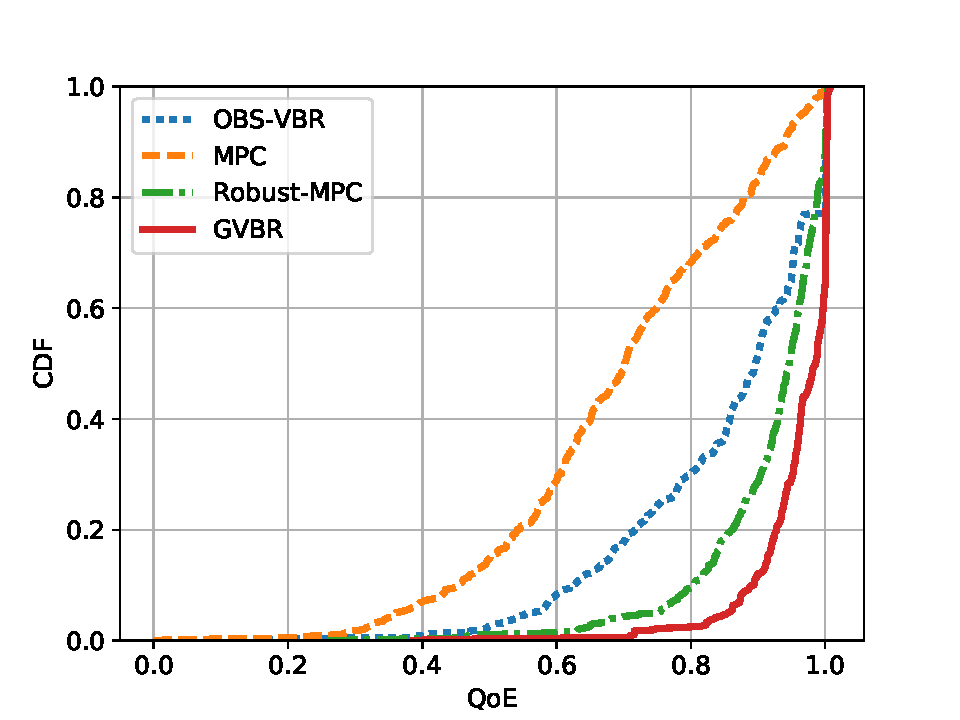
\includegraphics[width=\textwidth]{massive-qoe-cdf}
    \caption{归一化用户体验质量累计分布图}
    \label{fig:qoe_cdf}
  \end{subfigure}
  \caption{大规模实验结果图}
  \label{fig:massive_cdf}
\end{figure}

平均码率,平均上传失败时长和平均用户体验质量的累计分布图展示在图~\ref{fig:massive_cdf}中。在图~\ref{fig:bitrate_cdf}中,GVBR算法位于Robust-MPC和OBS算法的右边,码率值稍微高于这两者。
MPC位于其余三种算法的右边,码率值远远高于其他三种算法,和图~\ref{fig:massive_qoe}的结论一致。从图~\ref{fig:drop_cdf}中可以看出,对于GVBR算法,98\%的实验其上传失败时间都低于5秒,有大约40\%的的实验中未出现过上传失败。
而其余三种算法低于5秒上传失败时间的百分比分别是,Robust-MPC有90\%的实验上传失败时长低于5秒,OBS-VBR有70\%的实验,MPC只有30\%的实验。
图~\ref{fig:qoe_cdf}显示,GVBR算法只有2\%的实验中用户体验质量不是很好,其余的98\%的情况下归一化用户体验质量大约在$[0.8,1]$之间。剩余三种算法的归一化用户体验质量大于80\%的比例分别是,MPC为30\%,OBS-VBR为70\%,Robust-MPC为90\%。
总而言之,我们的GVBR算法在上传失败时长和用户体验质量两个指标上远远优于其他几个算法。

\begin{table}[tb]
\centering
\caption{码率自适应算法效果对比}
\label{tab:vbr}
{\setlength{\tabcolsep}{2pt}
\begin{tabular}{|c|c|c|l|}
\hline
\textbf{算法} &\textbf{平均码率(Mbps)} &\textbf{平均上传失败时长(秒)} & \textbf{平均用户体验质量}    \\ \hline
OBS    &1.0788  &26.1438  &-39107.835           \\ \hline
OBS-VBR  &1.0256 &3.9763  &-5862.833         \\ \hline
MPC     &1.3060  &8.0017  &-11877.126 \\ \hline
Robust-MPC &1.0781 &2.2553 &-3281.921 \\ \hline
GVBR &1.0821 &1.1414 &-1605.033 \\ \hline
\end{tabular}}
\end{table}

由于固定码率的OBS默认算法和四种自适应码率算法的性能差别过大,上述性能比较图中未出现默认OBS算法的对比。我们将默认OBS算法和几种动态码率算法的对比结果整理在表~\ref{tab:vbr}中。相比于最原始的固定码率OBS算法,GVBR算法减少了95.6\%的丢帧。
原始的OBS算法平均上传失败时长是26秒,而我们的GVBR算法只有1秒的平均失败时长。除了MPC算法之外,GVBR算法拥有最高的平均码率,略微高于其他三种算法。总的来说,我们的GVBR算法实现了更高的码率,与此同时显著减少了上传失败的发生。另外,
表中可以得到的一个结论是,运用自适应码率算法之后可以大幅度减少上传失败现象的发生。

\section{本章小结}
本章对于提出的优化方案进行了系统的性能评估,主要包括不同层面的方案,GoP层面的减少关键帧间隔以及码率自适应算法,GoP内部的智能丢帧策略。

首先,本章针对关键帧间隔大小对视频质量的影响进行了评估,发现了当关键帧间隔减少到一定值之后,视频质量呈现急剧下降,严重损害用户的观看体验。
为了避免这种现象,关键帧间隔在选取时应严格遵循最小取值的约束,减少丢帧现象发生的同时保证视频质量。

其次,对于棘手的丢帧策略选择,我们对比了离线最优算法和GreedyDrop算法的优劣。相比于默认的OBS丢帧策略,GreedyDrop和离线最优算法的性能明显优于前面两者。
但是离线最优算法的时间复杂度为指数级,对于移动设备的计算性能要求太高,而且离线最优算法需要已知全程的带宽状况,这在实际中是不可行的。综合时间复杂度和对于减少丢帧的性能改善,GreedyDrop算法是较优的选择。

最后,对于我们最后提出的一整套的解决方案GVBR,进行了充分的性能评估。不仅与视频点播领域较为先进的码率自适应算法MPC对比,而且和最原始的默认OBS算法进行了对比。
实验结果显示,除了在平均码率的指标上略逊色于MPC算法,在平均上传失败时长和用户体验质量方面远远优于其他几种算法。

\chapter{总结和展望}
\section{论文工作总结}
随着近几年移动设备的普及和通信技术的发展,移动网络直播的用户规模呈现爆炸式增长,研究如何优化移动直播的用户体验质量越来越重要。移动直播中主播端因为占据着源端的至关重要地位,主播端在上传过程中发生的任何延迟和失败都会对所有的观看用户产生影响。但是移动主播一般都处在无线网络环境下,网络状况较为较为复杂。无线网络环境下移动主播经常需要和其他人一起竞争带宽,同时由于直播过程中主播的移动,周围环境的信号干扰等各种原因,带宽抖动的情况经常会发生。而且移动直播要求用户和主播间有高互动性,端到端的时延最多为几秒,这些因素都为优化用户体验带来了很大的挑战。本文对移动网络环境下主播端存在的性能问题进行研究,提出了一整套的协同解决方案,旨在通过优化主播端的传输性能去优化用户端的体验质量。

首先,本文通过对搭建的demo直播系统的性能测量,发现了移动直播过程中由于网络带宽抖动会导致两种质量问题,分别是短时的带宽抖动带来的应用层丢帧放大效应,以及长时间的带宽抖动带来的上传视频质量降低等问题。为了验证商业直播平台是否也存在类似的问题,我们选取了2个推流端,2个视频服务器组合起来,测量无线网络环境下商业平台的性能。通过实际的测量发现,商业平台也存在以上的两种问题,并不能很好的解决无线网络带来的质量问题。

为了解决上述问题,我们从三个方向进行了探索,涉及了GoP内部优化和GoP整体优化。我们提出的GVBR算法,是一整套提高主播端用户体验质量的协同解决方案,它修改了关键帧间隔的取值,改进了默认的丢帧策略,并且设计了一个有效的码率自适应算法。关键帧间隔的取值综合考虑了视频质量和丢帧现象等两个方面的影响,最后权衡两者给出了关键帧间隔的参考范围。修改后的丢帧策略GreedyDrop考虑了两个或多个GoP同时存在于视频队列中的情况,针对这种情况,GreedyDrop只丢弃旧的GoP的视频帧,保留较新的GoP相关的帧。GreedyDrop算法与离线最优算法Oracle之间的差距很小,只有5\%的差距,而且同时GreedyDrop时间复杂度也很小,为线性时间复杂度。GVBR则根据估计出的带宽和视频队列数据量的差值去选择码率,考虑到视频队列里的剩余数据量可以更精确的计算真实可用的带宽。实验结果表明GVBR相比于最先进的码率自适应算法减少了50\%的丢帧。对比最原始的默认OBS算法,我们提出的一整套协同解决方案,GVBR,将原始的上传失败时长从26秒减少到1秒,改进了95.6\%,同时大幅度改善了用户的体验质量。

\section{未来工作展望}
本文对个人交互直播主播端的用户体验优化研究仍存在不少欠缺的地方,后续的工作可以从下面两个可能的方向来进一步开展:

\textbf{使用新的带宽预测算法提升带宽预测的准确率}。因为本文主要研究的重点是优化主播端的传输性能,所以只是使用了一个现有的带宽预测方案。如果能够进一步提高带宽预测的准确度,相关算法的性能都会更上一个台阶。因此研究一个更加精确的带宽预测方案很有必要,这也是我们下一步工作的重点。

\textbf{将GVBR算法在实际系统中实现}。GVBR算法在设计时就考虑了实际部署的问题,算法的时间复杂度并不高,在实际部署中不会给移动设备带来很大的性能开销。 但实际系统运行的情况远比理论的情况要复杂得多,所以GVBR算法可能在未来应该更结合实际情况,去做一些相应的修改。


%%% 其它部分
\backmatter

%% 本科生要这几个索引,研究生不要。选择性留下。
% 插图索引
\listoffigures
% 表格索引
\listoftables
% 公式索引
\listofequations


%% 参考文献
% 注意:至少需要引用一篇参考文献,否则下面两行可能引起编译错误。
% 如果不需要参考文献,请将下面两行删除或注释掉。
% 数字式引用
\bibliographystyle{thuthesis-numeric}
% 作者-年份式引用
% \bibliographystyle{thuthesis-author-year}
\bibliography{ref/refs}


%% 致谢
% 如果使用声明扫描页,将可选参数指定为扫描后的 PDF 文件名,例如:
% \begin{acknowledgement}[scan-statement.pdf]
\begin{acknowledgement}
  衷心感谢导师 xxx 教授和物理系 xxx 副教授对本人的精心指导。他们的言传身教将使
  我终生受益。

  在美国麻省理工学院化学系进行九个月的合作研究期间,承蒙 xxx 教授热心指导与帮助,不
  胜感激。感谢 xx 实验室主任 xx 教授,以及实验室全体老师和同学们的热情帮助和支
  持!本课题承蒙国家自然科学基金资助,特此致谢。

  感谢 \LaTeX 和 \thuthesis\cite{thuthesis},帮我节省了不少时间。
\end{acknowledgement}


%% 附录
\begin{appendix}
\chapter{外文资料原文}
\label{cha:engorg}

\title{The title of the English paper}

\textbf{Abstract:} As one of the most widely used techniques in operations
research, \emph{ mathematical programming} is defined as a means of maximizing a
quantity known as \emph{bjective function}, subject to a set of constraints
represented by equations and inequalities. Some known subtopics of mathematical
programming are linear programming, nonlinear programming, multiobjective
programming, goal programming, dynamic programming, and multilevel
programming$^{[1]}$.

It is impossible to cover in a single chapter every concept of mathematical
programming. This chapter introduces only the basic concepts and techniques of
mathematical programming such that readers gain an understanding of them
throughout the book$^{[2,3]}$.


\section{Single-Objective Programming}
The general form of single-objective programming (SOP) is written
as follows,
\begin{equation}\tag*{(123)} % 如果附录中的公式不想让它出现在公式索引中,那就请
                             % 用 \tag*{xxxx}
\left\{\begin{array}{l}
\max \,\,f(x)\\[0.1 cm]
\mbox{subject to:} \\ [0.1 cm]
\qquad g_j(x)\le 0,\quad j=1,2,\cdots,p
\end{array}\right.
\end{equation}
which maximizes a real-valued function $f$ of
$x=(x_1,x_2,\cdots,x_n)$ subject to a set of constraints.

\newtheorem{mpdef}{Definition}[chapter]
\begin{mpdef}
In SOP, we call $x$ a decision vector, and
$x_1,x_2,\cdots,x_n$ decision variables. The function
$f$ is called the objective function. The set
\begin{equation}\tag*{(456)} % 这里同理,其它不再一一指定。
S=\left\{x\in\Re^n\bigm|g_j(x)\le 0,\,j=1,2,\cdots,p\right\}
\end{equation}
is called the feasible set. An element $x$ in $S$ is called a
feasible solution.
\end{mpdef}

\newtheorem{mpdefop}[mpdef]{Definition}
\begin{mpdefop}
A feasible solution $x^*$ is called the optimal
solution of SOP if and only if
\begin{equation}
f(x^*)\ge f(x)
\end{equation}
for any feasible solution $x$.
\end{mpdefop}

One of the outstanding contributions to mathematical programming was known as
the Kuhn-Tucker conditions\ref{eq:ktc}. In order to introduce them, let us give
some definitions. An inequality constraint $g_j(x)\le 0$ is said to be active at
a point $x^*$ if $g_j(x^*)=0$. A point $x^*$ satisfying $g_j(x^*)\le 0$ is said
to be regular if the gradient vectors $\nabla g_j(x)$ of all active constraints
are linearly independent.

Let $x^*$ be a regular point of the constraints of SOP and assume that all the
functions $f(x)$ and $g_j(x),j=1,2,\cdots,p$ are differentiable. If $x^*$ is a
local optimal solution, then there exist Lagrange multipliers
$\lambda_j,j=1,2,\cdots,p$ such that the following Kuhn-Tucker conditions hold,
\begin{equation}
\label{eq:ktc}
\left\{\begin{array}{l}
    \nabla f(x^*)-\sum\limits_{j=1}^p\lambda_j\nabla g_j(x^*)=0\\[0.3cm]
    \lambda_jg_j(x^*)=0,\quad j=1,2,\cdots,p\\[0.2cm]
    \lambda_j\ge 0,\quad j=1,2,\cdots,p.
\end{array}\right.
\end{equation}
If all the functions $f(x)$ and $g_j(x),j=1,2,\cdots,p$ are convex and
differentiable, and the point $x^*$ satisfies the Kuhn-Tucker conditions
(\ref{eq:ktc}), then it has been proved that the point $x^*$ is a global optimal
solution of SOP.

\subsection{Linear Programming}
\label{sec:lp}

If the functions $f(x),g_j(x),j=1,2,\cdots,p$ are all linear, then SOP is called
a {\em linear programming}.

The feasible set of linear is always convex. A point $x$ is called an extreme
point of convex set $S$ if $x\in S$ and $x$ cannot be expressed as a convex
combination of two points in $S$. It has been shown that the optimal solution to
linear programming corresponds to an extreme point of its feasible set provided
that the feasible set $S$ is bounded. This fact is the basis of the {\em simplex
  algorithm} which was developed by Dantzig as a very efficient method for
solving linear programming.
\begin{table}[ht]
\centering
  \centering
  \caption*{Table~1\hskip1em This is an example for manually numbered table, which
    would not appear in the list of tables}
  \label{tab:badtabular2}
  \begin{tabular}[c]{|m{1.5cm}|c|c|c|c|c|c|}\hline
    \multicolumn{2}{|c|}{Network Topology} & \# of nodes &
    \multicolumn{3}{c|}{\# of clients} & Server \\\hline
    GT-ITM & Waxman Transit-Stub & 600 &
    \multirow{2}{2em}{2\%}&
    \multirow{2}{2em}{10\%}&
    \multirow{2}{2em}{50\%}&
    \multirow{2}{1.2in}{Max. Connectivity}\\\cline{1-3}
    \multicolumn{2}{|c|}{Inet-2.1} & 6000 & & & &\\\hline
    \multirow{2}{1.5cm}{Xue} & Rui  & Ni &\multicolumn{4}{c|}{\multirow{2}*{\thuthesis}}\\\cline{2-3}
    & \multicolumn{2}{c|}{ABCDEF} &\multicolumn{4}{c|}{} \\\hline
\end{tabular}
\end{table}

Roughly speaking, the simplex algorithm examines only the extreme points of the
feasible set, rather than all feasible points. At first, the simplex algorithm
selects an extreme point as the initial point. The successive extreme point is
selected so as to improve the objective function value. The procedure is
repeated until no improvement in objective function value can be made. The last
extreme point is the optimal solution.

\subsection{Nonlinear Programming}

If at least one of the functions $f(x),g_j(x),j=1,2,\cdots,p$ is nonlinear, then
SOP is called a {\em nonlinear programming}.

A large number of classical optimization methods have been developed to treat
special-structural nonlinear programming based on the mathematical theory
concerned with analyzing the structure of problems.
\begin{figure}[h]
  \centering
  
\includegraphics{thu-lib-logo}
  \caption*{Figure~1\quad This is an example for manually numbered figure,
    which would not appear in the list of figures}
  \label{tab:badfigure2}
\end{figure}

Now we consider a nonlinear programming which is confronted solely with
maximizing a real-valued function with domain $\Re^n$.  Whether derivatives are
available or not, the usual strategy is first to select a point in $\Re^n$ which
is thought to be the most likely place where the maximum exists. If there is no
information available on which to base such a selection, a point is chosen at
random. From this first point an attempt is made to construct a sequence of
points, each of which yields an improved objective function value over its
predecessor. The next point to be added to the sequence is chosen by analyzing
the behavior of the function at the previous points. This construction continues
until some termination criterion is met. Methods based upon this strategy are
called {\em ascent methods}, which can be classified as {\em direct methods},
{\em gradient methods}, and {\em Hessian methods} according to the information
about the behavior of objective function $f$. Direct methods require only that
the function can be evaluated at each point. Gradient methods require the
evaluation of first derivatives of $f$. Hessian methods require the evaluation
of second derivatives. In fact, there is no superior method for all
problems. The efficiency of a method is very much dependent upon the objective
function.

\subsection{Integer Programming}

{\em Integer programming} is a special mathematical programming in which all of
the variables are assumed to be only integer values. When there are not only
integer variables but also conventional continuous variables, we call it {\em
  mixed integer programming}. If all the variables are assumed either 0 or 1,
then the problem is termed a {\em zero-one programming}. Although integer
programming can be solved by an {\em exhaustive enumeration} theoretically, it
is impractical to solve realistically sized integer programming problems. The
most successful algorithm so far found to solve integer programming is called
the {\em branch-and-bound enumeration} developed by Balas (1965) and Dakin
(1965). The other technique to integer programming is the {\em cutting plane
  method} developed by Gomory (1959).

\hfill\textit{Uncertain Programming\/}\quad(\textsl{BaoDing Liu, 2006.2})

\section*{References}
\noindent{\itshape NOTE: These references are only for demonstration. They are
  not real citations in the original text.}

\begin{translationbib}
\item Donald E. Knuth. The \TeX book. Addison-Wesley, 1984. ISBN: 0-201-13448-9
\item Paul W. Abrahams, Karl Berry and Kathryn A. Hargreaves. \TeX\ for the
  Impatient. Addison-Wesley, 1990. ISBN: 0-201-51375-7
\item David Salomon. The advanced \TeX book.  New York : Springer, 1995. ISBN:0-387-94556-3
\end{translationbib}

\chapter{外文资料的调研阅读报告或书面翻译}

\title{英文资料的中文标题}

{\heiti 摘要:} 本章为外文资料翻译内容。如果有摘要可以直接写上来,这部分好像没有
明确的规定。

\section{单目标规划}
北冥有鱼,其名为鲲。鲲之大,不知其几千里也。化而为鸟,其名为鹏。鹏之背,不知其几
千里也。怒而飞,其翼若垂天之云。是鸟也,海运则将徙于南冥。南冥者,天池也。
\begin{equation}\tag*{(123)}
 p(y|\mathbf{x}) = \frac{p(\mathbf{x},y)}{p(\mathbf{x})}=
\frac{p(\mathbf{x}|y)p(y)}{p(\mathbf{x})}
\end{equation}

吾生也有涯,而知也无涯。以有涯随无涯,殆已!已而为知者,殆而已矣!为善无近名,为
恶无近刑,缘督以为经,可以保身,可以全生,可以养亲,可以尽年。

\subsection{线性规划}
庖丁为文惠君解牛,手之所触,肩之所倚,足之所履,膝之所倚,砉然响然,奏刀騞然,莫
不中音,合于桑林之舞,乃中经首之会。
\begin{table}[ht]
\centering
  \centering
  \caption*{表~1\hskip1em 这是手动编号但不出现在索引中的一个表格例子}
  \label{tab:badtabular3}
  \begin{tabular}[c]{|m{1.5cm}|c|c|c|c|c|c|}\hline
    \multicolumn{2}{|c|}{Network Topology} & \# of nodes &
    \multicolumn{3}{c|}{\# of clients} & Server \\\hline
    GT-ITM & Waxman Transit-Stub & 600 &
    \multirow{2}{2em}{2\%}&
    \multirow{2}{2em}{10\%}&
    \multirow{2}{2em}{50\%}&
    \multirow{2}{1.2in}{Max. Connectivity}\\\cline{1-3}
    \multicolumn{2}{|c|}{Inet-2.1} & 6000 & & & &\\\hline
    \multirow{2}{1.5cm}{Xue} & Rui  & Ni &\multicolumn{4}{c|}{\multirow{2}*{\thuthesis}}\\\cline{2-3}
    & \multicolumn{2}{c|}{ABCDEF} &\multicolumn{4}{c|}{} \\\hline
\end{tabular}
\end{table}

文惠君曰:“嘻,善哉!技盖至此乎?”庖丁释刀对曰:“臣之所好者道也,进乎技矣。始臣之
解牛之时,所见无非全牛者;三年之后,未尝见全牛也;方今之时,臣以神遇而不以目视,
官知止而神欲行。依乎天理,批大郤,导大窾,因其固然。技经肯綮之未尝,而况大坬乎!
良庖岁更刀,割也;族庖月更刀,折也;今臣之刀十九年矣,所解数千牛矣,而刀刃若新发
于硎。彼节者有间而刀刃者无厚,以无厚入有间,恢恢乎其于游刃必有余地矣。是以十九年
而刀刃若新发于硎。虽然,每至于族,吾见其难为,怵然为戒,视为止,行为迟,动刀甚微,
謋然已解,如土委地。提刀而立,为之而四顾,为之踌躇满志,善刀而藏之。”

文惠君曰:“善哉!吾闻庖丁之言,得养生焉。”


\subsection{非线性规划}
孔子与柳下季为友,柳下季之弟名曰盗跖。盗跖从卒九千人,横行天下,侵暴诸侯。穴室枢
户,驱人牛马,取人妇女。贪得忘亲,不顾父母兄弟,不祭先祖。所过之邑,大国守城,小
国入保,万民苦之。孔子谓柳下季曰:“夫为人父者,必能诏其子;为人兄者,必能教其弟。
若父不能诏其子,兄不能教其弟,则无贵父子兄弟之亲矣。今先生,世之才士也,弟为盗
跖,为天下害,而弗能教也,丘窃为先生羞之。丘请为先生往说之。”
\begin{figure}[h]
  \centering
  
\includegraphics{thu-whole-logo}
  \caption*{图~1\hskip1em 这是手动编号但不出现索引中的图片的例子}
  \label{tab:badfigure3}
\end{figure}

柳下季曰:“先生言为人父者必能诏其子,为人兄者必能教其弟,若子不听父之诏,弟不受
兄之教,虽今先生之辩,将奈之何哉?且跖之为人也,心如涌泉,意如飘风,强足以距敌,
辩足以饰非。顺其心则喜,逆其心则怒,易辱人以言。先生必无往。”

孔子不听,颜回为驭,子贡为右,往见盗跖。

\subsection{整数规划}
盗跖乃方休卒徒大山之阳,脍人肝而餔之。孔子下车而前,见谒者曰:“鲁人孔丘,闻将军
高义,敬再拜谒者。”谒者入通。盗跖闻之大怒,目如明星,发上指冠,曰:“此夫鲁国之
巧伪人孔丘非邪?为我告之:尔作言造语,妄称文、武,冠枝木之冠,带死牛之胁,多辞缪
说,不耕而食,不织而衣,摇唇鼓舌,擅生是非,以迷天下之主,使天下学士不反其本,妄
作孝弟,而侥幸于封侯富贵者也。子之罪大极重,疾走归!不然,我将以子肝益昼餔之膳。”


\chapter{其它附录}
前面两个附录主要是给本科生做例子。其它附录的内容可以放到这里,当然如果你愿意,可
以把这部分也放到独立的文件中,然后将其 \cs{input} 到主文件中。

\end{appendix}

%% 个人简历
\begin{resume}

  \resumeitem{个人简历}

  1992 年 8 月 16 日出生于 安徽 省 淮北市 。

  2011 年 9 月考入 北京邮电大学 大学 信息与通信工程学院 系 通信工程 专业,2015 年 7 月本科毕业并获得 工学 学士学位。

  2015 年 9 月免试进入 清华 大学 计算机科学与技术 系攻读 硕士 学位至今。

  \researchitem{发表的学术论文} % 发表的和录用的合在一起

  % 1. 已经刊载的学术论文(本人是第一作者,或者导师为第一作者本人是第二作者)
  \begin{publications}
    \item Yang Y, Ren T L, Zhang L T, et al. Miniature microphone with silicon-
      based ferroelectric thin films. Integrated Ferroelectrics, 2003,
      52:229-235. (SCI 收录, 检索号:758FZ.)
    \item 杨轶, 张宁欣, 任天令, 等. 硅基铁电微声学器件中薄膜残余应力的研究. 中国机
      械工程, 2005, 16(14):1289-1291. (EI 收录, 检索号:0534931 2907.)
    \item 杨轶, 张宁欣, 任天令, 等. 集成铁电器件中的关键工艺研究. 仪器仪表学报,
      2003, 24(S4):192-193. (EI 源刊.)
  \end{publications}

  % 2. 尚未刊载,但已经接到正式录用函的学术论文(本人为第一作者,或者
  %    导师为第一作者本人是第二作者)。
  \begin{publications}[before=\publicationskip,after=\publicationskip]
    \item Yang Y, Ren T L, Zhu Y P, et al. PMUTs for handwriting recognition. In
      press. (已被 Integrated Ferroelectrics 录用. SCI 源刊.)
  \end{publications}

  % 3. 其他学术论文。可列出除上述两种情况以外的其他学术论文,但必须是
  %    已经刊载或者收到正式录用函的论文。
  \begin{publications}
    \item Cui Y, Song J, Ren K, et al. Software defined cooperative offloading for mobile cloudlets[J]. IEEE/ACM Transactions on Networking, 2017, 25(3): 1746-1760. (SCI 收录, 检索号
      :896KM)
    \item Cui Y, Song J, Li M, et al. SDN-based big data caching in ISP networks[J]. IEEE Transactions on Big Data, 2017. (EI 收录, 检索号:06129773469)
  \end{publications}

  \researchitem{研究成果} % 有就写,没有就删除
  \begin{achievements}
    \item 崔勇, 宋健, 任青妹. 智能终端能耗优化的自适应流媒体分发方法: 中国, CN105245919B. (中国专利公布号.)
  \end{achievements}

\end{resume}


%% 本科生进行格式审查是需要下面这个表格,答辩可能不需要。选择性留下。
% 综合论文训练记录表
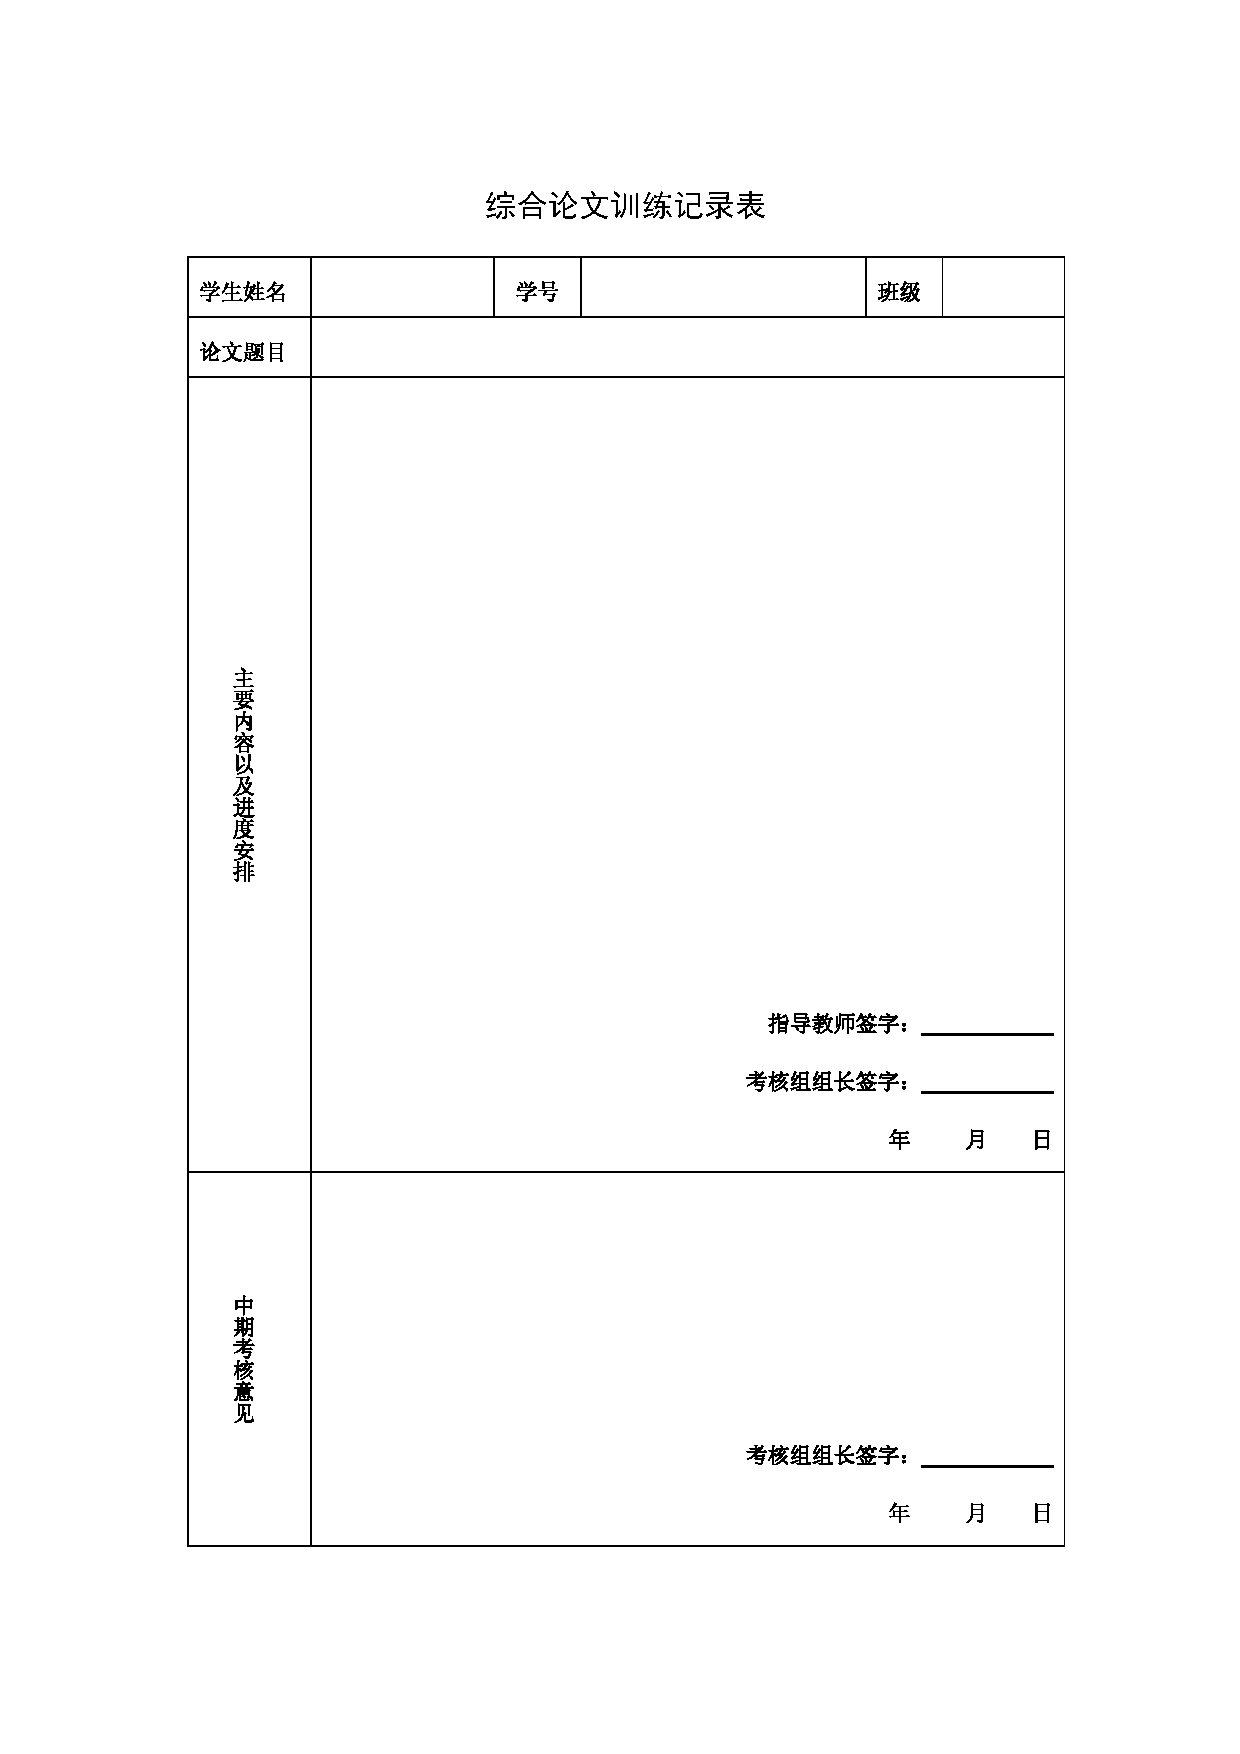
\includepdf[pages=-]{scan-record.pdf}
\end{document}
